\documentclass[
    fontsize=12pt,              % default font size 12pt
    paper=a4,                   % DIN A4 page format
    numbers=noenddot,           % remove dots behind chapter numbers (e.g. 1.5 not 1.5.)
    listof=totoc,               % add list of figures, tables, etc. to ToC
    listof=entryprefix,         % add entry name to figures, tables, etc.
    listof=nochaptergap,        % no chapter gap for figures, tables, etc.
    bibliography=totoc,         % add bibliography to ToC but without a chapter number
    parskip=half                % half line spacing between paragraphs
]{article}

% ##################################################
% ENCODING
% ##################################################
\usepackage{cmap}               % PDF character encoding
\usepackage[T1]{fontenc}        % 8-bit font encoding
\usepackage[utf8]{inputenc}     % UTF-8 input encoding

% ##################################################
% LANGUAGE
% ##################################################
\usepackage[ngerman]{babel} % Uncomment this if you write in German
\usepackage{csquotes}         % Package for better quotations
\hyphenation{}                % Here you can define custom hyphenations
\usepackage{blindtext}        % This package can usually be deleted as this is only used to display some blindtext

% ##################################################
% DOCUMENT VARIABLES
% ##################################################
% Personal data
\newcommand{\docAuthor}{Oliver Kusch}
\newcommand{\docMatriculationNumber}{268513}
\newcommand{\docStudyProgram}{Medieninformatik Master}
\newcommand{\docStudyFaculty}{Digitale Medien}
\newcommand{\docStudyDegree}{Master}
\newcommand{\docStreetName}{Erbsenlachen 6}
\newcommand{\docPostalCode}{78050}
\newcommand{\docCity}{Villingen-Schwenningen}
\newcommand{\docEmail}{oliver.kusch@hs-furtwangen.de}

% Document data
\newcommand{\docTitle}{Entwicklung einer Augmented Reality App zur Visualisierung historischer Gebäude der Stadt Villingen} % This is the main title of this document (thesis)
\newcommand{\docSubTitle}{}            % leave empty to remove
\newcommand{\docType}{Thesis}                            % Usually this will be 'Thesis"
\newcommand{\docSupervisor}{Prof. Dr. Uwe Hahne}             % Your supervisor
\newcommand{\docCoSupervisor}{Prof. Dr. Thomas Schneider}        % Your co-supervisor
\newcommand{\docDeadline}{31.08.2022}                      % This is the date when you submit the document

% ##################################################
% BIBLIOGRAPHY 
% ##################################################
\usepackage[backend=bibtex]{biblatex}
\addbibresource{literatur/library.bib}

\usepackage[acronym, toc, nogroupskip, nopostdot, nonumberlist]{glossaries}
\makeglossaries
\newacronym{ar}{AR}{Augmented Reality}

\newacronym{slam}{SLAM}{Simultaneous Localization and Mapping}



% ##################################################
% PDF SETTINGS
% ##################################################
\usepackage[
    colorlinks=true,
    linkcolor=black,
    citecolor=black,
    filecolor=black,
    urlcolor=black,
    bookmarks=true,
    bookmarksopen=true,
    bookmarksopenlevel=3,
    bookmarksnumbered,
    plainpages=false,
    pdfpagelabels=true,
    hyperfootnotes,
    pdftitle ={\docTitle},
    pdfauthor={\docAuthor},
    pdfcreator={\docAuthor}
]{hyperref}

% ##################################################
% FONTS AND SPACING
% ##################################################

\renewcommand{\baselinestretch}{1.5} % default 1.5 spacing
\raggedbottom                        % don't stretch spacing to fit page length
\usepackage{lmodern}                 % Allow font sizes at arbitrary sizes

% ##################################################
% PAGE FORMATTING
% ##################################################
% Page layout, see http://mirrors.ctan.org/macros/latex/contrib/geometry/geometry.pdf #3 Page geometry
\usepackage[
    bindingoffset=1.5cm, % Specify an offset if you plan to bind the document
    inner=2.5cm,         % Left Spacing
    outer=2.5cm,         % Right spacing
    top=3cm,             % Top spacing
    bottom=2cm,          % Bottom spacing
    twoside              % Delete this if you don't want to use double-sided pages
]{geometry}

% Page header
\usepackage[
    headsepline,                        % seperator line beneath page header on normal pages
    plainheadsepline                    % seperator line beneath page header on pages like ToC
]{scrlayer-scrpage}
\clearpairofpagestyles                  % clear default settings
\addtokomafont{pagehead}{\normalfont}   % use normal font for page header
\ohead*{\thepage}                       % page number
\ihead*{\leftmark}                      % chapter name
\setlength{\headheight}{18pt}           % set headheight to 18pt
\addtolength{\skip\footins}{0.5cm}      % spacing at the end of page (footnotes)
\usepackage[bottom]{footmisc}           % Always place footer at end of page

\usepackage{multicol}                   % Format text in multiple columns
\usepackage{emptypage}                  % Support for empty pages via \cleardoublepage
\usepackage{lscape}                     % Support for landscape pages

% ##################################################
% IMAGES AND FIGURES
% ##################################################
\usepackage{graphicx}                   % support for including images
\graphicspath{{img/}}                   % default path

% simple numbering without chapter
\renewcommand{\thefigure}{\arabic{figure}}

% ##################################################
% TikZ | Support for drawing diagrams
% ##################################################
\usepackage{tikz}
\usepackage{float}
\usetikzlibrary{shapes.geometric, arrows, positioning, decorations.pathreplacing, calc}
\tikzstyle{box} = [rectangle, minimum width=3cm, minimum height=1cm, text centered, draw=black, fill=orange!30]
\tikzstyle{mainbox} = [rectangle, minimum width=3cm, minimum height=1cm, text centered, draw=black, fill=green!30]
\tikzstyle{plainbox} = [rectangle, minimum width=3cm, minimum height=1cm, text centered, draw=black, fill=white,thick]
\tikzstyle{border} = [rectangle, minimum width=3cm, minimum height=1cm, text centered, draw=black]
\tikzstyle{arrow} = [thick,->,>=stealth]

\pgfdeclarelayer{foreground}
\pgfdeclarelayer{background}
\pgfsetlayers{background,main,foreground}

% ##################################################
% SUPPORT FOR TEXT IN MATH EXPRESSIONS
% ##################################################
\usepackage{amstext}

% ##################################################
% SUPPORT FOR DIRECTORY TREE RENDERING
% ##################################################
\usepackage{dirtree}

% ##################################################
% SUPPORT FOR CODE LISTINGS
% ##################################################
\usepackage{listings}
\usepackage{color}
\usepackage{xcolor}

\definecolor{backcolour}{rgb}{0.95,0.95,0.95} % Custom color for code background
\definecolor{codegreen}{rgb}{0,0.6,0}         % Custom color for comments in your code
\definecolor{codegray}{rgb}{0.5,0.5,0.5}      % Custom color for numbers in your code
\definecolor{codepurple}{rgb}{0.58,0,0.82}    % Currently unused

\renewcommand{\lstlistingname}{Code Snippet} % Here you can change the code listing name

\lstdefinestyle{normal}{
    backgroundcolor=\color{backcolour},
    commentstyle=\color{codegreen},
    keywordstyle=\color{magenta},
    numberstyle=\tiny\color{codegray},
    stringstyle=\color{orange},
    basicstyle=\ttfamily\small,
    breakatwhitespace=false,
    breaklines=true,
    captionpos=b,
    keepspaces=true,
    numbers=none,
    numbersep=5pt,
    showspaces=false,
    showstringspaces=false,
    showtabs=false,
    tabsize=2,
    rulecolor=\color{black},
    frame=L,
    xleftmargin=6px
}
\lstset{style=normal}                % Load preamble

\begin{document}
\pagestyle{scrheadings} 
\pagenumbering{Roman}

\begin{titlepage}
    \pagestyle{empty}

    % HFU Logo
    \begin{flushright}
        \begin{figure}[ht]
            \flushright
            
\includegraphics[height=2cm]{img/hfu_logo_vector_4C.jpg}
        \end{figure}
    \end{flushright}

    \begin{flushleft}
        \vspace{1cm}

        {\fontsize{20}{18} \selectfont \textbf{\docType}}\\[3mm]
        {\fontsize{16}{18} \selectfont zur Erlangung des Grades}\\[3mm]
        {\fontsize{16}{18} \selectfont \textbf{\docStudyDegree}}\\[3mm]
        {\fontsize{16}{18} \selectfont im Studiengang \docStudyProgram} \\[3mm]
        {\fontsize{16}{18} \selectfont an der Fakultät \docStudyFaculty}\\

        \vspace{1cm}

        {\fontsize{20}{18} \selectfont \textbf{\docTitle} \par}

        \vspace{3cm}

        \begin{tabular}{ll}
            Erstbetreuer:  & \docSupervisor                          \\\\
            Zweitbetreuer: & \docCoSupervisor                        \\\\
            Abgegeben am:  & \docDeadline                            \\\\
            Abgegeben von: & \docAuthor                              \\
                           & Matrikelnummer:~\docMatriculationNumber \\
                           & \docStreetName,~\docPostalCode~\docCity \\
                           & \docEmail
        \end{tabular}
    \end{flushleft}

\end{titlepage}
\cleardoublepage % New page after title page   % Title page
\addcontentsline{toc}{section}{\abstractname} % \abstractname is the default name, you can customize it
\thispagestyle{plain}
\begin{center}
    \Large
    \textbf{Abstract}
\end{center}

\noindent \blindtext    % Abstract
\setglossarystyle{list}
\printglossary[type=\acronymtype,title=Abkürzungsverzeichnis,style=tree] % \acronymname is the default name, you can customize it

\newpage
\tableofcontents         % Table of contents
%



\clearpage

     % List of figures, bibliography
%\printglossary[type=\acronymtype,title=Abkürzungsverzeichnis,toctitle=Abkürzungsverzeichis]
%\printglossary[type=\acronymtype]
\printnoidxglossary[type=\acronymtype,title=Abkürzungsverzeichis,toctitle=Abkürzungsverzeichis]
\clearpage

\pagenumbering{arabic}
% KAPITEL 1 Einleitung
% Zielsetzung / Fragestellungen / Hintergrund
\section{Einleitung}
%Motivation
Durch vorangegangene Projekte sind mit photogrammetrischen Methoden 3D Modelle von historisch bedeutenden Gebäuden des SABA, des Lyautley- und des Mangin-Geländes der Stadt Villingen entstanden. Die Gebäude sind virtuell gespeichert, jedoch werden diese nicht weiter verwendet. In dieser Arbeit wird eine Augmented Reality Anwendung für Smartphones entwickelt, die eine Visualisierung der Modelle mit der AR Technologie bietet. Somit haben Bewohner der Stadt Villingen und interessierte Personen wie Touristen, die mehr über die Geschichte der Stadt Villingen erfahren möchten, zugriff auf die Modelle und können damit einen Teil der Stadtgeschichte erleben.

%Aufgabenstellung/Zielsetzung/Probleme
Die Aufgabe besteht darin eine Anwendung zu entwickeln, die zum einen die Gebäude mittels GPS vor Ort platziert. Die Gebäude werden dabei im Größenverhaltnis 1:1 dargestellt, sodass der Nutzer einen realistischen Eindruck bekommt, wie das Gebäude in Echt ausgesehen hat. Zum anderen ist es möglich die Gebäude auf jeder beliebigen horizontalen Fläche zu platzieren. Die Anwendung baut auf aktuelle AR Software Development Kits (ARCore bzw. ARKit) auf und wird mit der Game Engine Unity und AR Foundation entwickelt.

Ziel ist es eine hohe Immersion bei der Nutzung zu schaffen. Das Gebäude soll nahtlos im Kamerabild dargestellt werden. So wird eine Wetter REST-API angebunden (OpenWeatherMap), um aktuelle Wetterdaten abzurufen. Daraufhin wird die Darstellung der Modelle angepasst. Bei Regen wird die Szene dunkler, Materialien werden nass dargestellt und spiegeln die Umgebung. Herrscht starker Sonnenschein, so wird die Intensität des Lichts verändert und harte Schatten geworfen.

Diese Arbeit untersucht die Möglichkeiten von AR und dessen Limitierungen in einer freien Umgebung. Mit der GPS Funktionalität werden Genauigkeitsprobleme der GPS-Antennen in Smartphones untersucht.

In dieser Arbeit werden zunächst einleitend theoretische Grundlagen von Augmented Reality beschrieben. Auf der technischen Seite wird das Tracking, die Algorithmen zur Erkennung von Merkmalen, GPS Systeme und die Rendering Pipeline erläutert. Anschließend wird die Umsetzung der Anwendung beschrieben, indem auf das Konzept und die Implementierung der genannten Funktionalitäten eingegangen wird. Daraufhin werden bestehende Probleme und Limitierungen, die während der Entwicklung und dem Testing vorgekommen sind, veranschaulicht. Zuletzt werden Ideen für Erweiterungen und Verbesserungen der Anwendung vorgeschlagen.
\subsection{Hintergrund der Arbeit}
\subsubsection{Photogrammetrische Aufzeichnungen des SABA Geländes}
Das studentische Forschungsprojekt aus dem Wintersemester 19/20 \cite{reich2020} befasst sich mit  der Photogrammetrischen Aufzeichnung des SABA-Geländes in Villingen-Schwenningen. SABA (Schwarzwälder Apparate-Bau-Anstalt) war ein deutsches Unternehmen, das unter anderem elektronische Geräte für den Rundfunk herstellte. Der Entwicklungs- und Produktionsstandort war das Gebäude in Villingen. Aufgrund der Größe des Unternehmens (mehr als 6000 Mitarbeiter), hatte SABA eine große Bedeutung für die Stadt. 1986 wurde das Unternehmen aufgelöst, bis das Gebäude am 11. August 2021 abgerissen wurde.\footnote{https://dewiki.de/Lexikon/SABA, zuletzt aufgerufen am 17.03.2022} 

Mithilfe von Drohnen- und Bodenaufnahmen wird ein 3D Modell des SABA Geländes mit photgrammetrischen Algorithmen erzeugt. \textit{Regard3D} \footnote{https://www.regard3d.org/}, \textit{RealityCapture} \footnote{https://www.capturingreality.com/}, \textit{VisualSFM} \footnote{http://ccwu.me/vsfm/} und \textit{Meshroom} \footnote{https://github.com/alicevision/meshroom} werden im Projektverlauf genutzt und verglichen, wobei \textit{Meshroom} als kostenlose Open-Source Software hauptsächlich genutzt wird. Das Hauptgebäude wird nach der Erstellung des Meshes aus \textit{Meshroom} neu modelliert. Aufgrund der hohen Dichte der Vertices ist die Aufteilung der einzelnen Gebäude-Elemente wie Fenster, Wand und Türen schwierig. Durch eine Neumodellierung wird das Modell klarer und die Texturierung wird vereinfacht. Als Grundlage dient dabei das generierte Mesh aus \textit{Meshroom}. Als Modellierunssoftware wird \textit{Blender} benutzt.\footnote{https://www.blender.org/} In Abbildung \ref{fig:SABA3DModell} ist das fertige 3D Modell zu sehen.

\begin{figure}[ht]
    \centering
    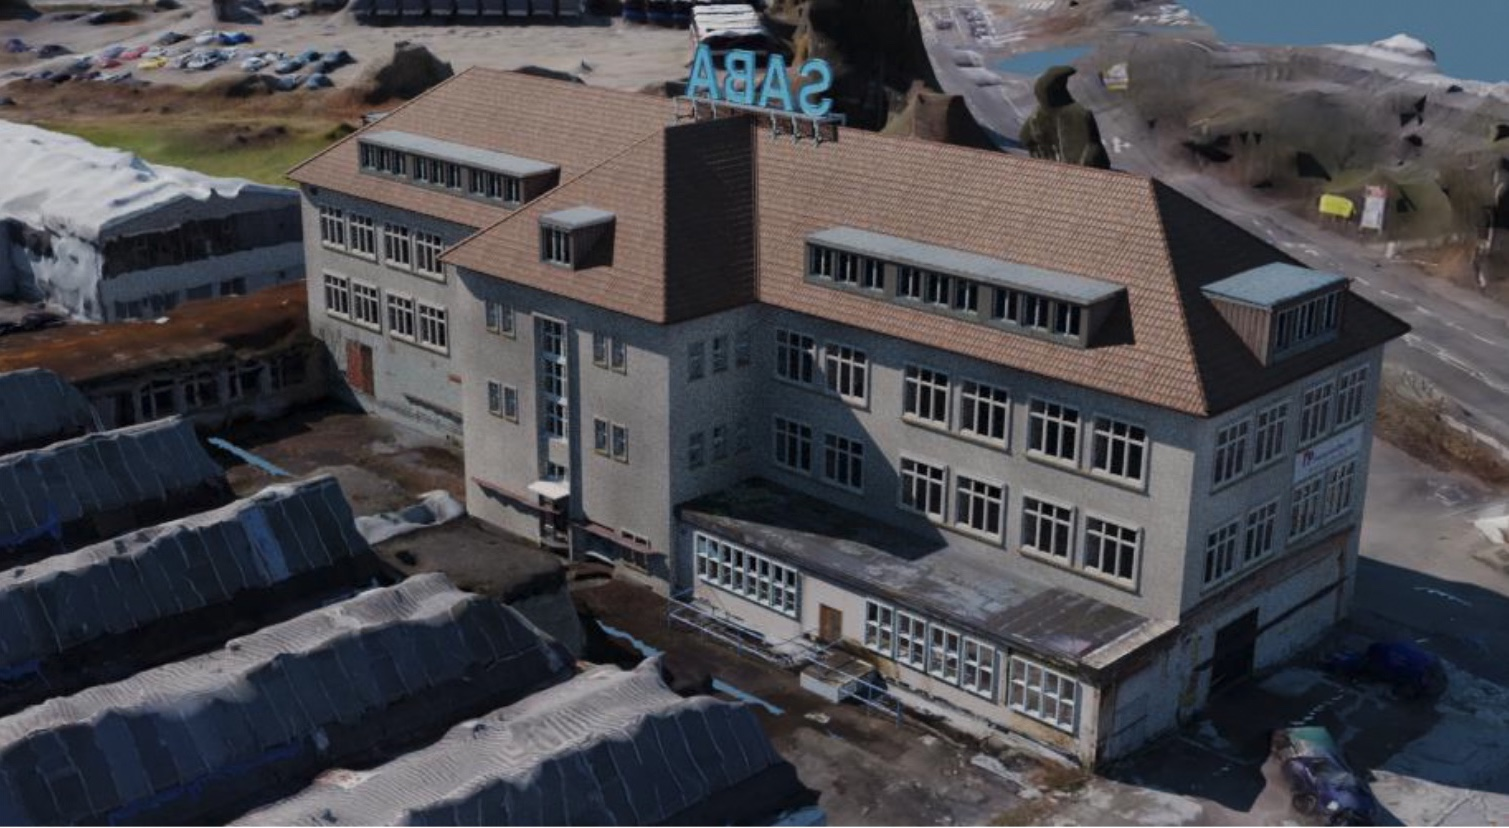
\includegraphics[width=0.6\textwidth]{vorangegangene_Projekte/saba_modell.jpg}
    \caption{Das 3D Modell des SABA Hauptgebäudes in der 3D Karte aus den Drohnen-Aufnahmen.}
    \label{fig:SABA3DModell}
\end{figure}

\subsubsection{Photogrammetrische Aufzeichnungen des Lyautey Geländes}
Im Projekt \textit{NISABA} \cite{nisaba2021} aus dem Sommersemester 2020 und Wintersemester 2020/21 sind 3D Modelle von Gebäuden des ehemaligen Lyautey Kasernengeländes (das heutige "Richthofen") entstanden. Auch in diesem Projekt werden verschiedene Photogrammetrie Programme genutzt. \textit{Meshroom}, \textit{Pix4DMapper} \footnote{https://www.pix4d.com/de/produkt/pix4dmapper-photogrammetrie-software}, \textit{Agisoft Metashape} \footnote{https://www.agisoft.com/} und \textit{WebODM} \footnote{https://www.opendronemap.org/webodm/} weden für dieses Projekt verwendet. Gute Ergebnisse erzielt dabei \textit{Pix4DMapper}, da viele Einstellungen über den Detailgrad getroffen und mehrere Projekte kombiniert werden können. Aus dem generierten Mesh wird auch hier eine Nachmodellierung in \textit{Blender} durchgeführt.

Das Lyautey Gelände umfasst insgesamt sieben Gebäude. Für jedes Gebäude gibt es ein fertiges Modell aus \textit{Pix4DMapper} und ein Modell, bei dem die Polygone reduziert sind. Nur das Manschaftsgebäude gibt es nachmodelliert. Das ist das Gebäude 4 in der Abbildung \ref{fig:lyautey-map}. Alle 3D Modelle können auf der Website des \textit{NISABA}-Projekts \footnote{https://nisaba.villingen-schwenningen.de/uebersicht/} begutachtet werden. 

\begin{figure}[h]
    \centering
    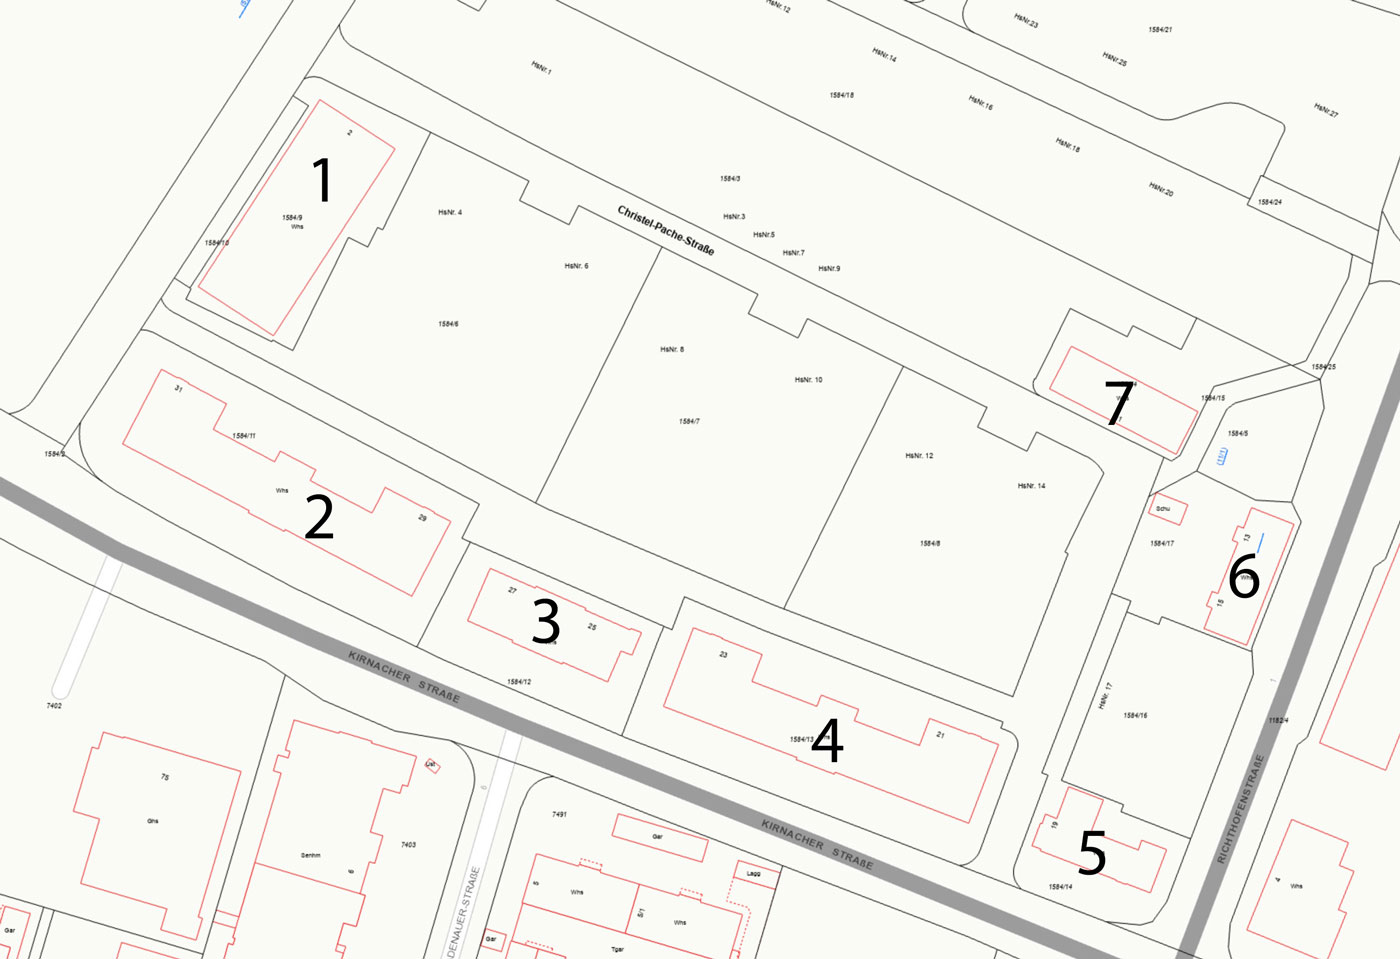
\includegraphics[width=0.8\textwidth]{img/vorangegangene_Projekte/lyautey_map.jpg}
    \caption{Eine Übersicht der Gebäude auf dem Lyautey-Gelände.}
    \label{fig:lyautey-map}
\end{figure}

\subsubsection{Photogrammetrische Aufzeichnungen des Mangin Geländes}
Im Zuge der Veranstaltung Bildverarbeitung und Computergrafik im Sommersemester 2021 im Studiengang Medieninformatik Master sind weitere 3D Modelle entstanden\cite{kusch2021}. Die Gebäude befinden sich auf dem für die Stadt historisch wichtigen Kasernengelände Mangin in Villingen-Schwenningen, das sich direkt östlich vom Lyautey befindet. Dabei handelt es sich um ein verlassenes Kasernengelände mit architektonisch und historisch interessanten Gebäuden. Die Aufnahmen der Gebäude erfolgte in Zusammenarbeit mit dem Vermessungsamt Villingen-Schwenningen. Es wurden Aufnahmen von den Gebäuden 2-8 und 10-12 gefertigt. In der Abbildung x ist eine Übersichtskarte des Geländes mit Nummerierungen der Gebäude zu sehen.  Die Bilder aus der Luft wurden mit einer Drohne vom Vermessungsamt gemacht, während die Aufnahmen am Boden von den Studierenden aufgenommen wurden. Als Photogrammetrie-Software wird hauptsächlich \textit{Pix4DMapper} und \textit{Meshroom} verwendet. 

\begin{figure}[h]
    \centering
    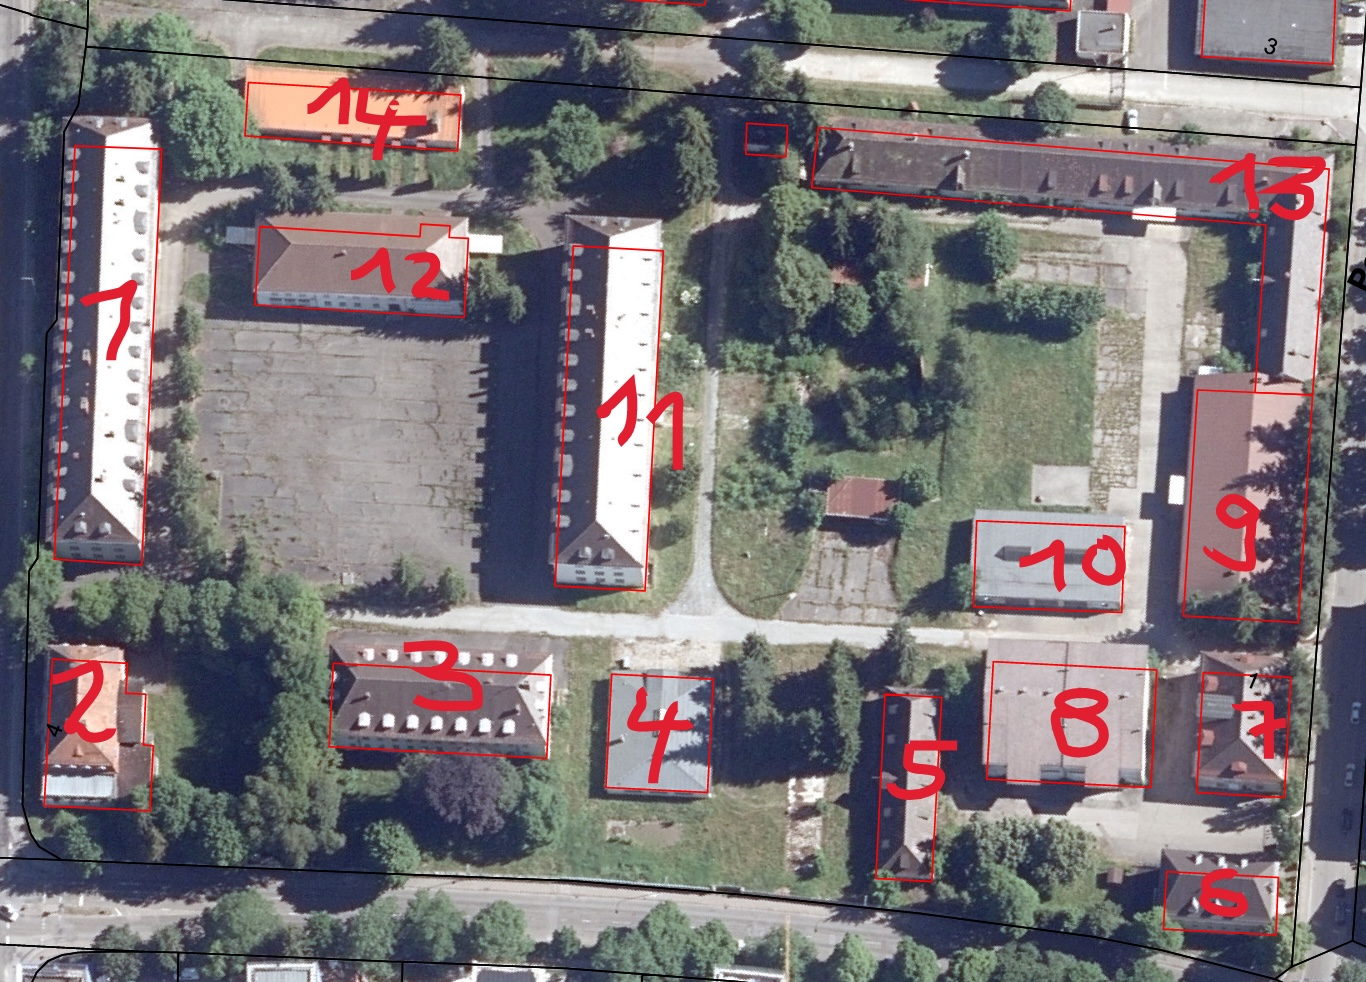
\includegraphics[width=0.8\textwidth]{img/vorangegangene_Projekte/mangin_map.jpg}
    \caption{Eine Übersicht der Gebäude auf dem Mangin-Gelände.}
    \label{fig:mangin-map}
\end{figure}
\subsubsection{Übersicht vorhandener 3D Modelle}
Einige Modelle sind nicht vollständig, haben aufgrund der Vegetation vor Ort Löcher im Mesh oder einen niedrigen Detailgrad. Daher können in dieser Arbeit nicht alle 3D Modelle verwendet werden. Die Tabelle \ref{tab:uebersicht-3Dmodelle} zeigt eine Liste der vorhandenen 3D Modelle. Die Gebäude sind wie in den Übersichtskarten nummeriert. Ein geringer Detailgrad bedeutet, dass das Mesh Löcher hat oder unvollständig ist. Ein mittlerer Detailgrad zeichnet sich durch ein vollständiges Mesh mit geringen Details aus. Gebäude mit einen hohen Detailgrad können für die \Gls{ar} Anwendung genutzt werden. Händisch modellierte Gebäude haben einen sehr hohen Detailgrad.
\begin{table}[h]
    \centering
    \begin{tabular}{|p{0.1\textwidth}|p{0.25\textwidth}|p{0.04\textwidth}|p{0.15\textwidth}|p{0.1\textwidth}|p{0.17\textwidth}|}
    \hline
        Gelände & Bezeichnung                                   & Nr.   & Detailgrad    & Vertices   & Texturenanzahl   \\ \hline 
        SABA    & Karte                                         & -     & gering        & 458.311    & 1                \\ \hline
        SABA    & Hauptgebäude \newline Neumodellierung         & 1     & sehr hoch     & 44.708     & 34               \\ \hline
        SABA    & Heizwerk                                      & 2     & mittel        & 142        & 8                \\ \hline
        Lyautey & Karte                                         & -     & mittel        & 2.049.590  & 1                \\ \hline
        Lyautey & Reithalle                                     & 1     & hoch          & 1.386.531  & 1                \\ \hline
        Lyautey & Mannschaftsgebäude 1                          & 2     & hoch          & 1.255.734  & 1                \\ \hline
        Lyautey & Wirtschaftsgebäude                            & 3     & hoch          & 1.610.983  & 1                \\ \hline
        Lyautey & Mannschaftsgebäude 2                          & 4     & hoch          & 175.352    & 1                \\ \hline
        Lyautey & Mannschaftsgebäude 2 \newline Neumodellierung & 4     & sehr hoch     & 2.046      & 45               \\ \hline
        Lyautey & Stabshaus                                     & 5     & gering        & -          & -                \\ \hline
        Lyautey & Familienhaus                                  & 6     & mittel        & 119.574    & 1                \\ \hline
        Lyautey & Kammergebäude                                 & 7     & hoch          & 269.460    & 1                \\ \hline
        Mangin  & Karte                                         & 1     & mittel        & 502.040    & 1                \\ \hline
        Mangin  & Casino                                        & 2     & mittel        & 681.082    & 1                \\ \hline
        Mangin  & -                                             & 3     & hoch          & 381.633    & 1                \\ \hline
        Mangin  & Pferdestall                                   & 4     & mittel        & 242.984    & 1                \\ \hline
        Mangin  & -                                             & 6     & gering        & 500.463    & 1                \\ \hline
        Mangin  & -                                             & 7     & gering        & 31.490     & 1                \\ \hline
        Mangin  & -                                             & 8     & hoch          & 5.093      & 1                \\ \hline
        Mangin  & -                                             & 10    & hoch          & 500.307    & 1                \\ \hline
        Mangin  & -                                             & 11    & mittel        & 427.753    & 1                \\ \hline
        Mangin  & -                                             & 12    & mittel        & 497.625    & 1                \\ \hline
        Mangin  & -                                             & 17    & gering        & 5.179      & 1                \\ \hline
        Mangin  & -                                             & 23    & gering        & 998        & 1                \\ \hline
        Mangin  & Karte der Gebäude 17-23                       & -     & mittel        & 15.433     & 1                \\ \hline
    \end{tabular}
    \caption{Eine Übersicht der vorhandenen 3D Modelle.}
    \label{tab:uebersicht-3Dmodelle}
\end{table}



% KAPITEL 2 Theoretische Grundlagen / Forschungsstand
% WICHTIG: Warum braucht der leser die Informationen, um die Arbeit zu verstehen?
% Einordnung AR
\section{Theoretische Grundlagen}
\subsection {Einordnung VR, AR und MR}
%Was ist AR
Bei Augmented Reality (\acrshort{ar}) Anwendungen werden dreidimensionale virtuelle Objekte in eine echte dreidimensionale Umgebung in Echtzeit integriert. Es handelt sich um eine Variation der Virtual Environments (\acrshort{ve}), der Virtuellen Realität (\acrshort{vr}) \cite{Azuma1997}. Gerne wird zwischen \acrshort{ar}, \acrshort{vr} und Mixed Reality (\acrshort{mr}) unterschieden. Speicher und seine Ko-Autoren \cite*{Speicher2019} haben zur Eingrenzung Charakteristiken definiert, die aus Interviews mit Experten hervorgehen. 

%VR
\acrshort{vr} hat die Eigenschaft eine komplett synthetisch generierte, virtuelle Welt darzustellen. So bietet sich die Möglichkeit für den Nutzer unerreichbare Orte zu erleben. Es werden hierfür VR-Headsets wie die Oculus Rift S\footnote{https://www.oculus.com/rift-s/, zuletzt aufgerufen am 27.07.2022} oder die Playstation VR\footnote{https://www.playstation.com/de-de/ps-vr/, zuletzt aufgerufen am 27.07.2022} benötigt und die Bewegung des Headsets muss getrackt\footnote{siehe Kapitel \ref{tracking} \nameref{tracking}} werden. Der Nutzer ist während der VR-Erfahrung von der echten Umgebung isoliert, wodurch die soziale Interaktion gering ist. 

%AR
Zusätzlich zu der Definition Azumas\cite{Azuma1997} von \acrshort{ar} wird die Eigenschaft genannt, dass der virtuelle Content dazu in der Lage ist mit der echten Welt zu interagieren. Im Gegensatz zu \acrshort{vr} ist der Nutzer im gegenwärtigen physischen Raum gebunden. Die menschliche Wahrnehmung wird durch das augmentieren und der Kreation von Content Erfahrungen verbessert\cite{Speicher2019}.

%MR
Die Eingrenzung von \acrshort{mr} ist nicht eindeutig. So wird \acrshort{mr} als Kombination von AR und VR gesehen. Die Anwendungen bieten die Möglichkeit sowohl AR als auch VR zu nutzen. Auch wird Mixed Reality in Verbindung mit spezifischer Hardware wie die HoloLens\footnote{https://www.microsoft.com/de-de/hololens, zuletzt aufgerufen am 27.07.2022} gebracht. Ein weiteres Beispiel ist Pokemon GO\footnote{https://pokemongolive.com/de/, zuletzt aufgerufen am 27.07.2022}, bei dem zwischen der AR Funktion und einer virtuellen Umgebung umgeschaltet werden kann.

In Abbidldung \ref*{fig: RV_Kontinuum} haben Milgram und seine Ko-Autoren eine Grafik definiert, die das \textit{Reality-Virtuality Continuum} darstellt. Die linke Hälfte des Kontinuums repräsentiert jede Umgebung, die rein aus realen Objekten besteht, persönlich betrachtet wird und durch jegliche Art wie den Blick durch ein Fenster oder eines Displays erweitert wird. Die rechte Hälfte besteht aus rein virtuellen Objekten, die entweder Monitor-basierend oder immersiv sind. Durch diese Darstellung wird \acrshort{mr} zwischen diesen beiden Extremen eingeordnet und als Umgebung definiert, die die reale und die virtuelle Welt zusammen in einem Display darstellt \cite{Milgram1995}.

\begin{figure}[H]
    \centering
    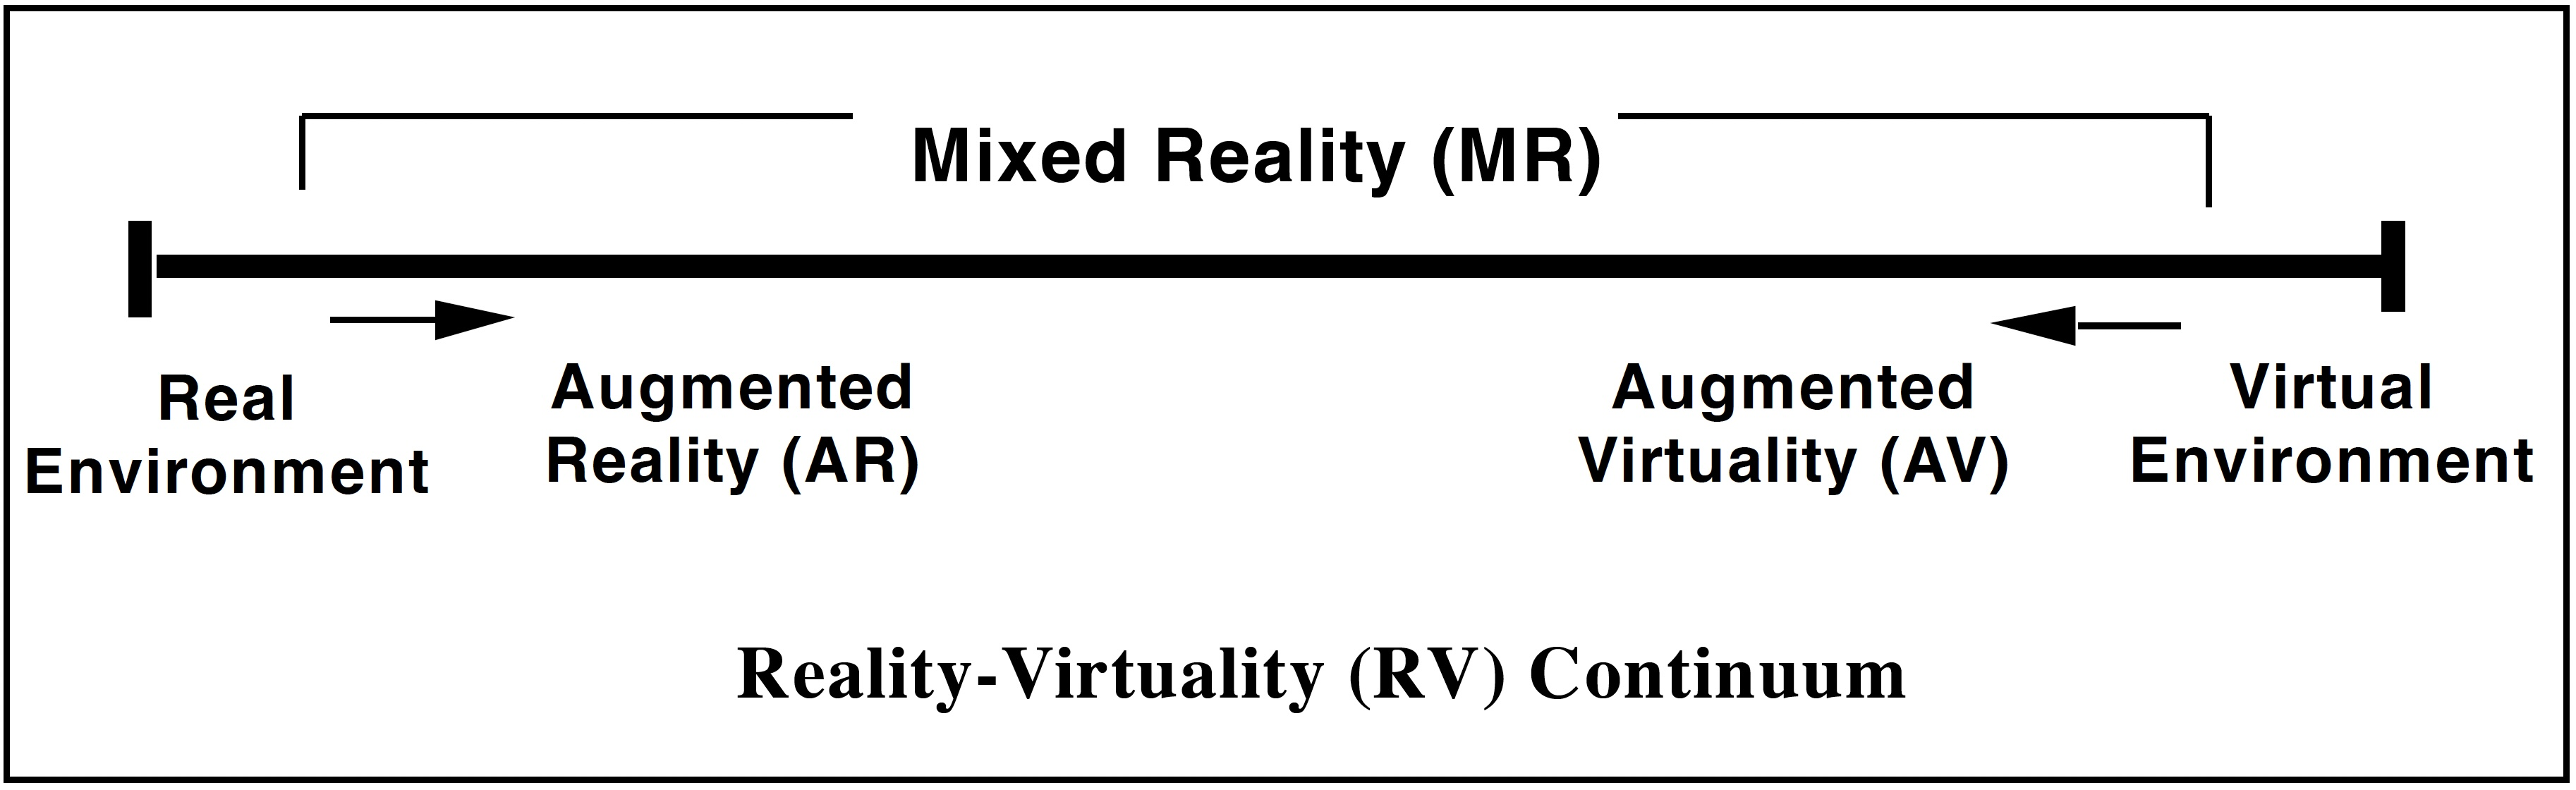
\includegraphics[width=\textwidth]{img/einordnung_vr_ar_mr/vr_ar_mr_kontinuum.jpg}
    \caption{Das Reality-Virtuality Kontinuum nach Milgram\cite{Milgram1995}.}
    \label{fig: RV_Kontinuum}
\end{figure}

Nach diesen Definitionen wird die Anwendung dieser Arbeit in die Augmented Reality eingeordnet. Die virtuellen Objekte in Form der Gebäude werden in die echte dreidimensionale Welt projiziert. Der Nutzer hat die Möglichkeit mit diesen zu interagieren. Jedoch wird es nicht möglich sein den betrachteten Raum zu verlassen und in eine reine virtuelle Welt umzusteigen. 

% Immersion Kriterien
%\section{Theoretische Grundlagen}
\subsection {Einordnung VR, AR und MR}
%Was ist AR
Bei Augmented Reality (\acrshort{ar}) Anwendungen werden dreidimensionale virtuelle Objekte in eine echte dreidimensionale Umgebung in Echtzeit integriert. Es handelt sich um eine Variation der Virtual Environments (\acrshort{ve}), der Virtuellen Realität (\acrshort{vr}) \cite{Azuma1997}. Gerne wird zwischen \acrshort{ar}, \acrshort{vr} und Mixed Reality (\acrshort{mr}) unterschieden. Speicher und seine Ko-Autoren \cite*{Speicher2019} haben zur Eingrenzung Charakteristiken definiert, die aus Interviews mit Experten hervorgehen. 

%VR
\acrshort{vr} hat die Eigenschaft eine komplett synthetisch generierte, virtuelle Welt darzustellen. So bietet sich die Möglichkeit für den Nutzer unerreichbare Orte zu erleben. Es werden hierfür VR-Headsets wie die Oculus Rift S\footnote{https://www.oculus.com/rift-s/, zuletzt aufgerufen am 27.07.2022} oder die Playstation VR\footnote{https://www.playstation.com/de-de/ps-vr/, zuletzt aufgerufen am 27.07.2022} benötigt und die Bewegung des Headsets muss getrackt\footnote{siehe Kapitel \ref{tracking} \nameref{tracking}} werden. Der Nutzer ist während der VR-Erfahrung von der echten Umgebung isoliert, wodurch die soziale Interaktion gering ist. 

%AR
Zusätzlich zu der Definition Azumas\cite{Azuma1997} von \acrshort{ar} wird die Eigenschaft genannt, dass der virtuelle Content dazu in der Lage ist mit der echten Welt zu interagieren. Im Gegensatz zu \acrshort{vr} ist der Nutzer im gegenwärtigen physischen Raum gebunden. Die menschliche Wahrnehmung wird durch das augmentieren und der Kreation von Content Erfahrungen verbessert\cite{Speicher2019}.

%MR
Die Eingrenzung von \acrshort{mr} ist nicht eindeutig. So wird \acrshort{mr} als Kombination von AR und VR gesehen. Die Anwendungen bieten die Möglichkeit sowohl AR als auch VR zu nutzen. Auch wird Mixed Reality in Verbindung mit spezifischer Hardware wie die HoloLens\footnote{https://www.microsoft.com/de-de/hololens, zuletzt aufgerufen am 27.07.2022} gebracht. Ein weiteres Beispiel ist Pokemon GO\footnote{https://pokemongolive.com/de/, zuletzt aufgerufen am 27.07.2022}, bei dem zwischen der AR Funktion und einer virtuellen Umgebung umgeschaltet werden kann.

In Abbidldung \ref*{fig: RV_Kontinuum} haben Milgram und seine Ko-Autoren eine Grafik definiert, die das \textit{Reality-Virtuality Continuum} darstellt. Die linke Hälfte des Kontinuums repräsentiert jede Umgebung, die rein aus realen Objekten besteht, persönlich betrachtet wird und durch jegliche Art wie den Blick durch ein Fenster oder eines Displays erweitert wird. Die rechte Hälfte besteht aus rein virtuellen Objekten, die entweder Monitor-basierend oder immersiv sind. Durch diese Darstellung wird \acrshort{mr} zwischen diesen beiden Extremen eingeordnet und als Umgebung definiert, die die reale und die virtuelle Welt zusammen in einem Display darstellt \cite{Milgram1995}.

\begin{figure}[H]
    \centering
    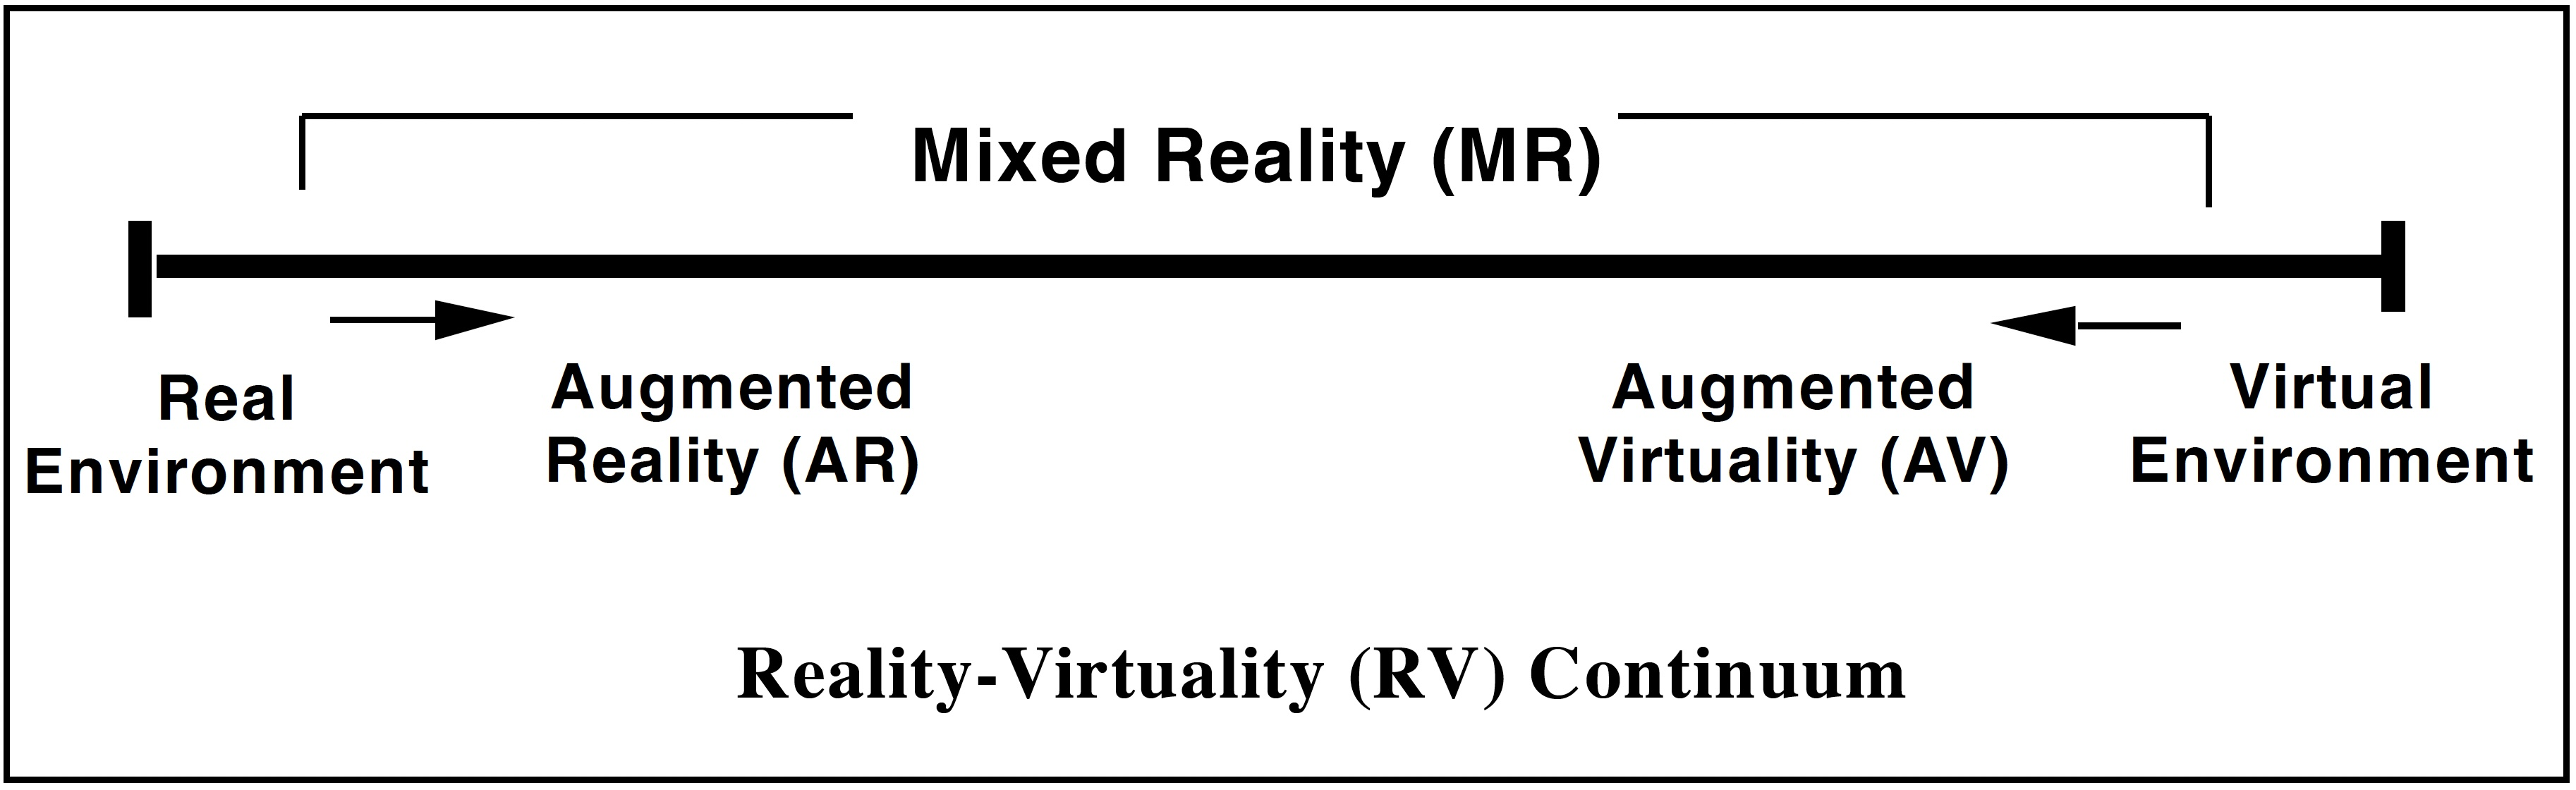
\includegraphics[width=\textwidth]{img/einordnung_vr_ar_mr/vr_ar_mr_kontinuum.jpg}
    \caption{Das Reality-Virtuality Kontinuum nach Milgram\cite{Milgram1995}.}
    \label{fig: RV_Kontinuum}
\end{figure}

Nach diesen Definitionen wird die Anwendung dieser Arbeit in die Augmented Reality eingeordnet. Die virtuellen Objekte in Form der Gebäude werden in die echte dreidimensionale Welt projiziert. Der Nutzer hat die Möglichkeit mit diesen zu interagieren. Jedoch wird es nicht möglich sein den betrachteten Raum zu verlassen und in eine reine virtuelle Welt umzusteigen. 

% Tracking
\subsection{Tracking}
\label{tracking}
Die Bewegung eines starren Körpers wird mit drei Koordinaten für die Position und drei Winkeln für die Orientierung angegeben\cite*[Dörner (2019) S.119f.,][]{doerner}. Diese sechs Werte werden als \textit{Freiheitsgrade (engl. \acrfull{dof})} bezeichnet. Der Begriff Tracking beschreibt die kontinuierliche Verfolgung von Positions- und Orientierungsdaten.

Im AR Kontext wird die Position und Orientierung des Smartphones kontinuierlich berechnet. Gleichzeitig wird die Umgebung erfasst und sogenannte Schlüsselpunkte festgelegt. Anhand der Schlüsselpunkte können z.B. Flächen erkannt werden, auf denen die virtuellen Objekte platziert werden. Billinghurst\cite[][]{billinghurst2015} nennt zwei Phasen beim Tracking:

\begin{itemize}
    \item eine Registrierungsphase, bei der die Position und Orientierung des Smartphones beim Start der Anwendung im Bezug auf einem Ankerpunkt in der realen Welt bestimmt wird,
    \item eine Trackingphase, bei der die Position und Orientierung des Smartphones anhand der vorherigen Position und Orientierung aktualisiert wird.
\end{itemize}

Das Ziel beim Tracking ist es, die sechs Freiheitsgrade für die Translation und Rotation der Objekte kontinuierlich zu bestimmen bzw. zu schätzen. Die Aufnahme der Daten erfolgt durch Sensoren z.B. durch die \textit{\acrfull{imu}} in Smartphones und Tablets. Die IMU wird in Kapitel \ref*{tracking-imu} behandelt.

Es werden zwischen zwei Trackingverfahren unterschieden. Beim \textit{Outside-In-Tracking} befindet sich die Sensorik zur Datenaufnahme in der Umgebung innerhalb eines bestimmten Raumes, sodass das Objekt von außen getrackt wird. Dies wird bei VR-Brillen eingesetzt. Der Nachteil dieser Technik ist, dass die Sensoik an einem Ort gebunden ist und bei einem Ortswechsel neu platziert werden muss. Beim \textit{Inside-Out-Tracking} befinden sich Sensoren im Objekt, das getrackt werden soll. Die Position und Lage des Objekts wird im Verhältnis zur Umgebung gesetzt. Bei der AR Anwendung in dieser Arbeit handelt es sich somit um ein Inside-Out-Tracking. Vorteil dieser Methode ist, dass der Nutzer nicht an einem Ort gebunden ist. Probleme treten in der Genauigkeit beim Tracking auf. Das Tracking System im Smartphone muss sich rein auf die Sensoren in der IMU und dem Kamerabild verlassen, während beim Outside-InTracking mehr Sensoren zur Verfügung stehen.

In der Unity Manual zu AR Foundation wird der Begriff Tracking mit der Bestimmung der relativen Position und Orientierung in der physichen Welt definiert. Zusätzlich wird darauf hingewiesen, dass falls die Umgebung zu dunkel ist, das Gerät Probleme beim Tracking bekommt und die Genauigkeit der Positionsbestimmung sich verringert \cite{UnityARFoundation}. Damit ist davon auszugehen, dass in AR Foundation Kamera-basiertes Tracking (siehe Kapitel \ref*{tracking-kamerabasiertes-tracking}) verwendet wird. Kamera-basiertes Tracking wird in Kapitel \ref*{tracking-kamerabasiertes-tracking} näher behandelt.

\subsubsection{Koordinatensysteme}
\label{tracking-koordinatensysteme}
Um eine Bestimmung bzw. Schätzung der Translationen und Rotationen durchzuführen, werden zwei Koordinatensysteme herangezogen. Ein Kamerakoordinatensystem und ein Objektkoordinatensystem. Weiterhin gibt es die Möglichkeit, dass für alle Objekte im Raum ein Koordinatensystem (Weltkoordinatensystem) verwendet wird. Voraussetzung für das Tracking ist, dass die Transformationen zwischen den Objekten bekannt sind. Dann kann die Transformation zwischen dem Objekt und dem Weltkoordinatensystem geschätzt werden.\cite*[Dörner (2019) S.124f.,][]{doerner}.

In Unity und AR Foundation hat das Smartphone ein eigenes Koordinatensystem. Wird eine AR-Session gestartet, so wird ein Koordinatensystem für diese spezifische Session initialisiert. Die Koordinaten (0,0,0) stehen für die Position des Gerätes, bei dem die Session gestartet ist \cite{UnityARFoundation}. Die z-Achse zeigt dabei in die Richtung, in die die Kamera des Smartphones gerichtet ist. Dieser Umstand ist für die Roatation der Gebäude in der GPS Platzierung relevant und wird in Kapitel \ref*{umsetzung-gps-ausrichtung-nach-norden} erläutert. Die \textit{GameObjects} in der Szene haben ein lokales Objektkoordinatensystem.

\subsubsection{Tracking mit der Inertial Measurement Unit (IMU)}
\label{tracking-imu}
Eine Inertial Measurement Unit besteht typischerweise aus Beschleungungssensoren, Drehratensensoren. Drei Beschleunigungssensoren und drei Drehratensensoren werden orthogonal zueinander eingebaut. Die Sensoren bilden ein Trägheitsnavigationssystem. Dieses misst die Bewegungsrichtung, die Beschleunigung und die Drehung in einem kartesischen Koordinatensystem und bestimmt damit die Position und Orientierung der \acrshort{imu}\footnote{https://www.5gpositioning.com/inertial-measurement-units-in-smartphones/, zuletzt aufgerufen am 27.07.2022}. Die Orientierung kann anhand der Drehratensensoren präzise bestimmt werden. Die Position wird mit den Beschleunigungswerten und der dabei vergangenen Zeit pro Aktualisierung berechnet. Die Genauigkeit dieser Berechnung ist insbesondere bei niedrigpreisigen Smartphones nicht akkurat. Es kommt zu \textit{Drifteffekten}.
Dörner beschreibt den Hintergrund des Probelms präzise: 

\glqq [..] wird beispielsweise ein Sensor aus dem Ruhezustand bewegt und anschließend wieder angehalten, so müssten sowohl die Summen der erfassten Beschleunigungswerte wie auch die der errechneten Geschwindigkeitswerte am Ende Null ergeben\grqq{}\cite*[Dörner (2019) S.127f.,][]{doerner}. 
Durch die Ungenauigkeit wird dies nicht erzielt und die errechnete Position weicht von der tatsächlichen Position ab. Zur Bestimmung der Orientierung wird die IMU oft genutzt. Da in AR Anwendungen eine hohe Präzision in der Positionsbestimmung benötigt wird, wird reines IMU-Tracking nicht genutzt. Es wird zusätzliche Kamera-basiertes Tracking benötigt, um den Drifteffekt auszugleichen\cite[Billinghurst (2015),][]{billinghurst2015}.

\subsubsection{Kamera-basiertes Tracking}
\label{tracking-kamerabasiertes-tracking}
Kamera-basiertes Tracking nutzt Bilder, um die relative Position und Orientierung der Objekte zur Kamera zu bestimmen. Die Position und Orientierung der Kamera in einem Weltkoordinatensystem wird von Hartley und Zisserman als extrinsische Kameraparameter bezeichnet \cite*[Hartley, Zisserman (2003) S.156,][]{hartleyzisserman}. Für das Kamera-basierte Tracking wird zwischen Marker-basierten und Marker-less Tracking unterschieden.

Beim Marker-basierten Tracking werden Marker (sogenannte Kanji und Hiro Marker) wie in Abbildung \ref{fig: tracking_kanji_hiro} zu sehen genutzt. Billinghurst\cite[][]{billinghurst2015} bezeichnet dies als \textit{Fiducial Tracking}. Dabei werden künstliche Marker in der Umgebung platziert. Sie dienen als Ursprung, sodass diese als als Orientierungshilfen fungieren. Populär wurde die Methode durch ARToolkit, das von Kato und Billinghurst\cite[(1999),][]{kato1999} entwickelt wurde. Das jeweilige Muster und die Größe der Marker müssen für das Tracking bekannt sein. Der Tracking Prozess ist in Abbildung \ref*{fig: tracking_ARToolkit} zu sehen. Zunächst wird das Bild im Videodatenstrom binarisiert. Die Ränder des Markers werden identifiziert. Anschließend wird die Position und die Orientierung relativ zur Kamera berechnet. Die Symbole im Marker werden mit den bekannten Symbolen aus der Datenbank verglichen und gematched. Letzlich wird  das virtuelle Objekt mit der Position und Orientierung des Markers transformiert und in das Kamerabild gerendert.

\begin{figure}[H]
    \centering
    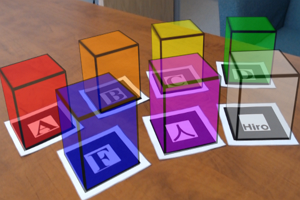
\includegraphics[width=7cm]{img/tracking/kanjo-hiro-marker.png}
    \caption[Kanji und Hiro Marker haben einfache geometrische Formen, Texte oder Buchstaben zur Erkennung in der Szene.]{Kanji und Hiro Marker haben einfache geometrische Formen, Texte oder Buchstaben zur Erkennung in der Szene\protect\footnotemark.}
    \label{fig: tracking_kanji_hiro}
\end{figure}
\footnotetext{Quelle Bild: https://stemkoski.github.io/AR-Examples/, zuletzt aufgerufen am 29.07.2022}
\begin{figure}[H]
    \centering
    \includegraphics[width=\textwidth]{img/tracking/tracking-ARToolkit.jpg}
    \caption{Der Tracking Prozess von ARToolkit\cite*[Billinghurst(2015),][]{billinghurst2015}.}
    \label{fig: tracking_ARToolkit}
\end{figure}

Die Methode ist simpel und bietet eine hohe Genauigkeit beim Tracking. Da die Marker aktiv in der Umgebung platziert werden müssen, gibt es Einschränkungen in der Flexibilität. Daher wird bei der zweiten Möglichkeit über Algorithmen der Computer Vision Merkmale in der realen Umgebung erfasst. Dies wird als \textit{marker-less AR} bezeichnet. Diese Merkmale sind Punkte oder Ecken, die aus der Umgebung herausstechen und als einzigartigen Punkt gelten. Sie sind natürliche Marker in der Umgebung. In den folgenden Kapiteln werden natürliche Merkmals-Detektoren benannt und deren Funktionsweise anhand des \acrfull{sift} Algorithmus erklärt.

\subsubsubsection{Schlüsselpunkte detektieren (Feature Detection)}
Merkmale oder auch \textit{keypoint features} oder \textit{interest points} sind Bildbereiche mit einem zentralen Punkt, die einen hohen Wiedererkennungswert besitzen. In Abbildung \ref*{fig: tracking_feature_detection_prinzip} wird deutlich, dass Flächen ohne Texturen schwer identifiziert und abgeglichen werden können. Dieses Problem ist als \textit{aperture Problem} bekannt. Erst durch starke Kontraständerungen an der Richtung der Normalen zur Kante\footnote{die durch Gradienten erkannt werden. Ein Gradient bestimmt die Richtung und Steigung der größten Änderung.}, werden Merkmale erkannt\cite[Szeliski(2022) Seite 337f., ][]{szeliski2022}. 

\begin{figure}[H]
    \centering
    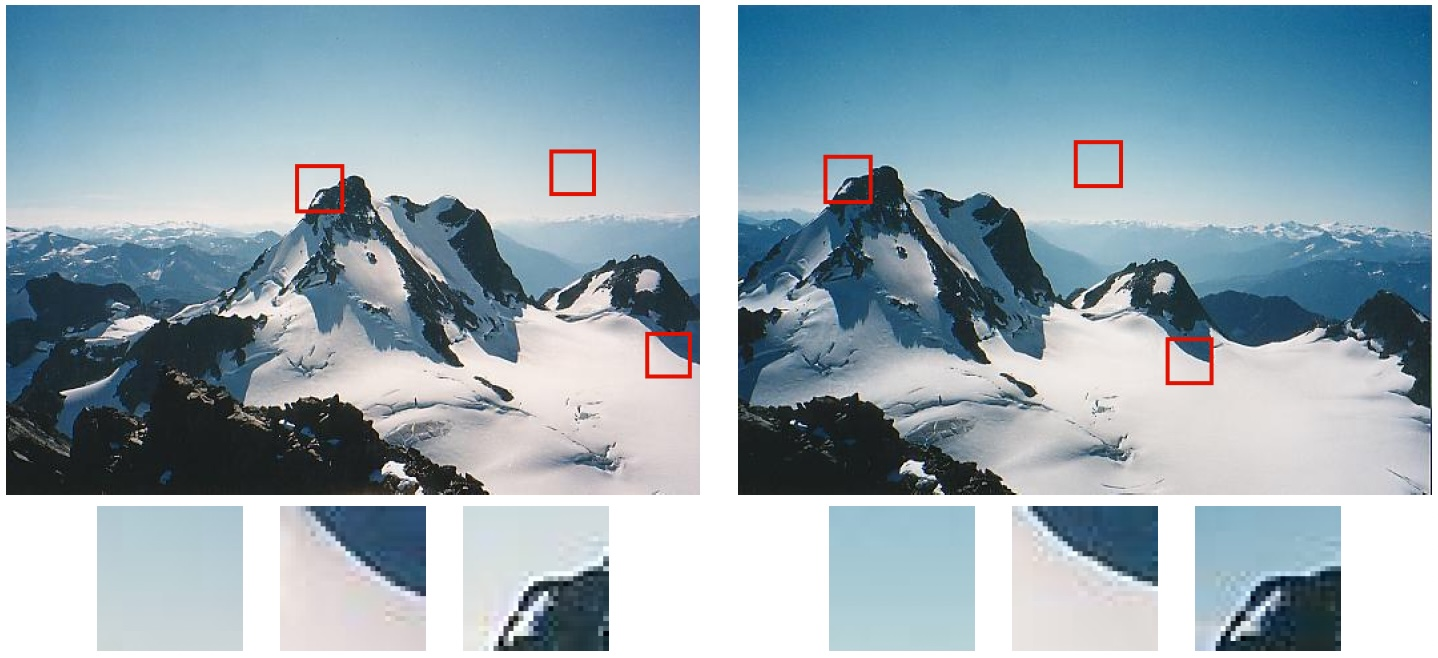
\includegraphics[width=\textwidth]{img/tracking/Feature-detection-problem.jpg}
    \caption[Die Wahrscheinlichkeit, dass eine Fläche aus dem linken Bild im rechten Bild genau identifiziert werden kann steigt, wenn starke Kontraständerungen (Gradienten) im Teilbild vorhanden sind.]{Die Wahrscheinlichkeit, dass eine Fläche aus dem linken Bild im rechten Bild genau identifiziert werden kann steigt, wenn starke Kontraständerungen (Gradienten) im Teilbild vorhanden sind\protect\footnotemark.}
    \label{fig: tracking_feature_detection_prinzip}
\end{figure}

\footnotetext{Quelle Bild: \cite*[Szeliski(2022) Seite 337,][]{szeliski2022}}

Es wird zwischen \textit{Eckendetektoren} und \textit{Blob Detektoren} unterschieden. Bekannte Kantendetektoren sind z.B.:
\begin{itemize}
    \item Harris\cite*{harris1988},
    \item \acrfull{fast} von Rosten und Drummond\cite[][]{rosten2005}.
\end{itemize}
Bekannte Blob-Detektoren sind z.B.:
\begin{itemize}
    \item \acrfull{sift} von Lowe\cite{lowe1999},
    \item \acrfull{surf} von Bay u.a.\cite{bay2008},
    \item \acrfull{orb} von Rublee u.a.\cite{rublee2011}.
\end{itemize}

Herling und Broll\cite{herling2011} nennen Herausforderungen für Detektoren, damit eine valide Position und Orientierung berechnet werden kann:
\begin{itemize}
    \item Da AR in Echtzeit abläuft, muss die Bestimmung von Schlüsselpunkten und Deskriptoren schnell berechnet werden,
    \item der Algorithmus muss robust gegenüber unterschiedlichen Lichtverhältnissen. Dies gilt insbesondere bei AR in freier Umgebung, da eine hohe Dynamik herrscht und die Lichtverhältnisse sich schnell verändern können,
    \item da der Nutzer keine Einschränkungen in der Position der Kamera besitzt, kann ein schneller Perspektivwechsel erfolgen. Der Algorithmus muss daher eine Robustheit genüber starken Bildveränderungen haben,
    \item es muss eine Skalierungsinvarianz bereitgestellt werden. Das bedeutet im \acrshort{ar} Kontext, dass das Tracking nicht auf eine bestimmte Entfernung beschränkt ist und weiter entfernte Punkte nicht verschwinden. In einem abgegrenzten Bereich ist es einfacher Schlüsselpunkte zu detektieren. Die Skaleninvarianz ist daher insbesondere bei \acrshort{ar} im Freien relevant, da hier die Umgebung unbegrenzt ist.
\end{itemize}

Die Blob Detektoren wählen Schlüsselpunkte aus, die einen fleckenartige Eigenschaft besitzen. Es sind z.B. Punkte oder große verschwommene Flächen, die ähnliche Farbintensitäten besitzen\cite[Herling und Broll(2011),][]{herling2011}. Im folgenden Abschnitt wird die Herangehensweise anhand des \acrshort{sift} Algorithmus erläutert.

Zunächst wird eine Gauss Pyramide gebildet. Dabei wird ein Eingangsbild verkleinert und in mehreren Durchläufen mit einem Gauss-Filter weichgezeichnet. Dann erfolgt eine weitere Skalierung und Gauss-Filter Ebene. Eine Ebene wird dabei \textit{Octave} genannt. Dieser Prozess ist in Abbildung \ref*{fig: tracking-gauss-pyramide} zu sehen und wird so lange durchgeführt, bis das Bild so klein ist, dass es nicht weiter verkleinert werden kann. Dadurch entsteht ein Skalenraum, der die Skaleninvarianz implementiert und das Bild in mehreren Skalierungen bereitstellt. Der Sinn dabei ist es, das Bild aus verschiedenen Entfernungen zu betrachten. So ist ein Baum aus der Entfernung durch seinen Aufbau als Feature zu erkennen. Ist der Baum im Bild groß skaliert, werden die Blätter des Baumes als Feature erkannt. Da die Detektoren keine Vorkenntnisse über das Bild haben, wird dieser Skalenraum erstellt. Der Gauss Filter wird benötigt, um feine Strukturen wie z.B. Bildrauschen oder zu feine Strukturen herauszufiltern. 

\begin{figure}[H]
    \centering
    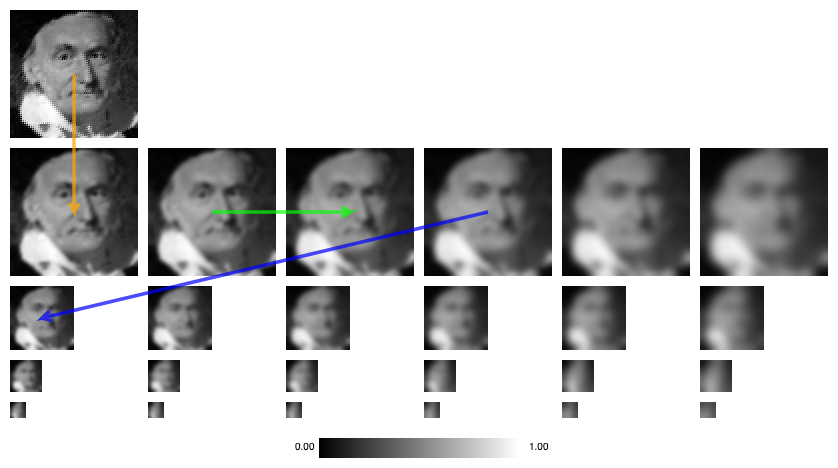
\includegraphics[width=\textwidth]{img/tracking/gauss-pyramide.png}
    \caption[Die Gauß-Pyramide für ein Eingangsbild. Das Bild wird runterskaliert und mit steigender Stärke mit einem Gauss-Weichzeichner versehen.]{Die Gauß-Pyramide für ein Eingangsbild. Das Bild wird runterskaliert und mit steigender Stärke mit einem Gauss-Weichzeichner versehen\protect\footnotemark.}
    \label{fig: tracking-gauss-pyramide}
\end{figure}

\footnotetext{Quelle Bild: http://weitz.de/sift/, zuletzt aufgerufen am 01.08.2022}

Dann werden nach \textit{Schlüsselpunkten (engl. Key Points, Feature Points)} in einem Bild gesucht. Es wird von je zwei benachbarten Bildern in der Gauß-Pyramide die Differenz gebildet (\textit{Difference of Gaussians (DoG)}). Dadurch entstehen Grauwerte, die diskrete Maximas erkennen lassen. Für jeden Punkt wird der Grauwert des mittleren Pixels mit den Grauwerten der umliegenden Pixel und die Grauwerte der benachbarten Bilder an der gleichen Stelle verglichen. Ist ein starker Unterschied bemerkbar, gilt der Punkt als Kanditat für einen Schlüsselpunkt. In Abbildung \ref*{fig:tracking-sift-features} werden Schlüsselpunkte gefunden. Die roten Punkte enthalten starke Extrema, die im weiteren Verlauf betrachtet werden. Die gelben Punkte enthalten zwar Extrema, jedoch sind die Unterschiede der Grauwerte so gering, dass sie unter dem eingestellten Schwellwert liegen und aussortiert werden. Diese werden beispielsweise als Rauschen erkannt. Je nachdem wie groß das Bild ist und wie stark die Schwellwerte beim jeweiligen Detektor eingestellt sind, verändert sich die Anzahl an Schlüsselpunkten. Dies beeinflusst die Tracking Performance und die Genauigkeit.
Wie?

\begin{figure}[H]
    \centering
    \subfloat[][]{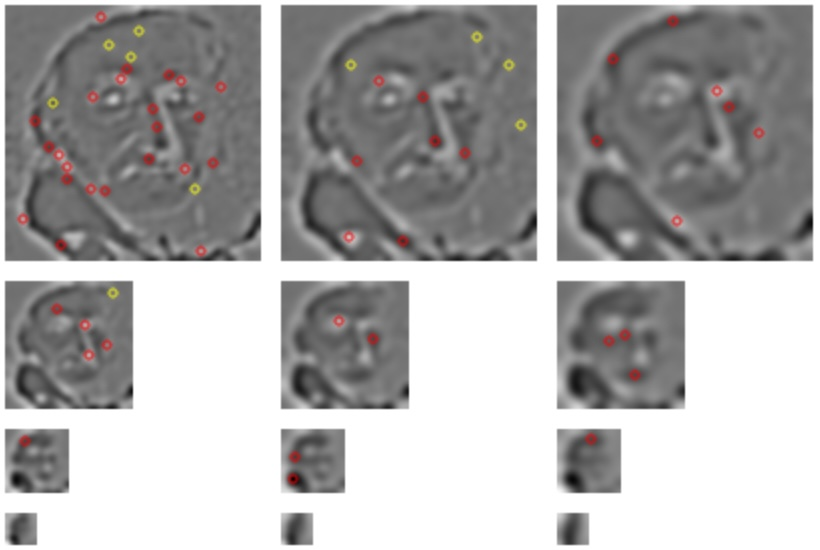
\includegraphics[width=0.4\linewidth]{img/tracking/feature-detection-sift.jpg}}%
    \qquad
    \subfloat[][]{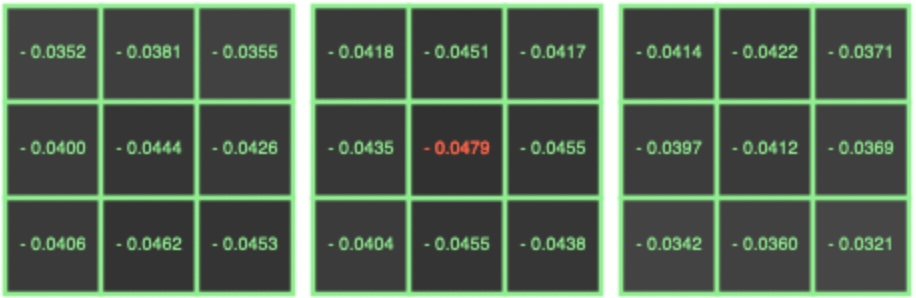
\includegraphics[width=0.4\linewidth]{img/tracking/feature-detection-sift-werte.jpg}}%
    \caption[Detektierte Schlüsselpunkte anhand der Extremas der DoG Bilder und deren Nachbarbilder (a) und die Grauwerte des Punktes auf der Nasenspitze der Person (b). Der Grauwert an der Stelle der Nase unterscheidet sich stark von seinen benachbarten Pixeln und beherbergt daher ein Extrema]{Detektierte Schlüsselpunkte anhand der Extremas der DoG Bilder und deren Nachbarbilder (a) und die Grauwerte des Punktes auf der Nasenspitze der Person (b). Der Grauwert an der Stelle der Nase unterscheidet sich stark von seinen benachbarten Pixeln und beherbergt daher ein Extrema\protect\footnotemark.}%
    \label{fig:tracking-sift-features}
\end{figure}

\footnotetext{Quelle Bild: http://weitz.de/sift/, zuletzt aufgerufen am 01.08.2022}

Nach der ersten Auswahl der Schlüsselpunkte wird die Positionen der Schlüsselpunkte verbessert. Dazu werden mit der Taylor-Formel Taylorpolynome gebildet. Diese werden in der Mathematik genutzt, Punkte in der Umgebung einer Funktion anzunähern\footnote{https://de.wikipedia.org/wiki/Taylor-Formel, zuletzt aufgerufen am 01.08.2022}. Mit den Polynomen werden die diskreten x- und y-Koordinaten durch Nachkommastellen verfeinert. Mit feineren Koordinaten wird der Punkt genauer erfasst und die Auswahl der Schlüsselpunkte wird ebenfalls verfeinert.

Ist eine finale Auswahl der Schlüsselpunkte erfolgt, erhält jeder Punkt einen sogenannten \textit{Deskriptor}. Dieser enthält lokale Eigenschaften auf dem Bild in der Umgebung des Punktes. Ziel eines Deskriptors ist es Schlüsselpunkte eindeutig zu beschreiben. Der Algorithmus nimmt jeden Schlüsselpunkt, berechnet in einem bestimmten viereckigen Bereich um den Punkt Gradienten. Ein Gradient bestimmt die Richtung und Steigung der größten Änderung\footnote{https://de.wikipedia.org/wiki/Gradient, zuletzt aufgerufen am 01.08.2022}. Die Gradienten werden in einem Histogramm gespeichert. Aus dem Histogramm wird ersichtlich, in welche Richtung die meisten Gradienten zeigen und es wird daraus eine Referenzrichtung dieses Punktes abgeleitet. Der gleiche Prozess wird im nächsten Schritt nochmals durchgeführt. Jetzt ist die Auswahl kreisförmig und das genutzte Koordinatensystem orientiert sich an der zuvor abgeleiteten Referenzrichtung. Es wird wieder eine Hauptrichtung der Gradienten bestimmt und die Gradienten werden in weitere Histogramme abgespeichert. Die Informationen sind dazu da, die Schlüsselpunkte rotationsinvariant zu machen \cite*[Herling und Broll(2011),][]{herling2011} \cite*[Weitz(2022),][]{weitz2022}. 

Der Deskriptor hat am Ende des Algorithmus folgende Informationen für jeden Schlüsselpunkt:

\begin{itemize}
    \item Die verfeinerten x- und y-Koordinaten,
    \item der Skalierungsfaktor,
    \item der Grad an Unschärfe,
    \item die Hauptrichtungen der Gradienten,
    \item normalisierte 4x4x8=128 8-bit integer Werte, die die Histogramme aus dem letzten Schritt darestellen.
\end{itemize}

Diese Informationen beschreiben jeden Schlüsselpunkt eindeutig. Der Punkt ist durch die Skalierungen skaleninvariant, wenig anfällig für Rauschen oder feine Strukturen und rotierungsinvariant.

\begin{figure}[H]
    \centering
    \subfloat[][]{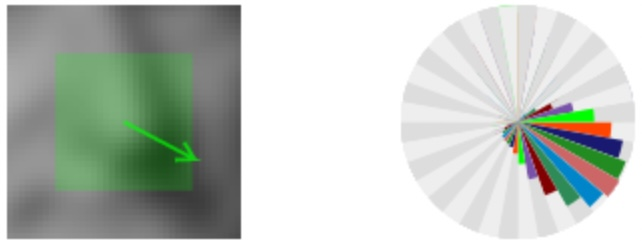
\includegraphics[width=0.4\linewidth]{img/tracking/feature-detection-sift-hauptrichtung.jpg}}%
    \qquad
    \subfloat[][]{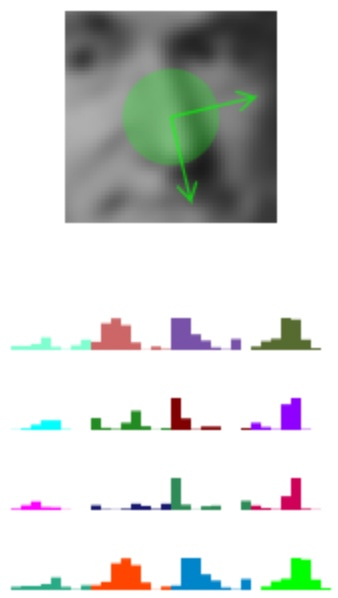
\includegraphics[width=0.4\linewidth]{img/tracking/feature-detection-histogramme.jpg}}%
    \caption[Das Histogramm und die Referenzrichtung im ersten Durchlauf (a) und das Koordinatensystem nach der Referenzrichtung und die entstandenen Histogramme(b).]{Das Histogramm und die Referenzrichtung im ersten Durchlauf (a) und das Koordinatensystem nach der Referenzrichtung und die entstandenen Histogramme(b)\protect\footnotemark.}%
    \label{fig:tracking-sift-richtungen}
\end{figure}

\footnotetext{Quelle Bild: http://weitz.de/sift/, zuletzt aufgerufen am 01.08.2022}

\subsubsubsection{Feature-Matching}

Sind die Deskriptoren vorhanden, kann im Anschluss ein \textit{Feature-Matching} durchgeführt werden. Dabei werden Schlüsselpunkte mit ihren Deskriptoren verglichen und zugeordnet. Mithilfe der zugeorndeten Schlüsselpunkten kann die Pose der Kamera berechnet werden \cite[Dörner(2019)][]{doerner}\cite[Herling und Broll(2011)][]{herling2011}. 

Als Beispiel wird mit Python\footnote{https://www.python.org/} und OpenCV\footnote{https://opencv.org/} ein Feature-Matching durchgeführt. Hierfür wird \acrshort{orb} verwendet. Abbildung \ref*{fig:orb-beispiel} zeigt das Feature-Matching Ergebnis mit der Brute Force Methode. Bei der Brute Force Methode werden die Deskriptoren verglichen. Der Deskriptor der, der am nächsten zum vergleichenden Deskriptor ist, wird zurückgegeben und als Match identifiziert\footnote{\url{https://docs.opencv.org/3.4/dc/dc3/tutorial_py_matcher.html}, zuletzt aufgerufen am 02.08.2022}. In diesem Beispiel wird die Skaleninvarianz und die Rotierungsinvarianz ersichtlich.

\begin{figure}[H]
    \centering
    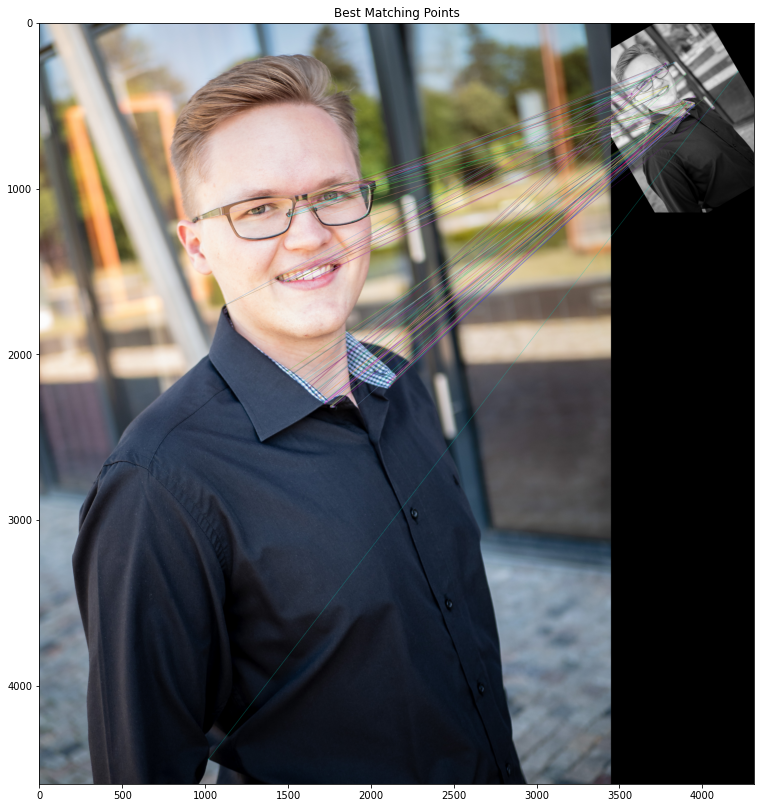
\includegraphics[width=10cm]{img/tracking/orb-3.png}
    \caption[Das Ergebnis des Feature-Matching mit ORB und OpenCV.]{Das Ergebnis des Feature-Matching mit ORB und OpenCV.\protect\footnotemark}
    \label{fig:orb-beispiel}
\end{figure}

\footnotetext{Link zum Source-Code:\\ \url{https://medium.com/data-breach/introduction-to-orb-oriented-fast-and-rotated-brief-4220e8ec40cf}, und das Beispiel: \url{https://github.com/Koliyoshii/masterarbeit/blob/main/opencv_orb_feature_matching.ipynb}}

\subsubsubsection{Simultaneous Localization and Mapping (SLAM)}
Während bei Feature-Matching Methoden eine Feature-Map für das Tracking vorhanden sein muss, verfolgt \acrshort{slam}\cite{slam1}\cite{slam2} einen weiterführenden Ansatz. So wird simultan zum Tracking eine Feature Map erstellt und kontinuierlich erweitert und verbessert. Während dem Tracking werden dreidimensionale Schlüsselpunkte ermittelt. Dabei wird entweder kamerabasiert (Visual SLAM) nach Merkmalen gesucht oder es kommen Sensoren zur Generierung von Tiefeninformationen, wie zum Beispiel \textit{LIDAR-Sensoren (engl. light detection and ranging)}, zum Einsatz\cite[Liu et al.][]{Liu2020}. Vorteil dieser Technik ist, dass bereits ab dem ersten Start eine grobe Positions- und Orientierungsbestimmung durchgeführt werden kann. Zusätzlich verbessert sich diese im Laufe des Trackings, indem immer weiter eine Karte mit 3D Schlüsselpunkten der Umgebung erstellt wird. Ursprünglich stammt SLAM aus der Robotertechnik, damit diese sich frei in einer Umgebung bewegen können. Da im AR-Kontext Smartphones weniger und unpräzisere Sensoren haben (z.B. keine Tiefensensoren) wird auf Visual SLAM gesetzt\cite[Dörner(2019) Seite 143 f., ][]{doerner}\cite[Herling und Broll(2011)][]{herling2011}. 

Weiterhin schlagen Klein und Murray\cite*{klein2007} das \textit{\acrfull{ptam}} für AR Anwendungen vor. Dabei wird die Idee von \acrshort{slam} mit einer einzelnen Kamera durchgeführt. Hierfür wird das Tracking über \acrshort{fast} und die Kartenerstellung aufgeteilt. Für jeden neuen Frame wird die Karte erweitert und 3D Schlüsselpunkte verbessert. Zusätzlich wird eine Hauptebene festgelegt, auf der die AR Objekte platziert werden. Diese Herangehensweise ist performant genug, um auf mobilen Geräten anwendung zu finden\cite[Klein und Murray(2009)][]{klein2009}. Auch ARCore richtet sich nach diesem Prinzip, indem Ebenen wie Tische oder Wände erkannt werden.

\subsubsection{Tracking in AR Core}

%Rendering Pipeline und Shader
\subsection{Grafik-Rendering-Pipeline}
\label{grp-rendering-pipeline}
Die Grafik-Rendering-Pipeline (\acrshort{grafik-rendering-pipeline}) dient dazu die dreidimensionalen Objekte mit einer virtuellen Kamera auf ein zweidimensionales Bild zu \textit{rendern}\footnote{\glqq ein Bild (eine Grafik) aus Rohdaten ([..] aus einer 3D-Szene[..]) durch einen Webbrowser/ein Programm erzeugen.\grqq{} https://de.wiktionary.org/wiki/rendern}.
Es handelt sich um eine Pipeline (Befehlskette), die aus mehreren Teilaufgaben bestehen. Die Geometrie, die Charakteristiken der Umgebung und die Platzierung der virtuellen Kamera in der Szene beeinflussen die Lokalisierung und die Form der 3D-Objekte. Die \acrshort{Materials}, \textit{Texturen}, Lichtquellen und Shader beeinflussen die Erscheinung \cite*[Moeller (2019)]{moeller2019}. Materials affektieren das Aussehen eines 3D Objekts mit Texturen, Farben oder der Eigenschaften von Reflexionen. Texturen sind Bilder, die die Oberfläche des Objekts benetzen. Abbildung \ref*{fig:renderpipeline1} zeigt mehrere dreidimensionale Objekte, die virtuelle Kamera und das daraus generierte zweidimensionale Bild. 

\begin{figure}[H]
    \centering
    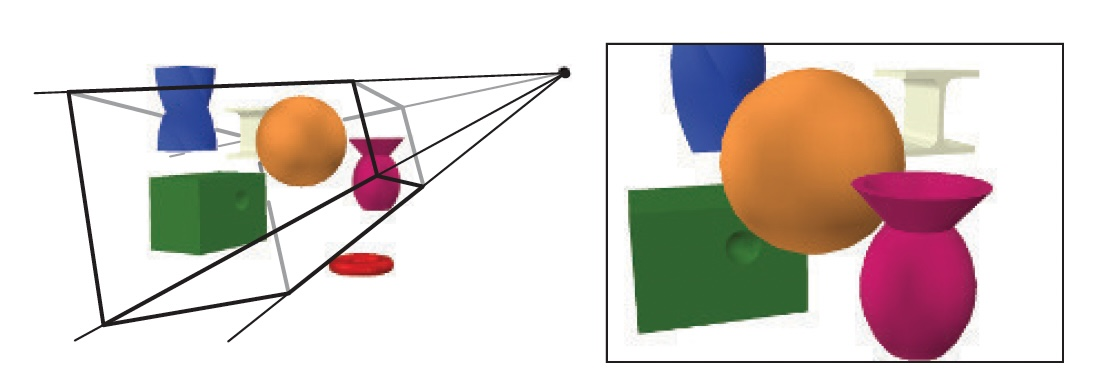
\includegraphics[width=\textwidth]{img/Render/render_pipeline_1.jpg}
    \caption{Die dreidimensionale Szene (links) und die zweidimensionale Sicht der virtuellen Kamera. Wird das Objekt perspektivisch gerendert, gibt es ein Raumvolumen (frustum). Es werden nur die Objekte gerendert, die sich innerhalb dieses Volumens befinden. So wird der rote Donut nicht und das blaue Objekt abgeschnitten dargestellt\cite*[Moeller (2019)]{moeller2019}.}
    \label{fig:renderpipeline1}
\end{figure}

Die \acrshort{grafik-rendering-pipeline} wird in vier Hauptstufen unterteilt: 

\begin{itemize}
    \item Applikation,
    \item Geometrieverarbeitung,
    \item Rasterisierung,
    \item Pixelverarbeitung.
  \end{itemize}

\begin{figure}[H]
    \centering
    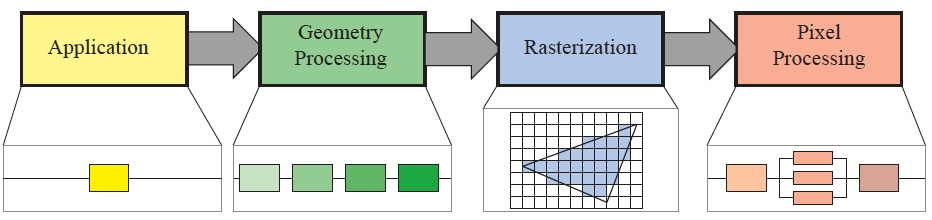
\includegraphics[width=\textwidth]{img/Render/render_pipeline_2.jpg}
    \caption{Die Basis der \acrshort{grafik-rendering-pipeline}, die in weitere Sub-Pipelines eingeteilt und parallel ausgeführt werden können \cite*{moeller2019}.}
    \label{fig:renderpipeline2}
\end{figure}

Die Abarbeitung der Aufgaben in den verschiedenen Stufen wird parallel ausgeführt. Durch die Parallelisierung ist eine verbesserte Performance möglich, da nicht jeder Prozess Schritt für Schritt durchgeführt werden muss. Jede Stufe kann gleichzeitig eine weitere Sub-Pipeline benutzen. So hat die Stufe \textit{Geometrieverarbeitung} in der Abbildung \ref*{fig:renderpipeline2} die Aufgabe in eine Sub-Pipeline gegliedert, die wiederum parallel ausgeführt werden kann. Die render Geschwindigkeit wird in \textit{frames pro sekunde} (\acrshort{frames-per-second}) angegeben und repräsentiert die Anzahl an Bilder, die pro Sekunde gerendert werden\cite*[Moeller (2019)]{moeller2019}. 

\subsubsection{Applikationsstufe}
Die Hauptaufgabe der Appliaktionsstufe besteht darin die benötigten Daten in die Pipeline zu schicken und zu aktualisieren. Die Daten bestehen aus den Render-Primitiven, die beispielsweise Punkte, Linien, Dreiecke oder Polygone (Vielecke) darstellen. Am Ende der Applikationsstufe werden die Rendering-Primitive an die Geometrieverarbeitungsstufe weitergegeben. Weiterhin finden Interaktionen wie z.B. Kollisionsabfragen statt oder es werden Input-Daten von Maus und Tastaur verarbeitet. Auch werden Culling-Algorithmen\footnote{ein Algorithmus, bei dem bestimmte (z.B. verdeckte) Polygone nicht gerendert werden, um eine bessere Performance zu erzielen \cite*{coorg1997}.} ausgeführt. Die Applikationsstufe wird im Gegensatz zu den anderen Stufen meist auf der \acrshort{cpu} ausgeführt. Entwickler haben dadurch eine hohe Kontrolle über die Prozesse in dieser Stufe. Sie können die Implementierung selbst bestimmen und im nachhinein modifizieren, um z.B. die Performance weiter zu verbessern\cite*[Moeller (2019)]{moeller2019}.

\subsubsection{Geometrieverarbeitung}
Auf dieser Stufe finden Operationen an den Polygonen und Vertices (Eckpunkte) statt. Sie wird auf der \acrshort{gpu} ausgeführt und lässt sich in eine Sub-Pipeline in Vertex-Shading, Projektion, Clipping und Window-Viewport-Transformation unterteilen.

\subsubsubsection{Vertex-Shading}
\label{grp-geometrieverarbeitung-vertex-shading}
Ein Vertex-Shader ist ein programmierbarer Shader in der Rendering-Pipeline, der die Eigenschaften jedes einzelnen Vertex bestimmt. Ein Vertex beinhaltet die Koordinaten von Punkten im dreidimensionalen Raum. Mithilfe von Informationen, welche Vertices miteinander verbunden sind, werden Linien und Polygone definiert \cite*[Vgl. Nischwitz (2012) S.48.]{nischwitz2012}. Die Aufgabe des Vertex-Shaders ist es, die Modellkoordinaten der Vertices durch Translation, Rotation oder Skalierung zu transformieren, um die Modelle zunächst im Weltkoordinatensystem, dann im Kamerakoordinatensystem und zuletzt im Clipping-Koordinatensystem zu lokalisieren. Die Transformationen werden mit 4x4 Transformtionsmatrizen durchgeführt. Der Vertex-Shader berechnet die Position eines Vertex von seinem Modellkoordinatensystem zum Clipping-Koordinatensystem:

\begin{equation}
    p'=P*K*W*p
    \label{vertex-transformationen}
\end{equation}
wobei:
\begin{conditions*}
    p'  &   Vertex in Clip-Koordinaten\\
    P   &   Projektionsmatrix \\
    K   &   Kamera-Transformation \\
    W   &   Welt-Transformation\\
    p   &   Vertex in Modellkoordinaten
\end{conditions*}

Die Reihenfolge der Transformationen spielt eine wichtige Rolle, da die Matrizenmultiplikation nicht kommutativ ist. Die Transformationen in der Gleichung \ref*{vertex-transformationen} müssen daher von rechts nach links durchgeführt werden.

Die Vertices der Modelle befinden sich ursprünglich in ihrem eigenen Modellkoordinatensystem. Die Szene hat ein Weltkoordinatensystem und ein Kamerakoordinatensystem. Die Vertices werden zunächst in das Weltkoordinatensystem transformiert. Die Kamera in der Szene hat Koordinaten im Weltkoordinatensystem und eine Richtung, in die die Kamera zeigt. Mit der Kamera-Transformation werden die Vertices und die Kamera so platziert, dass die Kamera in der Position des Ursprungs des Weltkoordinatensystems liegt und (meist) in negativer z-Richtung zeigt, während die y-Achse nach oben und die x-Achse nach rechts zeigt. Die genaue Definition der Richtungen der Koordinatenachsen hängt von der jeweiligen Anwendung ab. Das daraus folgende Koordinatensystem wird Kamerakoordinatensystem genannt. Somit befinden sich die Vertices nach den Kamera-Transformationen im Kamerakoordinatensystem. Schließlich wird eine Projektionsmatrix angewandt, um die Kamerakoordinaten der Vertices in Clipping-Koordinaten zu transformieren.

Zusätzlich zu den Transformationen bestimmt ein Vertex-Shader Eigenschaften wie die Farbe, Texturkoordinaten oder Normalenvektoren für jeden Vertex. Diese beschreiben das Material des Objekts und Effekte von Lichtquellen, die auf die Oberfläche scheinen. Die Wirkung von Licht auf ein Material wird Shading genannt. Es werden "[..]Normalenvektoren und Materialeigenschaften der Objekte auf der einen Seite und den Eigenschaften der Lichtquellen auf der anderen Seite für jeden Vertex die Beleuchtungsrechnung durchgeführt und somit eine Farbe ermittelt" \cite*[Nischwitz (2012) S.48,][]{nischwitz2012}. Die Ergebnisse der Berechnungen werden zur Rasterisierung und zur Pixelverarbeitung weitergeschickt\cite*[Moeller (2019)]{moeller2019}.

Mit Vertex-Shadern ist es möglich Oberflächen realistisch darzustellen, ohne die Polygonanzahl zu erhöhen. So nutzen Mitchell\cite*[][]{mitchell2005} und Isidoro \cite*[][]{isidoro2002} Vertex-Shader, um mit Heightmaps %Link und Kapitel Heightmaps
und Normalmaps %Link und Kapitel Normalmaps
einen realistischen Ozean zu rendern.

\subsubsubsection{Projektion}
\label{grp-geometrieverarbeitung-projektion}
Bei der Projektion werden zwei Aufgaben durchgeführt. Zum einen wird ein Clipspace (Kanonisches-Sichtvolumen) definiert, das meist in Form eines Einheitswürfels\footnote{ein Würfel mit der Skalierung (1,1,1)} gegeben ist. Der Würfel ist für das Clipping von Bedeutung.

Zum anderen wird eine Projektionsmethodik je nach Anwendungsfall bestimmt. Beispielsweise gibt es eine orthographische Projektion, bei der parallele Linien auch parallel erscheinen, während bei der perspektivischen Projektion parallele Linien Fluchtpunkten folgen. Die Projektionsmethodik bestimmt die Projektionsmatrix für die Transformation in die Clipping-Koordinaten.

\subsubsubsection{Clipping}
\label{grp-geometrieverarbeitung-clipping}
Nur mit den im Vertex-Shader transformierten Clipping-Koordinaten der Vertices kann Clipping durchgeführt werden. Es werden nur die Primitiven zur Window-Viewport-Transformation weitergeschickt, die sich innerhalb des kanonischen-Sichtvolumens befinden. Clipping wird dann benötigt, wenn sich ein Teil eines Primitiven innerhalb und ein anderer Teil außerhalb des Sichtvolumens befinden. Die Primitiven, die sich mit dem Einheitswürfel schneiden, erhalten an der Schnittkante neue Vertices\cite*[Moeller (2019)][]{moeller2019}.

\subsubsubsection{Window-Viewport-Transformation}
\label{grp-geometrieverarbeitung-window-viewport-transformation}
Im nächsten Schritt wird mit den Primitiven eine Window-Viewport-Transformation durchgeführt. Dadurch wird es möglich die x- und y-Koordinaten der Primitiven auf ein Bildschirmausschnitt (Viewport) darzustellen. Die Primitiven erhalten Bildschirm- bzw. Window-Koordinaten\footnote{Bildschirm-Koordinaten sind zweidimensionale (x,y)-Koordinaten, während Window-Koordinaten auch die z-Koordinate beinhaltet (x,y,z).}. Es handelt sich dabei um eine Translation gefolgt von einer Skalierung\cite*[Moeller (2019) S.20f.,][]{moeller2019} \cite*[Nischwitz (2012) S.150,][]{nischwitz2012}.

\subsubsection{Rasterisierung}
\label{grp-rasterisierung}
Bei der Rasterisierung werden mit einer perspektivischen Projektion Pixel gesucht, die sich auf dem Viewport innerhalb der gerenderten Primitiven befinden. Es findet eine Übersetzung der 3D-Koordinaten in 2D-Pixelkoordinaten statt. Klassische Rasterisierungs-Algorithmen definieren einen zugehörigen Pixel genau dann, wenn ein Pixel sich innerhalb eines Primitiven befindet. Es werden sogenannte \textit{Fragmente} für den Teil des Pixels erzeugt, der sich mit dem Dreieck überschneidet\cite*[][, zuletzt aufgerufen am 11.07.2022]{scratchapixel} cite*[Moeller (2019) S.21f.,][]{moeller2019}. 

\begin{figure}[hbt!]
    \centering
    \subfloat[][]{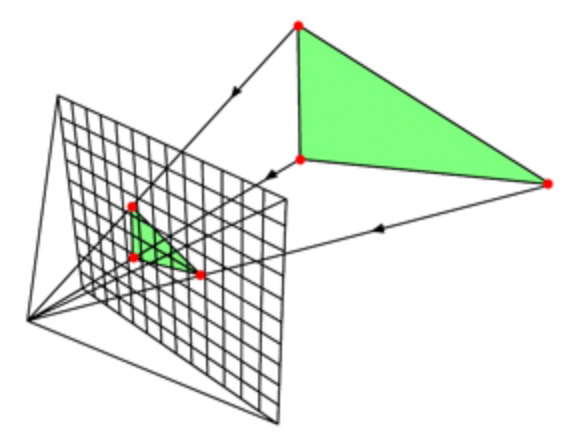
\includegraphics[width=0.4\linewidth]{img/Render/rasterisierung_1.jpg}}%
    \qquad
    \subfloat[][]{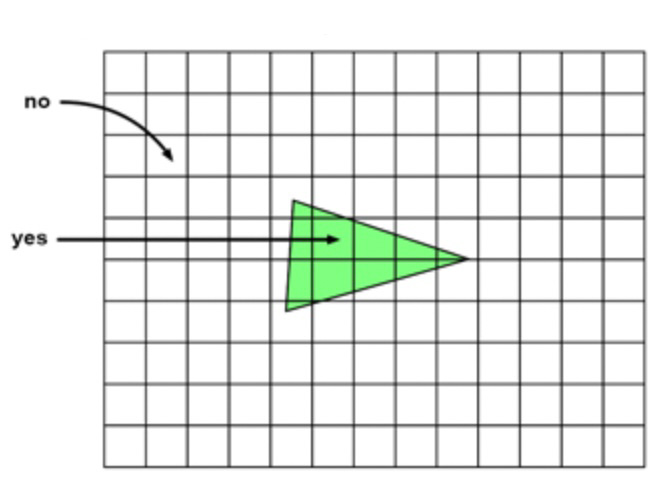
\includegraphics[width=0.4\linewidth]{img/Render/rasterisierung_2.jpg}}%
    \caption{Die Primitiven werden in eine 2D-Ebene projiziert(a). Befindet sich ein Pixel innerhalb des Primitiven, werden diskrete Fragmente gebildet, die im in der Pixelverarbeitung weitergeschickt werden(b) \cite*[][, zuletzt aufgerufen am 11.07.2022]{scratchapixel}.}%
    \label{fig:rendering-pipeline-rasterisierung-beispiel}
\end{figure}

\subsubsection{Pixelverarbeitung (Fragment-Shader)}
\label{grp-pixelverarbeitung}
Bei der Pixelverarbeitung werden die diskreten Fragmente aus der Rasterisierung mit einem Fragment-Shader verarbeitet. So werden im einfachsten Fall die endgültigen Farben der Fragmente festgelegt oder auch Texturen an das Modell angeheftet. 
%Eigenes Beispiel mit gescheiten Outline Shader zeigen!

Nach dem Fragment-Shader wird überprüft, ob sich im dreidimensionalen Raum zwei oder mehrere Fragmente überlappen. Für diesen Fall gibt es einen z-Buffer, der für jedes Fragment einen z-Wert gespeichert hat. Dieser z-Wert repräsentiert wie weit das Fragment von der Kamera entfernt ist. Ein z-Buffer Algorithmus entscheidet dann, welches Fragment näher zur Kamera liegt und welche Farbe das Fragment letzendlich haben soll. Dieser Algorithmus ist simpel und hat den Vorteil, dass die render Reihenfolge der Primitiven trivial ist. Probleme gibt es jedoch bei transparenten Objekten. Hier ist die Reihenfolge für eine korrekte Darstellung wichtig\cite*[Moeller (2019) S.21f.,][]{moeller2019}. Für eine ausführliche Erklärung für den Umgang mit transparenten Objekten wird auf Möller, Kapitel 5.5 verwiesen\cite*[Moeller (2019) S.148ff.,][]{moeller2019}.
% -- Schatten

% Ähnliche Arbeiten
%\section{Forschungsstand}
Augmented Reality ist ein nachgefragtes Thema und wird in unterschiedlichen Bereichen wie Industrie, Medizin oder in der Computerspiel-Branche untersucht\cite{Sudirman}\cite{Santi}\cite{Huang}. Es gilt Probleme zu lösen, die sowohl Hardware als auch Software betreffen. Die Hardwareentwicklung betrifft dabei hauptsächlich die Mobilität bei der Nutzung. Beispielsweise funktioniert die HTC Vive nur mit einem Computer, der mit einem Kabel am Headset verbunden ist. Die Microsoft Holo Lens hingegen benötigt eine gute Internetverbindung über Wi-Fi. In der Software ist es eine Herausforderung aus den vielfältigen Software-Paketen eigene AR Anwendungen zu entwickeln. Nicht jede Software Bibliothek ist miteinander kompatibel, sodass die Entwicklung eine lange Einarbeitungszeit benötigt\cite*[Vgl.][]{Santi}.

Ein weiteres Problem in der Nutzung von AR ist die Beleuchtung der Umgebung. In Fabriken oder Lagern ist es dunkel und Lichter kommen aus verschiedenen Richtungen, während es im Freien die Wetterbedingungen wie starke Sonne oder Wolken, die störende Schatten verursachen, zu beachten gilt. Die unterschiedlichen Lichtverhältnisse rufen Ungenauigkeiten z.B. beim Tracking hervor.

\subsection{Tracking}
Der Begriff Tracking beschreibt die kontinuierliche Verfolgung von Positions- und Rotationsdaten, die von Eingabegeräten (z.B. VR Controller) oder Sensoren (z.B. \textit{Inertial Measurement Units} (Gyroskop und Beschleunigungssensoren)) erfasst werden. Die Bewegung eines starren Körpers kann \glqq durch die Angabe von sechs Werten (drei Koordinaten als Position und drei Winkel zur Beschreibung der Orientierung) für jeden Zeitschritt spezifiziert werden\grqq{}\cite*[Dörner (2019) S.119f.]{doerner}. 

Die Werte für die Position und Orientierung für ein Objekt werden als \textit{Freiheitsgrade (engl. Degrees of Freedom – DOF)} bezeichnet. Beim Tracking ist es das Ziel, die sechs Freiheitsgrade
für die Translation und Rotation der Kamera zu bestimmen bzw. zu schätzen\cite{doerner}. Es gibt zwei Tracking Systeme. Beim \textit{Inside-Out-Tracking} befinden sich Sensoren im Objekt, das getrackt werden soll, während beim \textit{Outside-In-Tracking} sich die Sensorik in der Umgebung befinden und das Objekt von außen getrackt wird. In dieser Arbeit wird ein Inside-Out-Tracking verwendet, da sich die Sensorik im Smartphone bzw. Tablet befinden.

\subsubsection{Koordinatensysteme}
Um eine Bestimmung bzw. Schätzung der Translationen und Rotationen durchzuführen, können zwei Koordinatensysteme herangezogen werden. Ein Kamerakoordinatensystem und ein Objektkoordinatensystem, womit die relativen Transformationen zwischen den Koordinatensystemen bestimmt werden können. Weiterhin gibt es die Möglichkeit, dass für alle Objekte im Raum ein Koordinatensystem (Weltkoordinatensystem) verwendet wird. Voraussetzung für das Tracking ist, dass die Transformationen zwischen den Objekten bekannt sind. Dann kann die Transformation zwischen der Kamera und das Weltkoordinatensystem geschätzt werden. Sind einzelne Transformationen von Objekten im Weltkoordinatensystem nicht bekannt, kann es auch Mischformen geben Zitat \cite*[Dörner (2019) S.124f.]{doerner}.

\subsection{Kamera-basiertes Tracking}
Kamera-basiertes Tracking nutzt Informationen zu Objekten aus dem Video Datenstrom, um die relative Position und Orientierung der Objekte zur Kamera zu bestimmen. Hartley und Zisserman bezeichnen diese als \textit(extrinsische Kameraparameter) \cite*[Hartley, Zisserman (2003) S.156]{hartleyzisserman}. Für das Kamera-basierte Tracking wird zwischen Marker-basierten und Marker-less Tracking unterschieden.

Beim Marker-basierten Tracking werden schwarz-weiß Marker (sogenannte Kanji und Hiro Marker) (Verweis) mit einfachen geometrischen Formen platziert und erkannt, sodass diese als als Orientierungshilfen fungieren. Eine Anwendung von NGIN-Mobility arbeitet mit Markern, die auf dem Boden platziert werden können \footnote{https://www.logistik-watchblog.de/startups/1479-insider-navigation-ar-loesung-lagerhalle.html}. Da die Marker in dauerhaft in der Umgebung platziert werden müssen, ist die Trackingmöglichkeit für die Nutzung im Freien ungeeignet.

Die zweite Möglichkeit erfasst über Algorithmen der Computer Vision Merkmale in der realen Umgebung. Diese Art wird als \textit{marker-less AR} bezeichnet. Merkmale können geometribasiert sein (z.B. Kanten, Formen wie Vierecke) oder es werden Detektoren wie z.B. \textit{SIFT (engl. Scale Invariant Feature Transform)}\cite{lowe1999} oder \textit{SURF (engl. Scale Invariant Feature Transform)}\cite{bay2008} verwendet. Auch die aus der Robotertechnik bekannte \textit{SLAM (engl. Simultaneous Localization and Mapping)}\cite{slam1} \cite{slam2} Methode wird genutzt. Dabei werden entweder kamerabasiert (Visual SLAM) nach Merkmalen gesucht oder es kommen Sensoren zur Generierung von Tiefeninformationen zum Einsatz, z.B. Kinect \footnote{https://developer.microsoft.com/de-de/windows/kinect/} oder \textit{LIDAR-Sensoren (engl. light detection and ranging)}\cite{Liu2020}. Vorteil dieser Methode ist, dass gleichzeitig eine 3D-Karte des Raumes generiert wird, die immer wieder zur Positions- und Rotationsbestimmung verwendet werden kann.

\subsubsection{GPS Tracking}
Im Außenbereich wird bei AR auch GPS für das Tracking herangezogen. Dabei sind Positionsabweichungen von bis zu 10 Metern möglich, sodass eine genaue Bestimmung der extrinsischen Kameraparameter beeinträchtigt wird. Um die Tracking-Genauigkeit zu erhöhen, gibt es mehrere Methoden. \textit{DGPS (engl. Differential GPS)} verbessert GPS-Signale, indem es ein Korrektursignal durch eine ortsfeste Referenzstation mit bekannter Lokalisierung berechnet. Da es in Deutschland lediglich acht solcher Stationen gibt und einige Anbieter nur kommerziell die Daten bereitstellen, ist diese Methode nicht für diese Arbeit geeignet\footnote{https://www.heise.de/newsticker/meldung/Differential-GPS-und-WLAN-RTT-Praezise-Ortung-mit-Android-P-4046935.html} \footnote{Liste von DGPS-Sendern: https://www.ndblist.info/datamodes/worldDGPSdatabase.pdf}. Eine weitere bekannte Möglichkeit bietet \textit{SBAS (engl. Satellite Based Augmentation System)}, bei dem mehrere geostationäre Satelliten das GPS Signal auf bis zu einem Meter Genauigkeit zu verbessern \cite*{doerner}.

Platinsky und seine Koautoren\cite{platinsky} erstellen für ein besseres Tracking bei fehlender GPS Genauigkeit ein 3D-Modell der Umgebung. Bei der anschließenden AR Nutzung in diesem Gebiet wird auf dem Smartphone SLAM betrieben. Die Daten vom Smartphone werden mit der 3D-Karte verglichen, um ein genaueres Tracking durchzuführen. Ein ähnliches System wäre für die Anwendung in dieser Arbeit denkbar, da eine große Datenmenge von Bildern des Geländes vorhanden ist. Über Structure from Motion Methoden, kann mit den Bildern eine große 3D-Karte erstellt werden.

\begin{figure}[h]
    \centering
    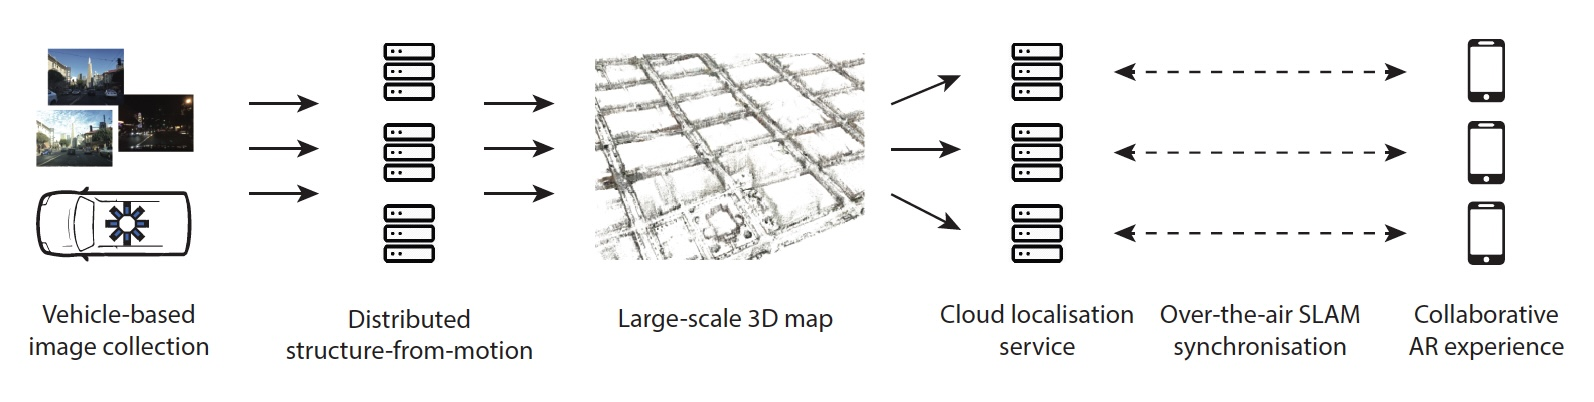
\includegraphics[width=\textwidth]{platinsky.jpg}
    \caption{Das Grundprinzip der Methode von Platinsky.}
    \label{fig:PlatinskyPrinzip}
\end{figure}

\subsection{Software Entwicklung}
Für Augmented Reality Anwendungen gibt es im Smartphone und Tablet Bereich mehrere Softwarepakete (\textit{SDK (engl. Software Development Kit)}. Die bekanntesten sind ARKit von Apple, das nur auf iOS Endgeräten läuft und ARCore von Google, das für Android Endgeräte entwickelt wird.\footnote{https://developer.apple.com/augmented-reality/} \footnote{https://developers.google.com/ar} Andere SDK's wie Vuforia\footnote{https://www.ptc.com/en/products/vuforia}, Wikitude\footnote{https://www.wikitude.com/}, ARToolKit\footnote{http://www.hitl.washington.edu/artoolkit/} oder Lightship\footnote{https://lightship.dev/} sind unabhängig vom Endgerät nutzbar.  

\section{Fragestellungen und Methodik}
Für die Entwicklung der AR Anwendung können die vorgestellten SDK's genutzt werden. Diese haben Vor- und Nachteile, die in dieser Arbeit erörtert werden, um daraus die passende SDK für dieses Projekt auszuwählen. Die Methode von Platinsky und seinen Koautoren\cite{platinsky}, in der das Tracking durch eine vorgefertigte 3D-Karte der Stadt verbessert wird, wird in dieser Arbeit weiter untersucht. Im Beispiel von Platinsky ist die GPS Genauigkeit durch die hohen Gebäude in der Großstadt stark beeinträchtigt. Das Gelände in Villingen befindet sich am Stadtrand und die Gebäude könnten keinen großen Einfluss auf die GPS Genauigkeit haben. Daher wird untersucht, ob der Mehraufwand, der durch die Erstellung der 3D Map und des SLAM Systems über eine Cloud entsteht, für eine mittelgroße Stadt sinnvoll ist. Hierfür wird die GPS Genauigkeit mit und ohne dieser Methode gemessen und miteinander verglichen.

Hinzu kommt die Frage, wie detailreich die 3D-Karte und die SLAM Daten des Smartphones für ein genaues Tracking sein müssen. Ein Problem der Methode ist, dass eine konstante Verbindung zum Internet bestehen muss, um die SLAM Daten mit der 3D-Karte zu vergleichen. Die 4G Verbindung war nicht ausreichend schnell \cite*[][sinngemäß aus]{platinsky}. Um an diesem Problem anzuknüpfen, wird untersucht, wie stark die Qualität der 3D-Karte reduziert werden kann, ohne die Vorteile beim Tracking zu verlieren. Eine Optimierung der Dateigröße der 3D-Karte wird im Paper zwar erwähnt, jedoch nicht umgesetzt. So wird in dieser Arbeit ein Experiment durchgeführt, bei der drei Qualitätsstufen (Hohe Details, mittlere Details, grobe Details) auf die GPS Genauigkeit untersucht werden. 

Je nachdem wie die Ergebnisse der Experimente ausgehen, ist es für die Anwendung sinnvoll dem Nutzer zwei Möglichkeiten anzubieten: Eine hohe Tracking Genauigkeit bei hohem Datenverbrauch und eine möglicherweise geringe Tracking Genauigkeit, bei dem diese Methode nicht genutzt wird.


%KAPITEL 3 Konzept
% Konzept
\section{Konzeption der Anwendung}
In diesem Abschnitt wird das Konzept vorgestellt. Es werden die Interaktionsmöglichkeiten des Nutzers erläutert und ein grober Ablauf der Anwendung aufgezeigt. Mithilfe eines Use-Case-Diagramms wird der Ablauf grafisch dargestellt. Ein Use-Case Diagramm ist ein Verhaltensdiagram der \textit{\acrfull{uml}}. Es repräsentiert grafisch Anwendungsfälle für eine Software und beinhaltet eine Beschreibung der Funktionen, der Akteure und deren Beziehungen in einem System\footnote{https://de.wikipedia.org/wiki/Anwendungsfalldiagramm, zuletzt aufgerufen am 10.08.2022}. Das Kapitel \ref*{} geht dann auf die technische Umsetzung ein.

\subsection{Idee und Ablauf}
\label{konzept-der-anwendung}
Das Ziel der Anwendung ist es dem Nutzer die historischen Gebäude sowohl vor Ort als auch an einem beliebigen Ort zu zeigen. Die Gebäude werden so dargestellt, dass sie sich nahtlos in das reale Bild einfügen. Dafür wird auf die richtige Belichtung und auf korrekte Schattenwürfe geachtet. 

Je nach Tageszeit verändert sich die Farbtemperatur des Lichts. Zum Sonnenaufgang und zum Sonnenuntergang färbt sich z.B. das Hauptlicht rötlich, während im Tageslicht die Farbtemperatur neutral ist. Ist es Nacht, scheint kein Licht auf die Gebäude. Zusätzlich wird das Gebäude den herrschenden Wetterbedingungen angepasst. 

Eine Anbindung zur Wetter \acrfull{rest} API \textit{Open-Weather-Map}\footnote{https://openweathermap.org/, zuletzt aufgerufen am 10.08.2022} fragt das aktuelle Wetter am Ort des Nutzers ab. 

Eine REST API ermöglicht den Austausch von Informationen von unterschiedlichen Systemen. Die Informationen, die in diesem Fall die Wetterdaten sind, liegen auf Servern, die mit Hilfe eines HTTP-Requests angefordert werden\footnote{https://www.codecademy.com/article/what-is-rest, zuletzt aufgerufen am 19.08.2022}. Mit der Antwort der API werden dann Parameter für das Licht wie in Kapitel \ref*{technische-umsetzung-licht} und des verwendeten Fragment-Shaders verändert. Die genaue technische Umsetzung wird in Kapitel \ref*{technische-umsetzung-wetterbedingungen} behandelt. 

Das Use-Case Diagramm in Abbildung \ref*{fig:konzept-use-case-diagramm} zeigt den Ablauf der Anwendung.

\begin{figure}[H]
    \centering
    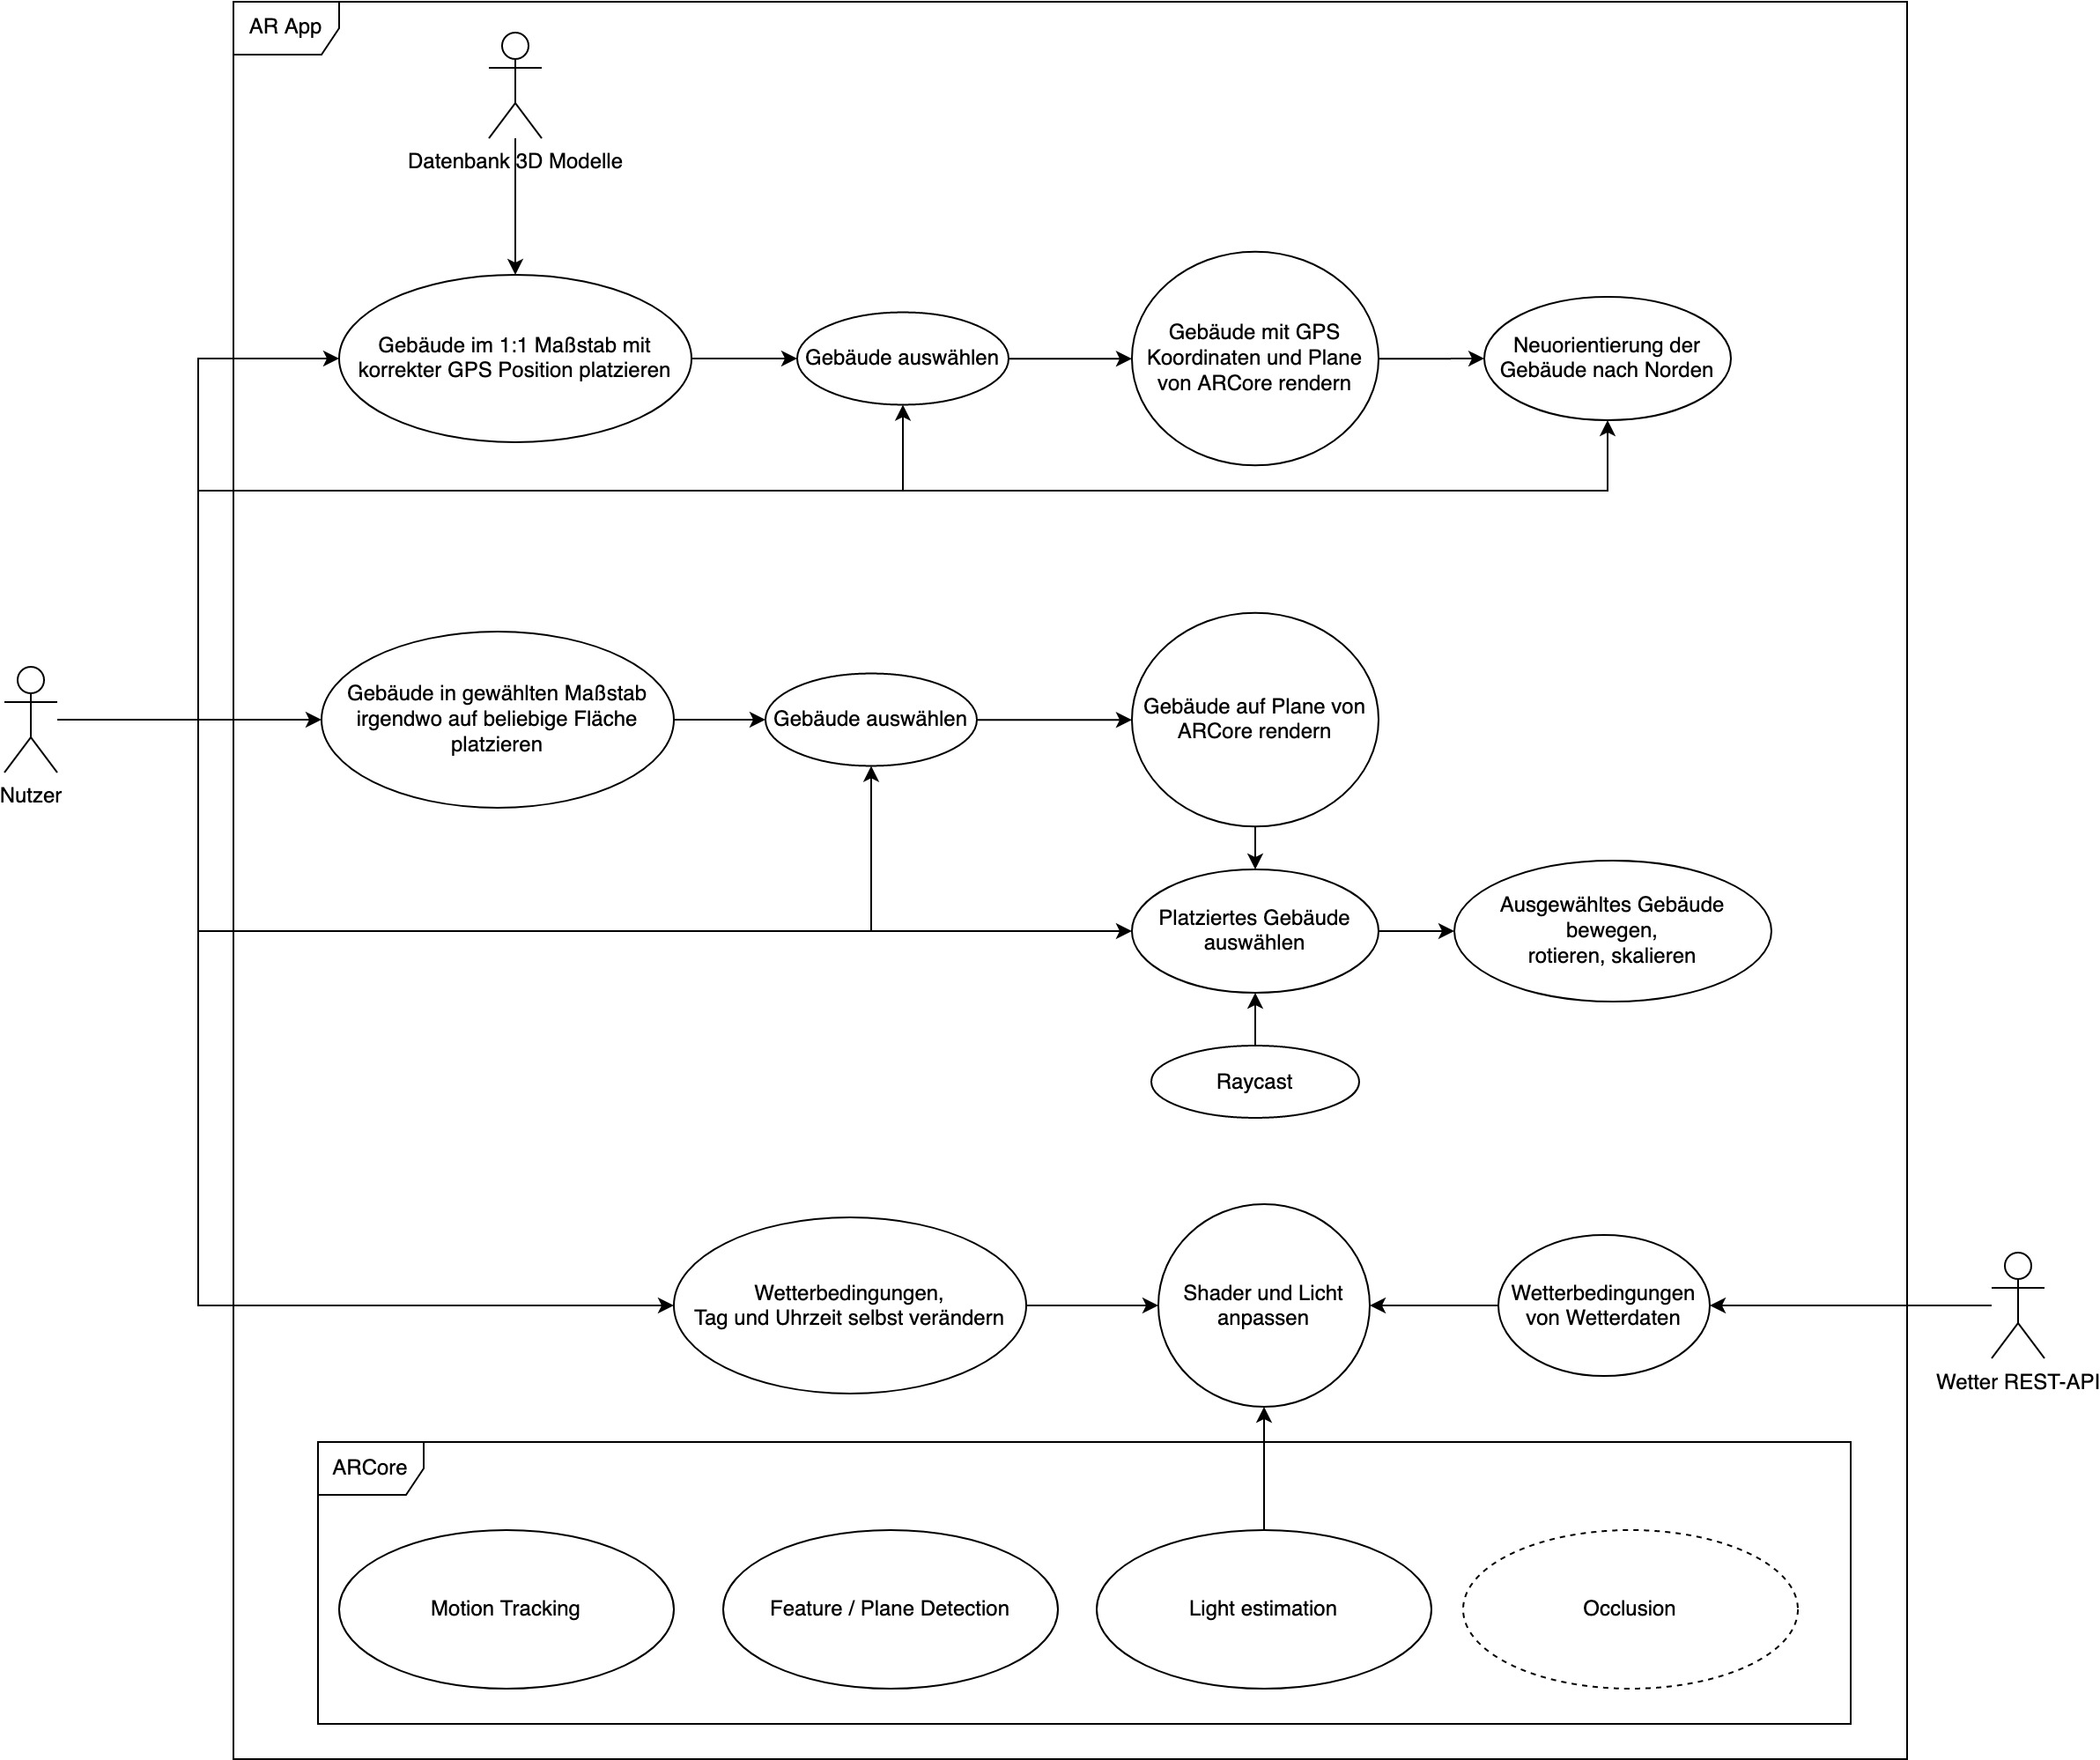
\includegraphics[width=\textwidth]{img/anwendung/UseCaseDiagrammVillingenAR.jpg}
    \caption[Das Use-Case-Diagramm zur Anwendug.]{Das Use-Case-Diagramm zur Anwendug.\protect\footnotemark}
    \label{fig:konzept-use-case-diagramm}
\end{figure}
\footnotetext{Quelle Bild: https://drive.google.com/file/d/1ZhIIEN6V9Jt-uwVcFVNkeFbu1qxbGkaN/view?usp=sharing}

In der Anwendung gibt es drei Akteure: Der Nutzer, die REST-API für die Wetter-Abfrage und eine interne Datenbank mit den Daten zu den Gebäuden. Die interne Datenbank enthält die Informationen zu den Gebäuden, die für die Anwendung benötigt werden. Die Informationen sind:
\begin{itemize}
    \item die 3D Modelle als \textit{Prefab}. Ein Prefab ist ein GameObject in Unity, dass alle Komponenten, Werte und angehängte GameObjects beinhaltet. Sie erlauben dieses GameObject zu speichern und mit den gleichen Informationen wieder zu verwenden\footnote{https://docs.unity3d.com/Manual/Prefabs.html, zuletzt aufgerufen am 13.08.2022},
    \item der Name des Gebäudes, wie z.B. das SABA Hauptgebäude oder das Mannschaftsgebäude,
    \item eine Kurzbeschreibung. Diese wird noch nicht genutzt. Die Idee dazu ist, zusätzlich zum 3D Modell noch eine Kurzbeschreibung des Gebäudes und dessen ehemalige Funktion in AR einzublenden,
    \item die Längen- und Breitengrade für die GPS-Platzierung,
    \item eine Winkelangabe. Diese wird benötigt, um bei einer Ausrichtung nach Norden die Gebäude mit der korrekten Rotation darzustellen,
    \item eine ID-Nummer zur Identifizierung.
\end{itemize}

Die Datenbank wird in Unity mit \texttt{ScriptableObjects}\footnote{https://docs.unity3d.com/Manual/class-ScriptableObject.html, zuletzt aufgerufen am 13.08.2022} realisiert. Das ist ein Datencontainer, indem individuelle Daten gespeichert werden können. Für jedes Objekt wird ein \texttt{BuildingGPS} Scriptable Object erzeugt, indem die jeweiligen Daten gespeichert sind. Die Nutzung der Daten wird in Kapitel \ref*{technische-umsetzung-platzierung-normal} und \ref*{technische-umsetzung-platzierung-gps} behandelt.

Zu Beginn der Anwendung kann der Nutzer in einem Menü sich zwischen zwei Möglichkeiten der Platzierung entscheiden:
\begin{itemize}
    \item das Gebäude wird über GPS Koordinaten platziert,
    \item das Gebäude wird auf einer von ARCore getrackten Flächen platziert.
\end{itemize}

Anschließend wird die jeweilige AR Szene gestartet. An diesem Zeitpunkt wird ARCore gestartet. Die Funktionen wie z.B. das Motion Tracking oder die Plane Detection aktivieren sich. Der Nutzer wählt daraufhin das Gebäude aus, das platziert werden soll. Eine Vorschau des Modells und der Name des Gebäudes werden angezeigt. Dieses Menü ist in Abbildung \ref*{fig:konzept-auswahl-menue} zu sehen. 

\begin{figure}[H]
    \centering
    \subfloat[][]{\includegraphics[width=0.3\linewidth]{img/anwendung/konzept-auswahl-menü.jpg}}%
    \qquad
    \subfloat[][]{\includegraphics[width=0.3\linewidth]{img/anwendung/konzept-auswahl-menü-2.jpg}}%
    \caption{Das Auswahl-Menü. Der Nutzer kann mit dem Burger-Icon das Menü jederzeit öffnen und wieder schließen. Mit den Pfeilen kann zwischen den vorhandenen Gebäuden geschaltet werden.}%
    \label{fig:konzept-auswahl-menue}
\end{figure}

Ist ein Gebäude ausgewählt, ist die Platzierung des Gebäudes möglich. Voraussetzung ist, dass ARCore eine Fläche gefunden hat. Sobald eine Fläche vorhanden ist, wird über Raycast ein Hit-Testing durchgeführt (siehe Kapitel \ref*{technische-umsetzung-arcore-user-interaction}). Ist ein Hit regisitriert, ist eine Fläche für die Platzierung vorhanden. Der Nutzer erhält Feedback über ein Pfeil-Icon, das auf die jeweilige Fläche platziert wird. Dieser hilft dem Nutzer bei der Orientierung und der Platzierung der Objekte.

\subsection{Platzierung auf einer beliebigen Fläche}
Der Pfeil auf dem Boden zeigt an, wo die Position des Gebäude sein wird. Nach der Auswahl des Modells kann der Nutzer über ein Tap auf dem Bildschirm das Gebäude platzieren. Über einen Raycast wird das platzierte Modell erkannt und der Nutzer kann mit einem Button das platzierte Gebäude auswählen. Dieses kann per Drag Gesten über erkannte Flächen verschoben werden. Mit einer Pinch Geste wird das Gebäude skaliert. Über einen Slider wird die Rotation verändert. Nur ausgewählte Gebäude können bewegt, skaliert, rotiert und gelöscht werden. Es ist nur möglich eine Instanz von einem Gebäude zu platzieren.

\subsection{Platzierung über GPS}
Bei der GPS Platzierung wird die aktuelle GPS Position abgefragt. Mit den Längen- und Breitengraden aus der Datenbank werden die Gebäude bezüglich der GPS Position des Smartphones platziert. Damit das Gebäude nicht in der Luft schwebt, wird es auf eine Fläche platziert, die ARCore detektiert hat. Der Nutzer hat hier nicht die Möglichkeit ein Gebäude auszuwählen, da diese Funktion nur vor Ort funktioniert. Der Sinn dieser Funktion ist es, dem Nutzer die Gebäude so zu zeigen, wie sie vor Ort ausgesehen haben. Die Gebäude werden an der jeweiligen Position im Größenverhältnis 1:1 dargestellt.

Der Nutzer hat zusätzlich die Möglichkeit mithilfe des Kompass des Gerätes die Szene nach Norden auszurichten. Damit wird sichergestellt, dass das Gebäude in der korrekten Rotation dargestellt wird. In der Datenbank ist das 3D Modell zusammen mit einer Winkelangabe gespeichert. Diese wird benötigt, um das Gebäude so zu drehen, dass es in die korrekte Richtung zeigt. Die technische Umsetzung wird in Kapitel \ref*{technische-umsetzung-platzierung-gps} behandelt.

\subsection{Licht und Wetterbedingungen ändern}
Die Wetterbedingungen werden beim Start der Anwendung von der REST-API abgefragt. Hierfür wird eine Internetverbindung benötigt. Die Informationen zu Wetter und Tageszeit werden dazu, genutzt das Licht und die Shader der Gebäude anzupassen. Zusätzlich wird die Light estimation Funktion von ARCore genutzt, um die Farbtemperatur und die Helligkeit anzupassen.

%KAPITEL 4 Umsetzung
% Vorbereitung Blender Modelle
\section{Vorbereitung der 3D Modelle in Blender}
Einige 3D Modelle haben durch die umliegende Vegetation unvollständige oder mit der Vegetation verschmolzene Meshes. In der Projektarbeit des Wintersemesters 2020/21 wird das Problem näher beschrieben \cite*{kusch2021}.

\subsection{Lückenhafte Wände füllen}
Das Gebäude 2 des Lyautey Geländes hat eine Haushälfte, die mit einem Baum verschmolzen ist und es fehlt daher ein Teil der Wand. Da das Gebäude symmetrisch und die gespiegelte Seite fehlerfrei ist, wird ein Teil dieser Wand als Lückenfüller eingesetzt. Im folgenden wird die Nachbearbeitung an diesem Modell beschrieben.

\begin{figure}[ht]
    \centering
    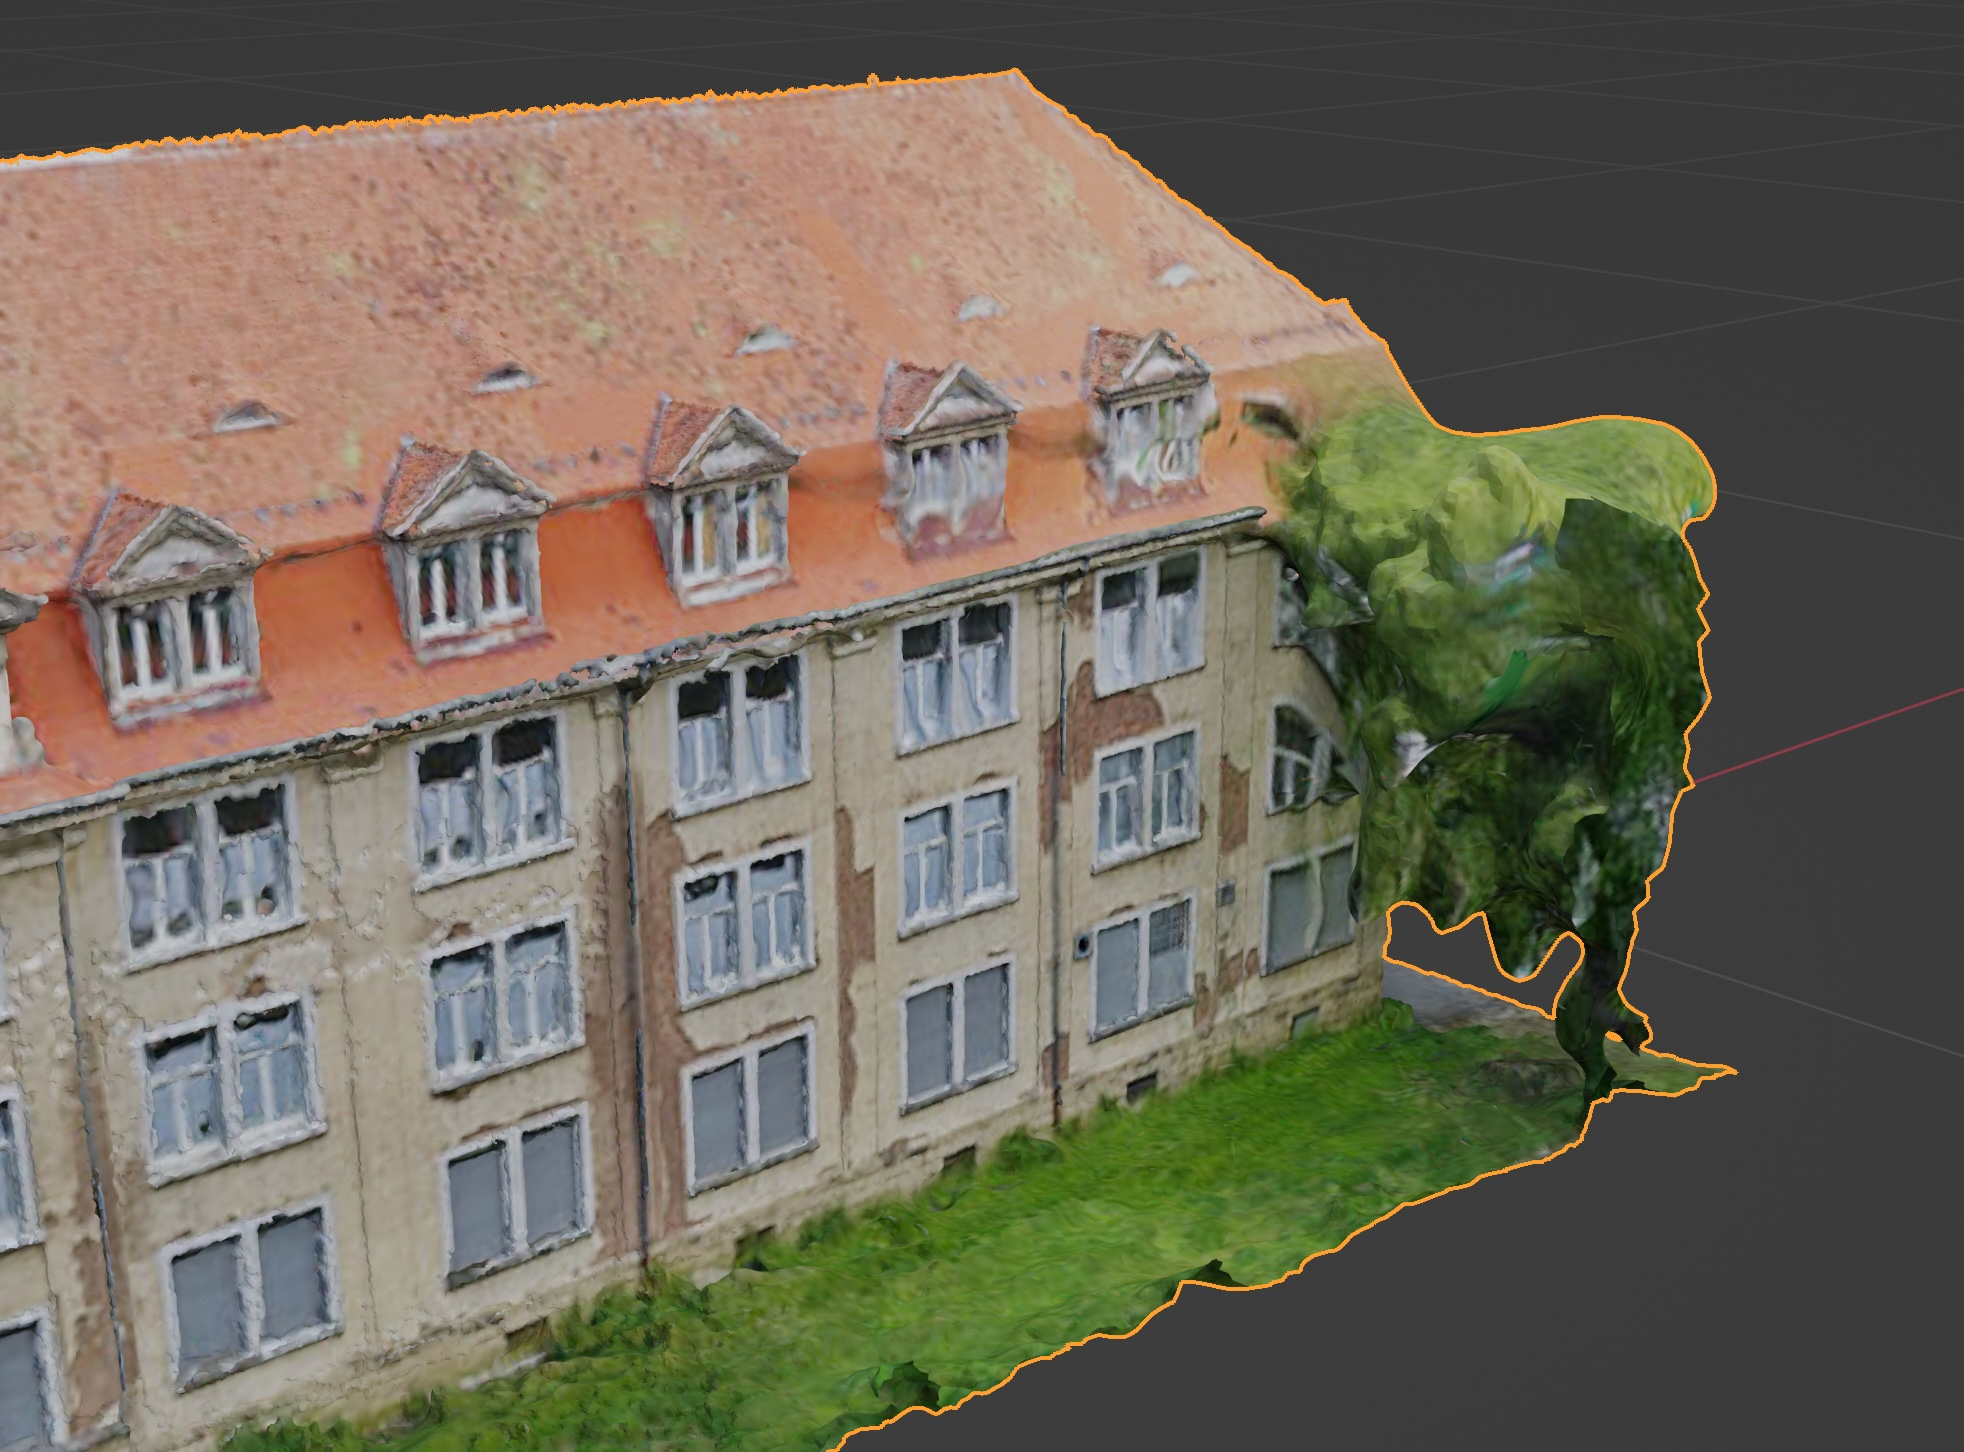
\includegraphics[width=0.5\textwidth]{img/vorbereitungen_blender_modelle/g2_verschmolzen.jpg}
    \caption{Ein Baum behinderte bei den Aufnahmen die Sicht auf die Wand, sodass diese mit dem Baum verschmolzen ist.}
    \label{fig:g2_verschmolzen}
\end{figure}

Zunächst wird das Modell kopiert. Anschließend werden die fehlerhaften Polygone im \textit{Edit-Mode} ausgewählt und gelöscht. Beim kopierten Modell werden alle Polygone gelöscht, bis auf die Wand, die eingesetzt werden soll. Diese wird mit dem \textit{Mirror-Modifier} gespiegelt. Das gespiegelte Modell wird an die Position der fehlerhaften Wand gesetzt und die beiden Modelle werden mit \textit{STRG + J} als ein Modell zusammengefügt. Die Lücke zwischen den beiden Modellen wird anschließend händisch mit neuer Geometrie gefüllt. Dieser Prozess ist sehr zeitaufwendig, da je nach Polygonanzahl viele Kanten einzeln ausgewählt werden müssen. Daher wird zunächst ein \textit{Decimate-Modifier} benutzt, um die Anzahl an Polygone zu reduzieren. Bei diesem Gebäude wird eine Reduzierung um 70\% vorgenommen, sodass sich die gesamte Anzahl an Polygonen von über 2.5 Millionen auf ca 750.000 Polygone verringert, ohne einen starken Verlust im Detailgrad festzustellen.

\begin{figure}[hbt!]
    \centering
    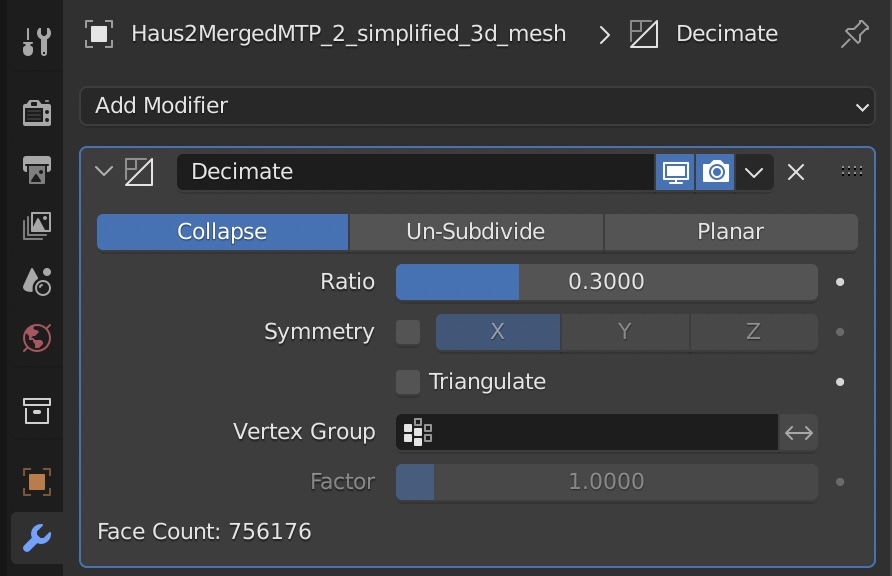
\includegraphics[width=0.5\textwidth]{img/vorbereitungen_blender_modelle/blender_decimate.jpg}
    \caption{Der Decimate-Modifier reduziert die Anzahl an Polygonen. Ein Wert von 0.3 beduetet, dass die Polygonenanzahl 30\% der ursprünglichen Polygonanzahl entspricht.}
    \label{fig:blender_decimate_modifier}
\end{figure}

Um die Lücken zu schließen werden benachbarte Kanten im \textit{Edit-Mode} ausgewählt und mit der \textit{F-Taste} mit neuen Flächen aufgefüllt. An einigen Stellen sind kleine Polygone vorhanden, bei dem dieser Prozess erschwert wird. Diese werden gelöscht und mit größeren Flächen ersetzt.  

\begin{figure}[hbt!]
    \centering
    \subfloat[][]{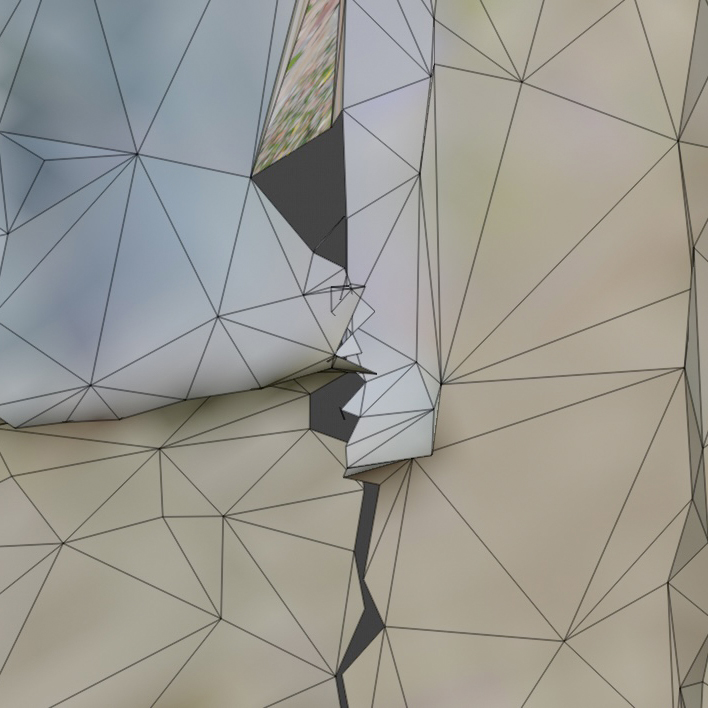
\includegraphics[width=0.4\linewidth]{img/vorbereitungen_blender_modelle/kleine_polygone_entfernen_1.jpg}}%
    \qquad
    \subfloat[][]{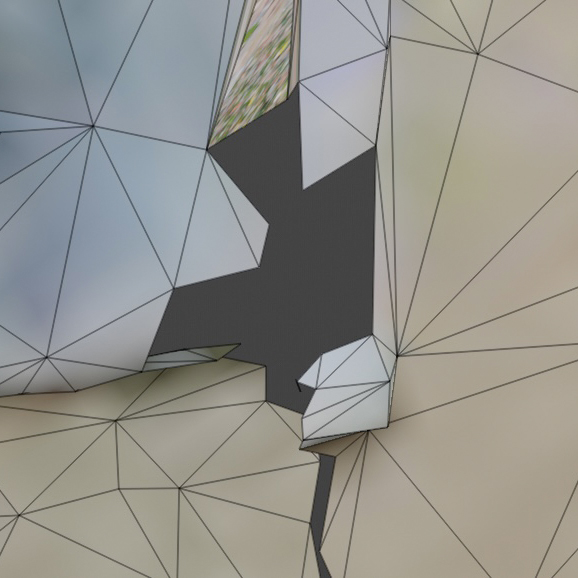
\includegraphics[width=0.4\linewidth]{img/vorbereitungen_blender_modelle/kleine_polygone_entfernen_2.jpg}}%
    \caption{Kleine Polygone erschweren das Markieren von Kanten (a). Das entstandene Loch wird mit größeren Flächen gefüllt (b).}%
    \label{fig:blender_kleine_polygone}
\end{figure}

\begin{figure}[hbt!]
    \centering
    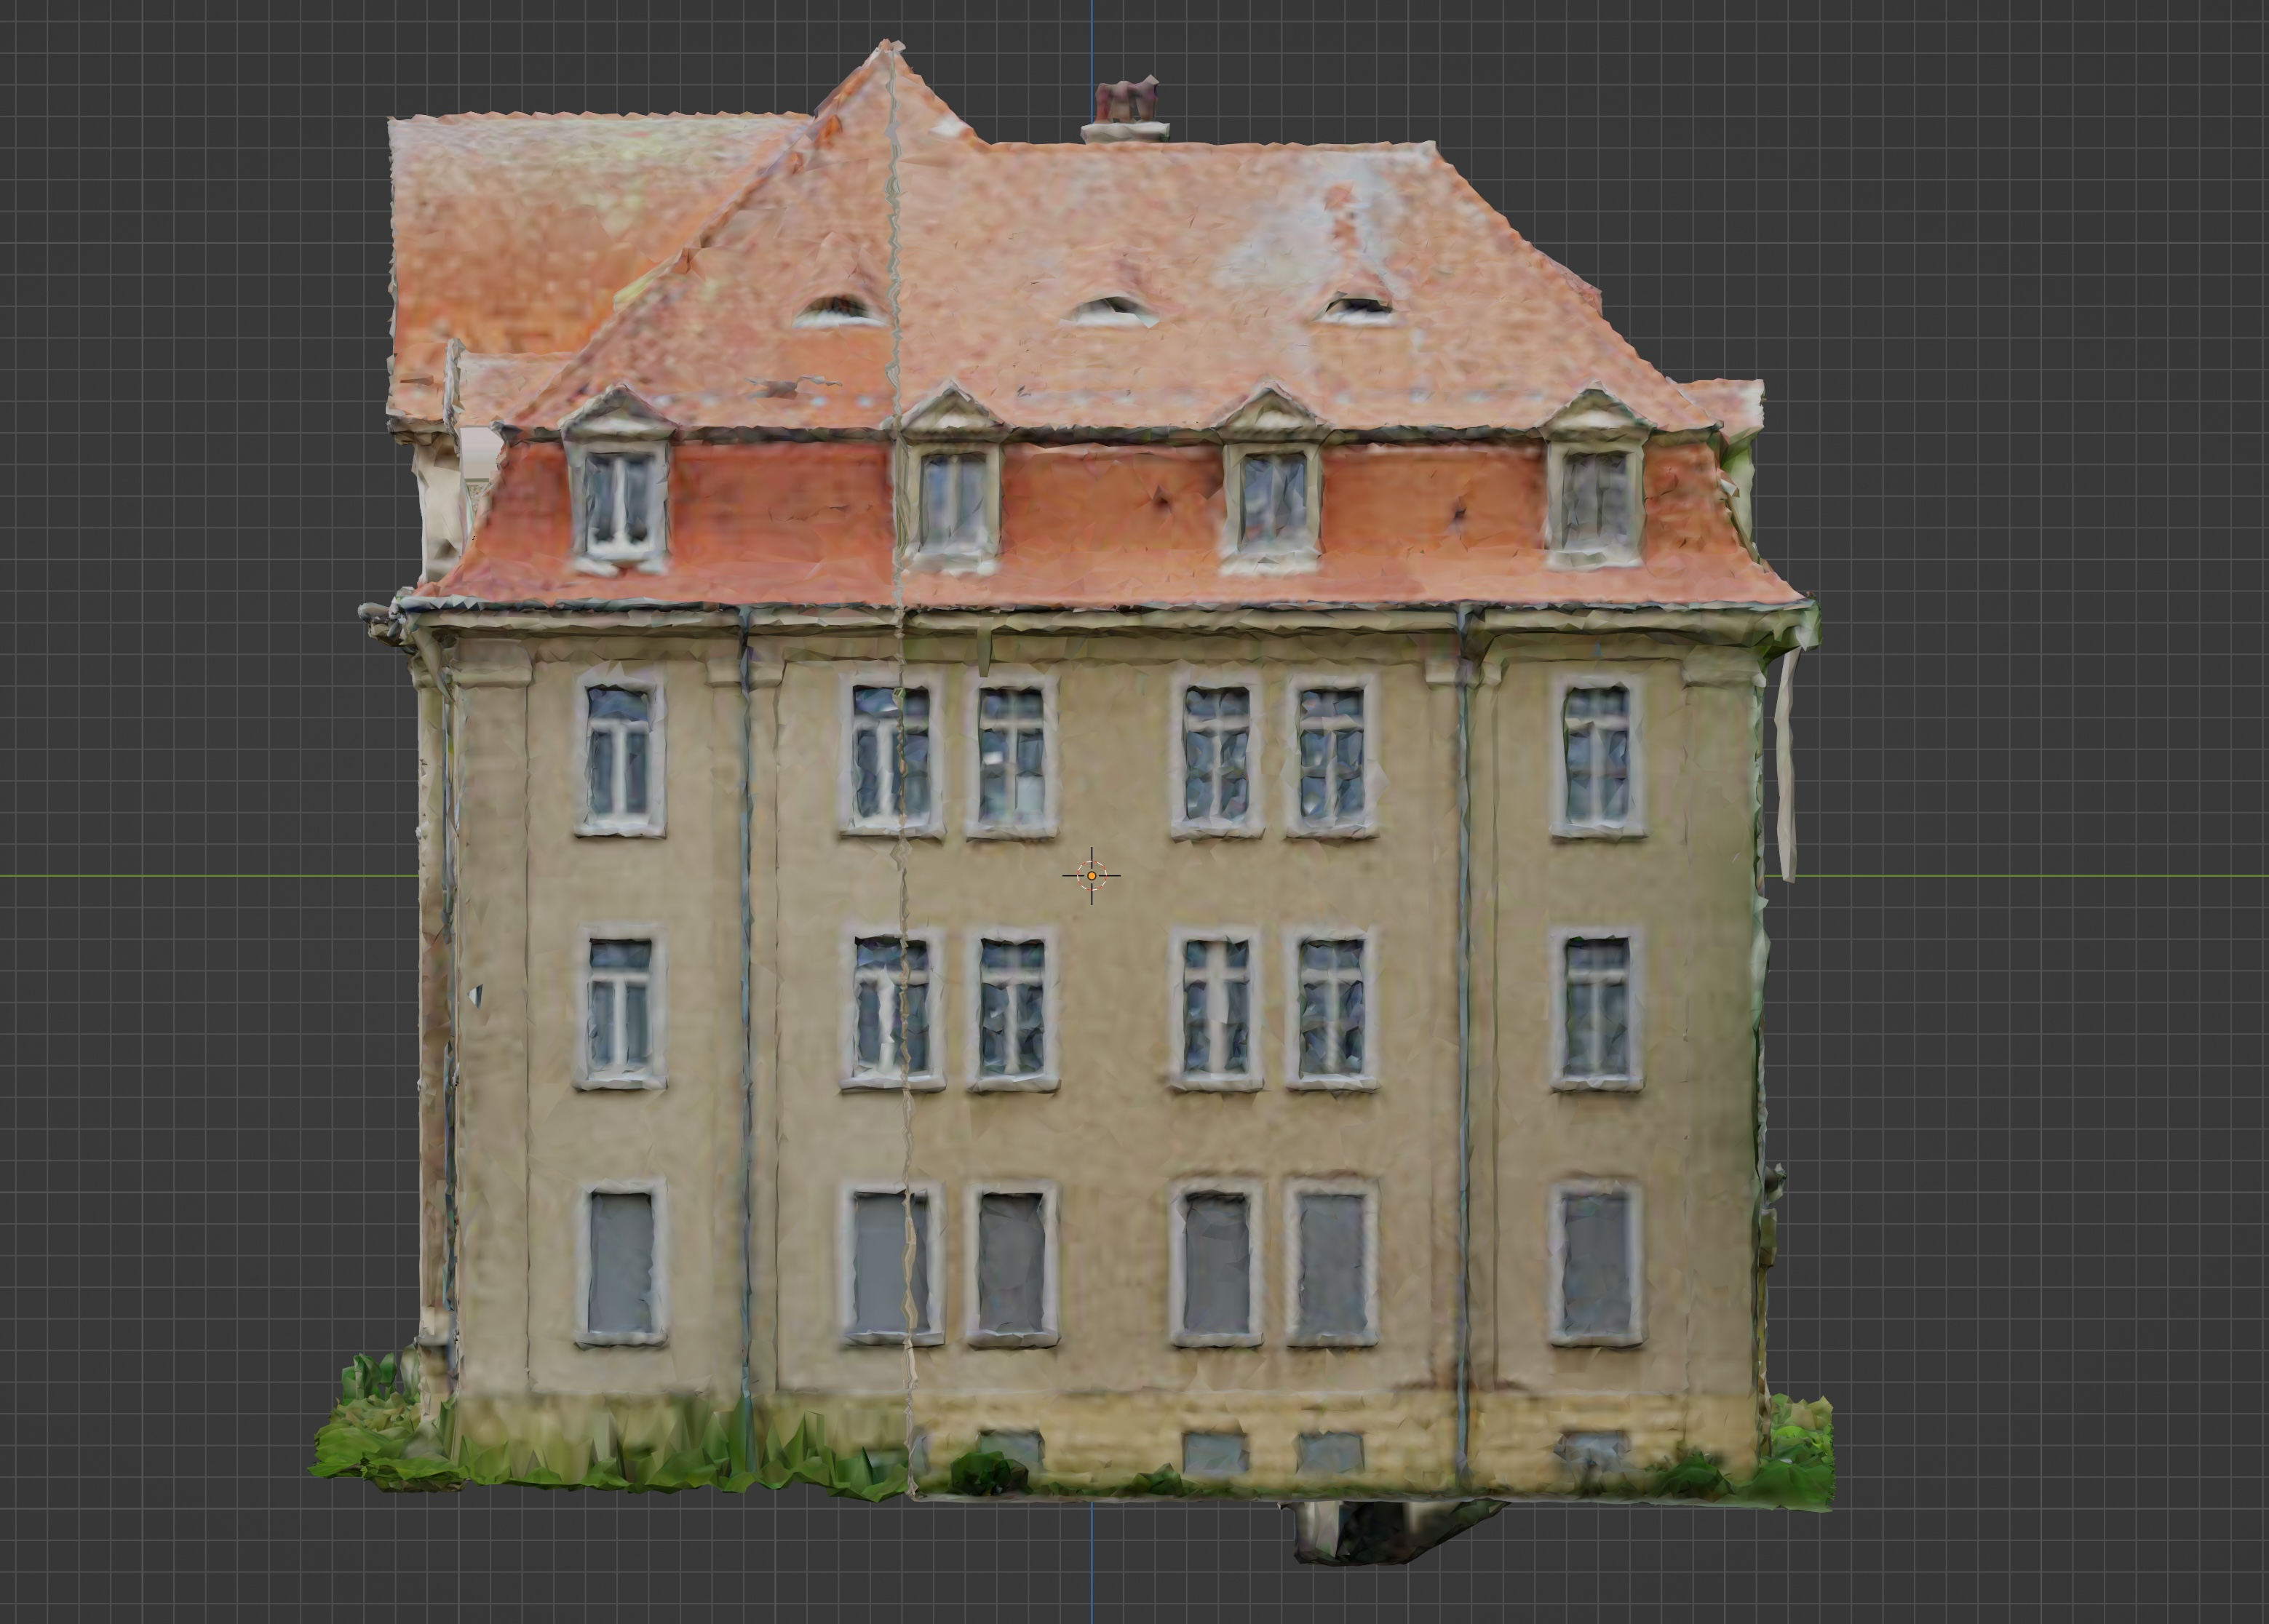
\includegraphics[width=0.5\textwidth]{img/vorbereitungen_blender_modelle/g2_naht.jpg}
    \caption{Das zusammengesetzte Gebäude.}
    \label{fig:blender_naht}
\end{figure}

Ist der Füllprozess abgeschlossen, ist die Naht dennoch erkennbar (siehe Abbildung \ref*{fig:blender_naht}), da die Textur auf den neuen Polygonen verzerrt wird. Aufgrunddessen werden im letzten Schritt im UV-Editing Tab die UV-Koordinaten der neuen Polygone neu vergeben, sodass die Texturen den umliegenden Flächen entsprechen. Hierfür werden die neuen Polygone im \textit{Edit-Mode} markiert. Im \textit{UV-Editor} werden mit dem Befehl \textit{U + Unwrap} die markierten Polygone bestmöglich auf die 2D Textur gelegt.\footnote{https://docs.blender.org/manual/en/latest/modeling/meshes/editing/uv.html, zuletzt augerufen am 29.05.2022} Die Polygone werden auf der Textur so skaliert, bewegt und rotiert, dass sie eine ähnliche Textur wie die umliegenden Flächen besitzen. Zur Hilfe werden die umliegenden Flächen markiert und deren UV-Koordinaten auf der Textur verglichen. So wird sichergestellt, dass die Farbunterschiede an den Kanten nicht zu stark abweichen. Das fertige Modell ist im Vorher-Nachher-Vergleich in Abbildung \ref*{fig:blender_vergleich} zu sehen. 

\begin{figure}[hbt!]
    \centering
    \subfloat[][]{\includegraphics[width=0.4\linewidth]{img/vorbereitungen_blender_modelle/polygone_markieren.jpg}}%
    \qquad
    \subfloat[][]{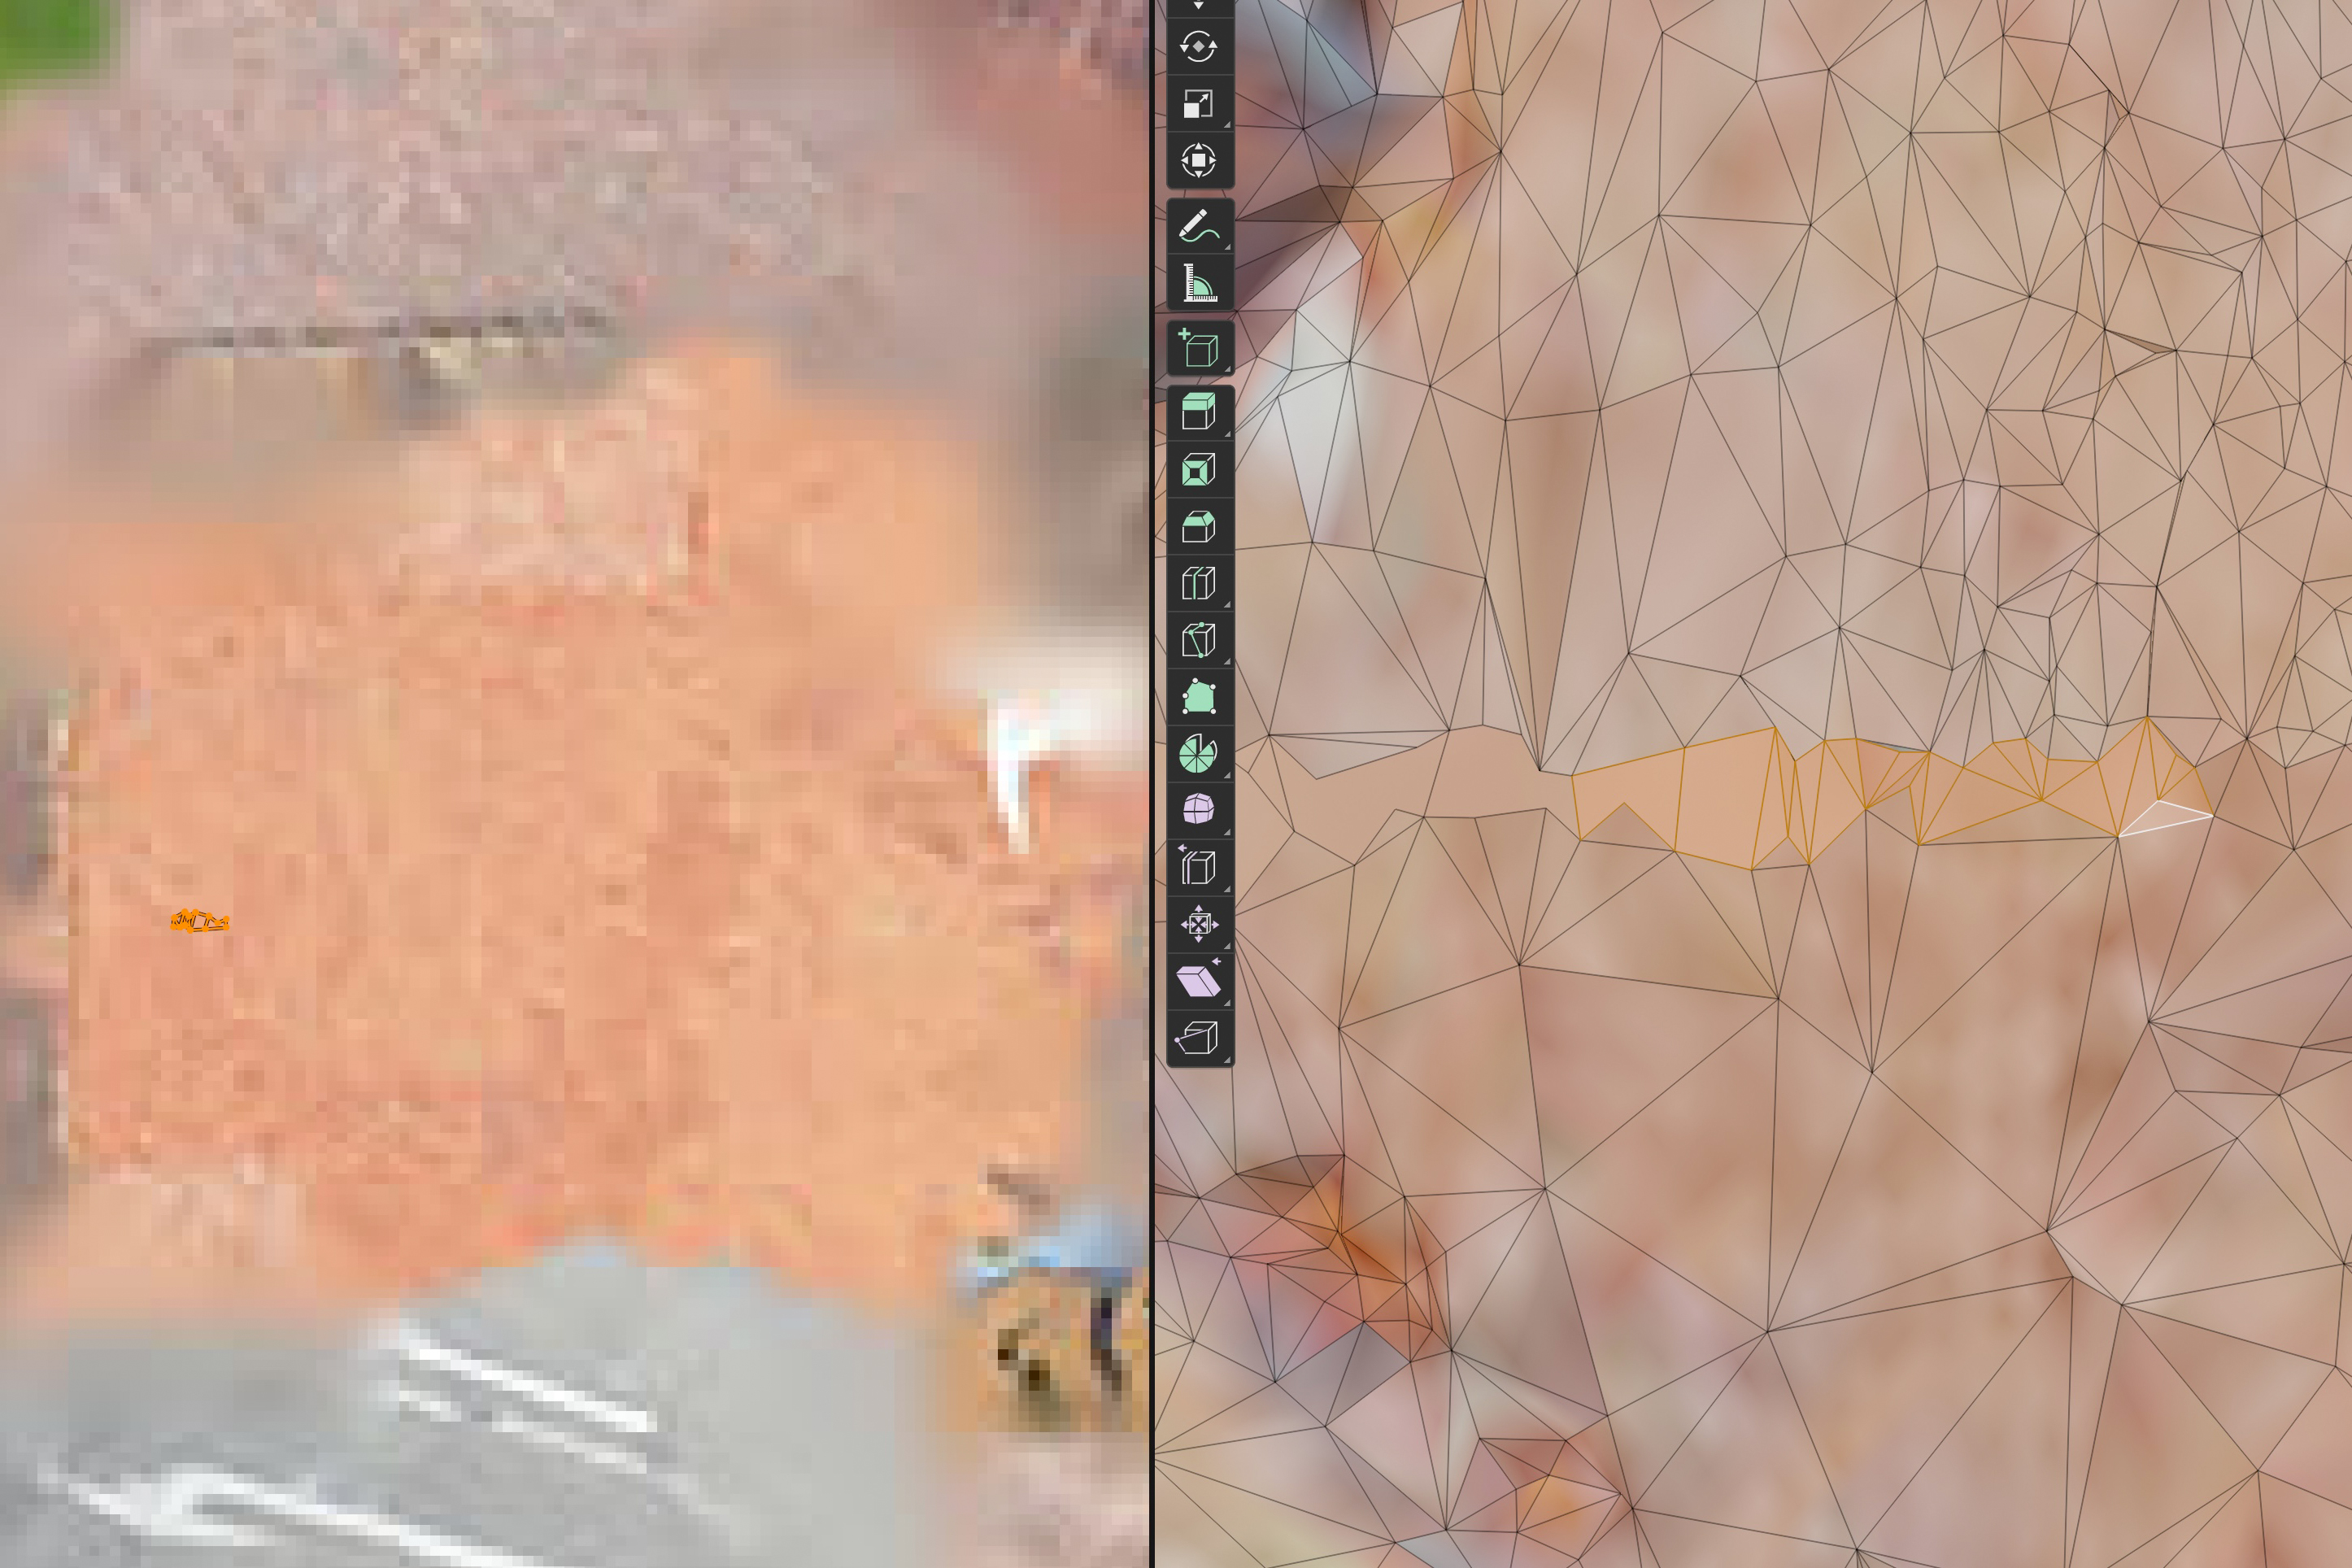
\includegraphics[width=0.4\linewidth]{img/vorbereitungen_blender_modelle/polygone_textur.jpg}}%
    \caption{Die Polygone werden markiert(a), unwrapped und anschließend auf eine geeignete Fläche auf der Textur gelegt(b).}%
    \label{fig:blender_uv_editing}
\end{figure}

\begin{figure}[hbt!]
    \centering
    \subfloat[][]{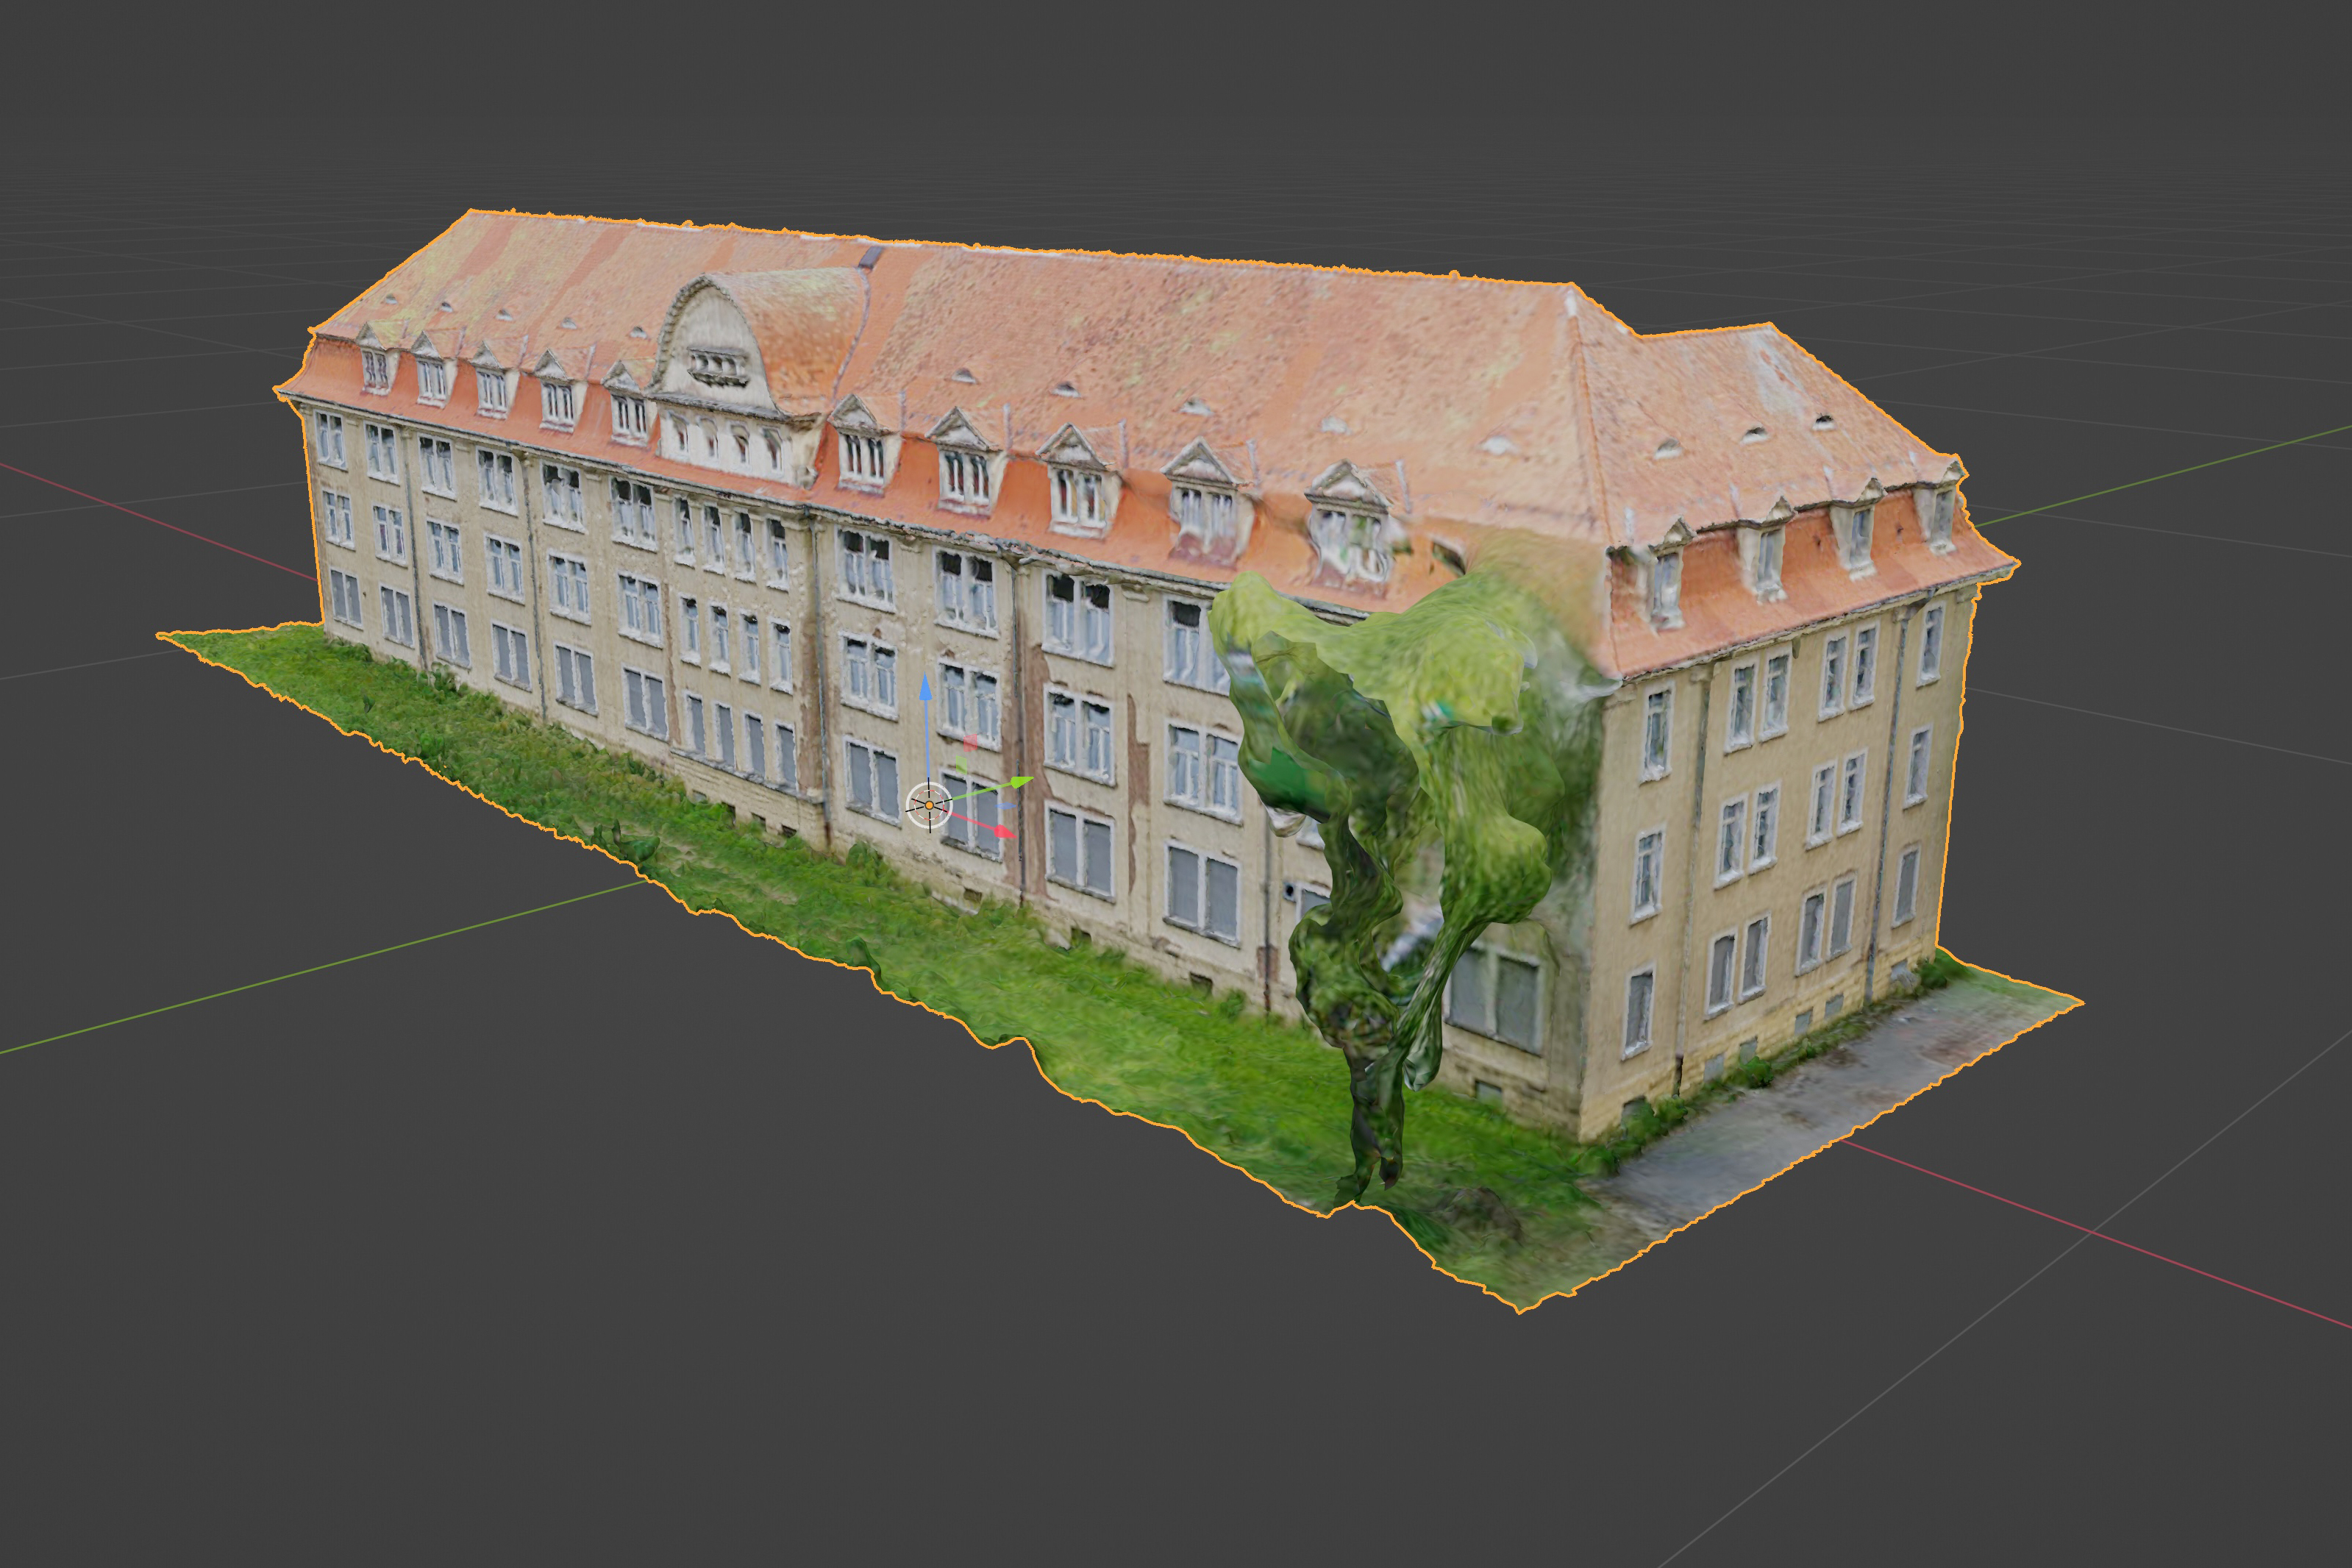
\includegraphics[width=0.4\linewidth]{img/vorbereitungen_blender_modelle/blender_vorher.jpg}}%
    \qquad
    \subfloat[][]{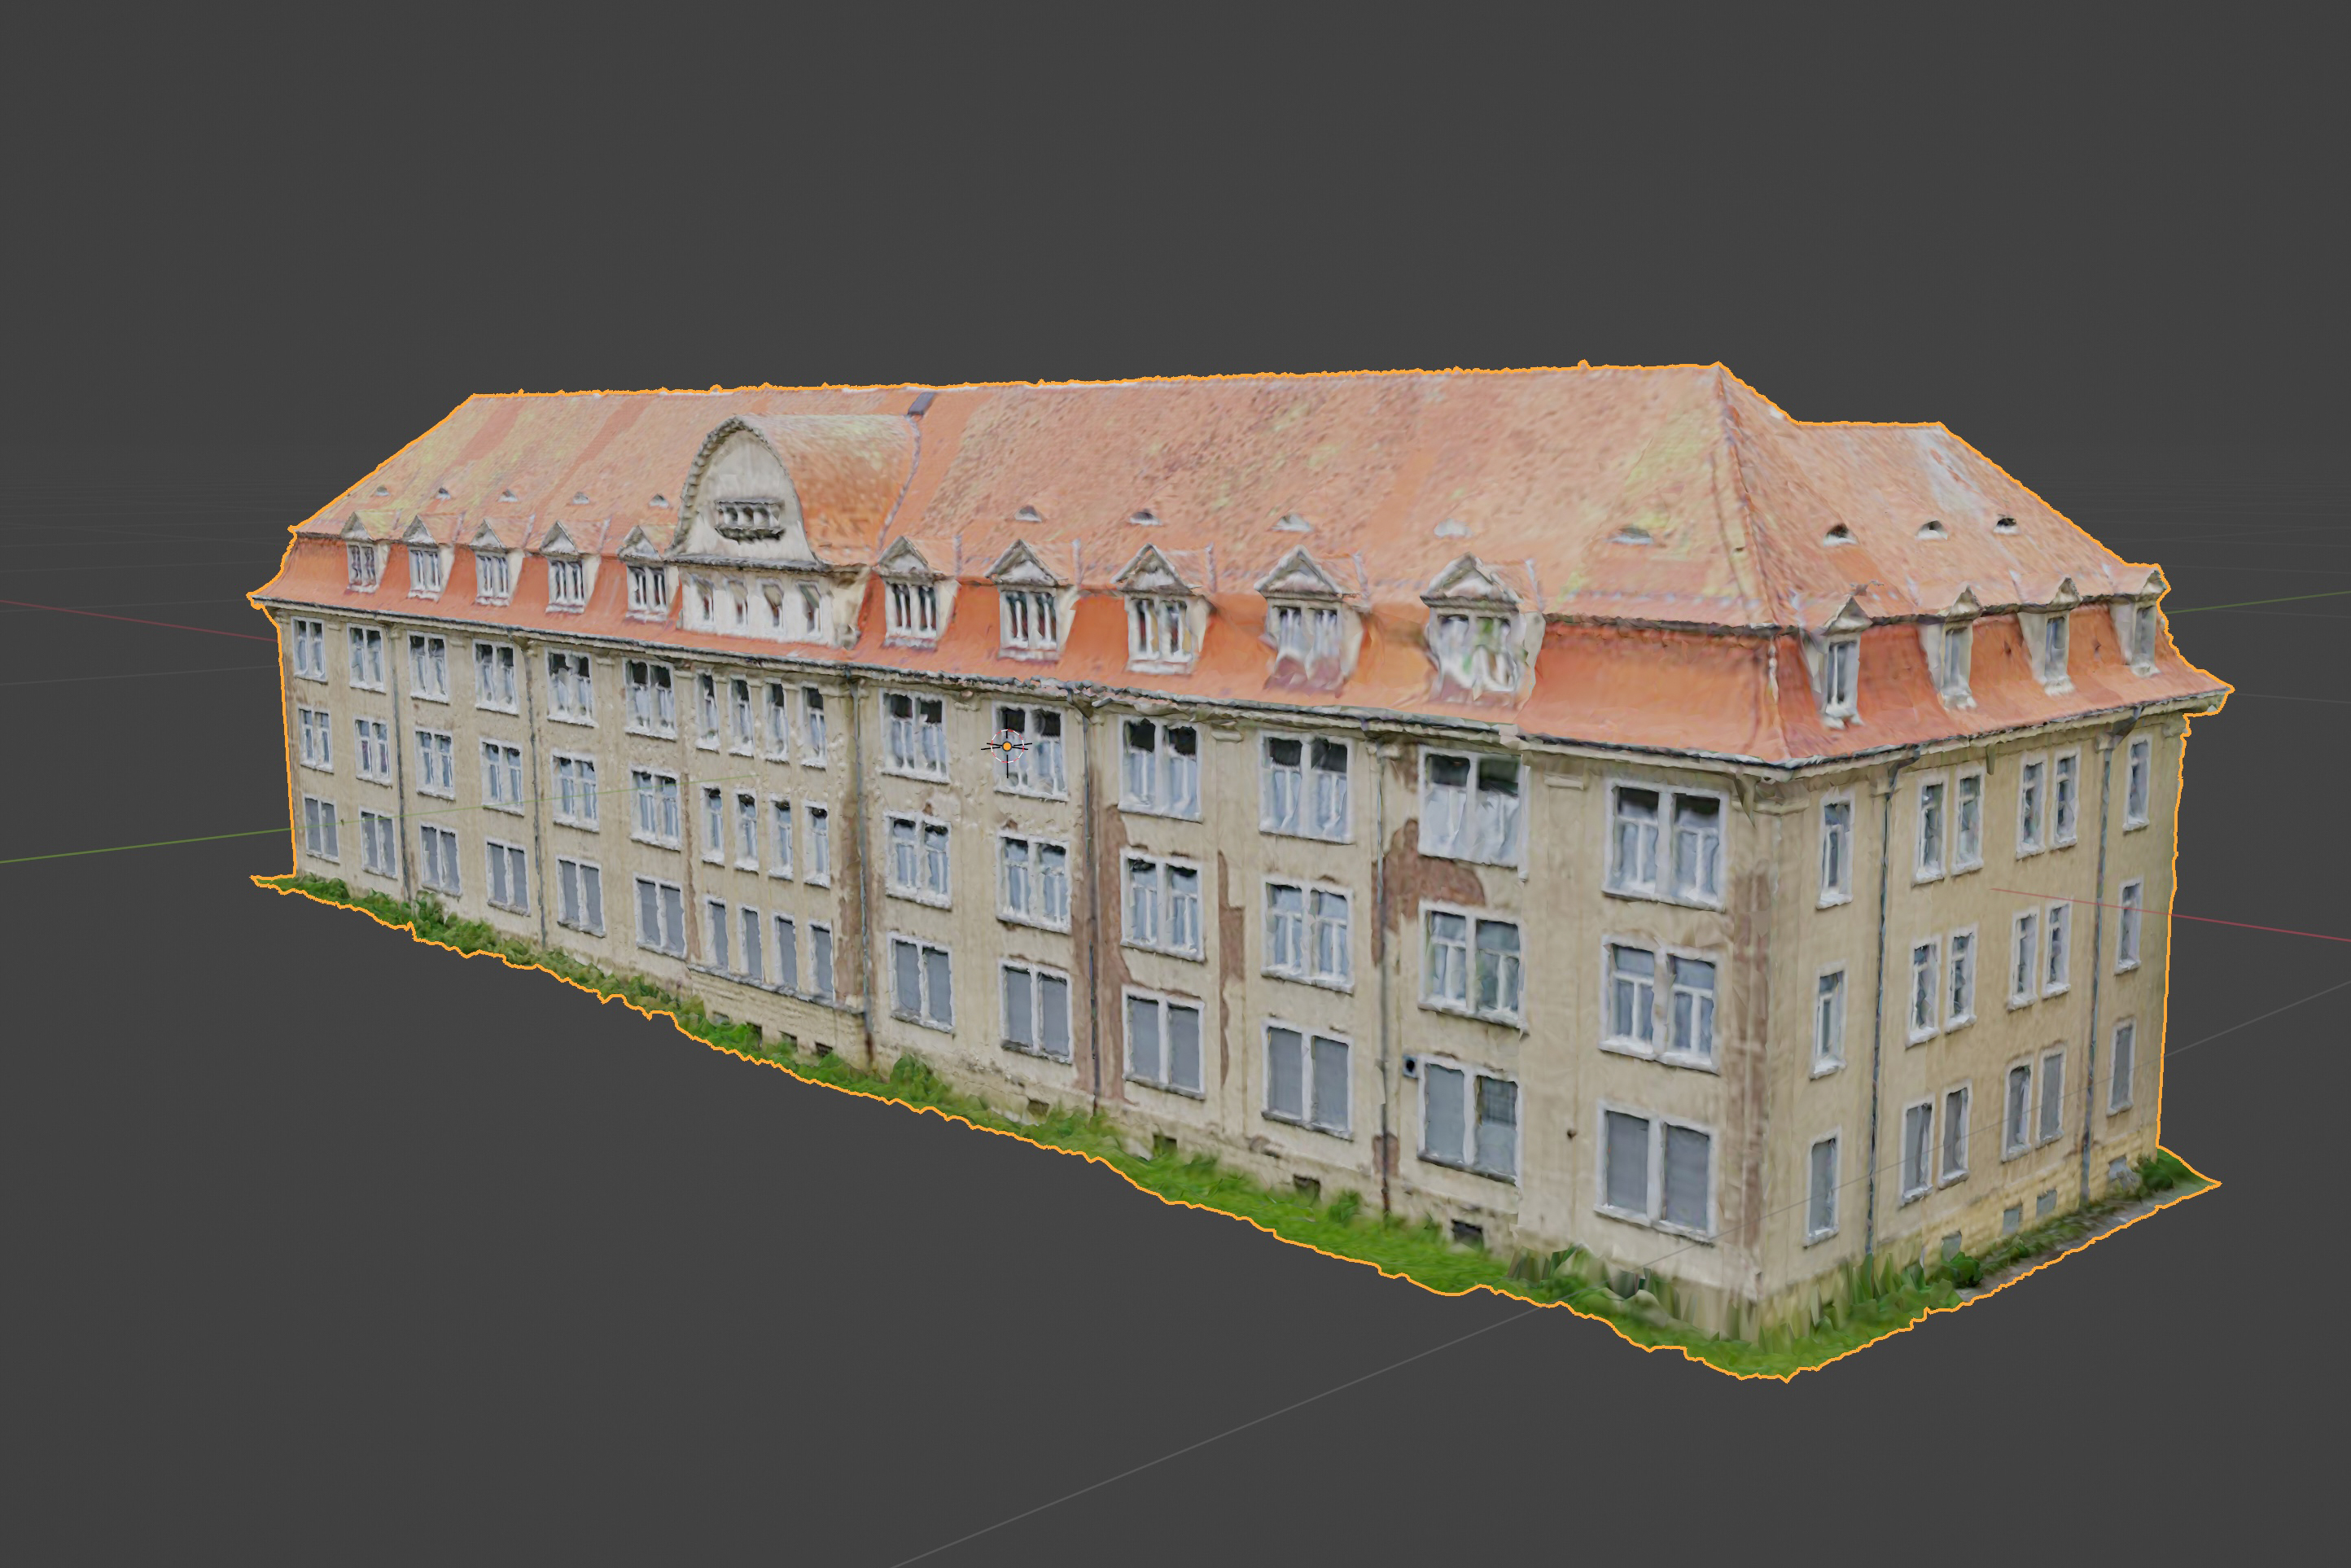
\includegraphics[width=0.4\linewidth]{img/vorbereitungen_blender_modelle/blender_nachher.jpg}}%
    \caption{Das Mannschaftsgebäude vor(a) und nach der Bearbeitung(b).}%
    \label{fig:blender_vergleich}
\end{figure}

\subsection{Export und Import}
Damit Unity die 3D Modelle korrekt darstellen kann, werden Anpassungen in Blender vorgenommen:

\begin{itemize}
    \item Vor dem Export werden Texturen in einem Ordner gespeichert. In Blender muss dafür die Option unter \textit{File>External Data>Automatically Pack Resources} ausgeschaltet sein. Anschließend wird mit \textit{File>External Data>Unpack Resources} ein Ordner im Projekt mit den Namen \textit{textures} erstellt, in dem sich die Texturen des Projekts befinden. Nun kann Unity die fehlenden Materials und Texturen im Projekt-Ordner finden,
    \item Unity kann die Texturen nur anwenden, wenn die Textur direkt im \textit{Shader Node} als \textit{Base Color} verbunden ist. Dazwischen befindliche Knoten funktionieren nur in Blender und müssen entfernt werden,
    \item die in Blender genutzten \textit{Modifier}\footnote{https://docs.blender.org/manual/en/latest/modeling/modifiers/index.html} werden angewendet,
    \item damit die Textur korrekt dargestellt werden, werden die Richtungen der \textit{Normalen}\footnote{https://docs.blender.org/manual/en/latest/modeling/meshes/editing/mesh/normals.html?highlight=normals} überprüft, ob diese in die richtige Richtung zeigen. Die Normalen müssen zur korrekten Darstellung nach außen zeigen. In Blender können die Normalen im \textit{Edit Mode} im Viewport Overlay angezeigt und unter \textit{Mesh>Normals} angepasst werden,
    \item Blender und Unity haben unterschiedliche Koordinatensysteme. In Blender zeigt die Z-Achse nach oben und die Y-Achse in die Tiefe, während in Unity die Y-Achse nach oben und die Z-Achse in die Tiefe zeigt. Damit die Modelle aus Blender mit der korrekten Orientierung dargestellt werden, wird das Modell in Blender um -90° gedreht. Mit \textit{STRG + A} und \textit{Rotation} wird die Rotation eingebettet,
    \item beim Export wird das Export-Format \textit{.fbx} benötigt.
\end{itemize}

Jetzt wird das 3D Modell als \textit{.fbx} Datei in Unity importiert. Im \textit{Inspector}-Fenster der \textit{.fbx} Datei werden unter Materials mit \textit{Exctract Materials} Materials in Unity generiert, die die Texturen beinhalten. Der Texturen-Ordner muss im gleichen Ordner liegen. Werden die Texturen nicht gefunden, so können diese händisch in das Projekt eingefügt werden. Um die Texturen den von Unity generierten Materials zu geben, wird im \textit{Inspector} die Textur in das Feld neben \textit{Albedo} eingefügt werden.
% - ARCore
% -- Features
\section{Technische Umsetzung}
\label{technische-umsetzung}
Dieses Kapitel erläutert, mit welcher Software und Hardware die Anwendung entwickelt wird. Damit wird ein Überblick geschaffen, welche Funktionen die Anwendung verwendet und wie die Implementierung durchgeführt wird. Es werden die Vorteile in der Entwicklung mit Unity und ARCore aufgeführt, um die Wahl der Software zu begründen. Anschließend werden die Funktionen von ARCore vorgestellt. 

Es wird der Aufbau der AR Szene und dessen Grundelemente erklärt, um einen Überblick zu erhalten, welche Elemente in der Szene bestimmte Funktionen ausführen. Die Implementierung der verwendeten ARCore Funktionen in dieser Anwendung wird kurz erläutert, um den State of the Art der Entwicklung von AR näher zu bringen. Im Anschluss erfolgt eine Bewertung der Funktionen. Die Kriterien dafür sind die Nutzbarkeit für diese Anwendung und inwiefern die jeweilige Funktion die Nutzererfahrung erweitert.

Danach wird veranschaulicht, wie die Anbindung zu Open Weather Map umgesetzt wird und wie eine Antwort der API aussieht. Die Implementierung der Anpassungen an die verschiedenen Wetterbedingungen wird im Code gezeigt. Um die Veränderungen in der Erscheinung der Gebäude nachzuvollziehen, werden die Ergebnisse miteinander verglichen.

\subsection{Verwendete Software und Hardware}
\label{technsich-umsetzung-verwendete-software-hardware}
Diese AR Anwendung wird mit Unity\footnote{https://unity.com/} in der Version \textit{2021.2.14} und AR Foundation\footnote{https://unity.com/de/unity/features/arfoundation} in der Version \textit{4.2.2} entwickelt. Unity ist eine Spiel-Engine, die eine Laufzeit- und Entwicklungsumgebung für Spiele und 3D Grafik Anwendungen bietet. Unity ist überwiegend kostenlos. Es gibt kostenpflichtige Unity Komponenten, die für diese Arbeit nicht relevenat sind. AR Foundation ist ein Framework von Unity für die Entwicklung von Augmented-Reality Anwendungen. Mit AR Foundation werden offiziell Plug-Ins für Googles ARCore, ARKit und weiteren Mixed Reality SDK's für Unity angeboten. Die Nutzung von Unity und AR Foundation bietet diverse Vorteile, die im folgenden Abschnitt erläutert werden. Aufgrund dieser Vorteile wird in dieser Arbeit auf die Entwicklung mit unity und ARFoundation gesetzt.

Das verwendete Smartphone ist ein Oneplus A6003\footnote{https://de.wikipedia.org/wiki/OnePlus\_6, zuletzt aufgerufen am 11.08.2022} aus dem Jahr 2018. Das Gerät läuft mit der Android Version 11 und der OxygenOS-Version 11.1.2.2.

\paragraph*{Entwicklungsumgebung}
Die Benutzeroberfläche von Unity ist verständlich und übersichtlich gestaltet. Der Einstieg wird dadurch vereinfacht. Funktionen und Packages von Unity können auch für AR Anwendungen genutzt werden. Beispielsweise wird die Erstellung des User-Interface vereinfacht. Durch die Nutzung von einzelnen Szenen wird die Wahl der Positionierung (GPS oder lokal auf einer Fläche) umgesetzt und es können Buttons, Texte und Slider mit den jeweiligen Interaktionen verwendet werden. Dies beschleunigt den Entwicklungsprozess und der Fokus der Arbeit kann mehr auf die Umsetzung der Licht und Wetterveränderung gesetzt werden.

\paragraph*{Kompatibilität}
Unity kann für viele verschiedene Plattformen genutzt werden. Neben den Plattformen für die Spieleentwicklung, ist es möglich sowohl für Android als auch für iOS zu entwickeln. Auch bietet sich eine große Auswahl an Augmented Reality \acrshort{sdk}'s. Neben ARCore\cite*{ARCore} und ARKit\cite*{ARKit} ist es z.B. möglich Vuforia\cite*{Vuforia}, Wikitude\cite*{Wikitude} oder ARToolkit\cite{ARToolkit} zu verwenden. Hierfür werden Plug-Ins des jeweiligen Anbieters benötigt. Der Vorteil von ARFoundation ist die offizielle Plug-In Unterstütztung für ARCore und ARKit. Die Plug-Ins werden regelmäßig geupdatet und die Implementierung ist einfach gestaltet. Diese Vielfältigkeit der Plattformauswahl ist in Hinblick auf die Zielgruppe ein Vorteil. So ist die Anwendung nicht auf ein Betriebssystem wie Android oder iOS beschränkt und es können dadurch mehr Nutzer die App ausprobieren.

\paragraph*{Dokumentation}
Die Unity Dokumentation\cite*{UnityARFoundation} ist ausführlich. Die Funktionen von ARCore und ARKit werden vorgestellt. Die Installation der benötigten Packages und der Szenenaufbau einer AR Anwendung wird erklärt. Neben der Dokumentation für die AR-spezifischen Funktionen gibt es eine umfangreiche Dokumentation für die Nutzung von Unity selbst\footnote{https://docs.unity3d.com/2023.1/Documentation/Manual/index.html, zuletzt aufgerufen am 09.08.2022}. Damit wird der Einstieg in die Entwicklungsumgebung vereinfacht und die Implementierung von Funktionalitäten kann anhand der gegebenen Beispielen in der Dokumentation besser nachvollzogen werden.

\paragraph*{Programmiersprache C\# und die große Community}
Unity verwendet die Programmiersprache C\#\footnote{https://docs.microsoft.com/de-de/dotnet/csharp/tour-of-csharp/, zuletzt aufgerufen am 09.08.2022}, die laut PYPL-Index im August 2022 hinter Python, Java und JavaScript als viertbeliebteste Programmiersprache gilt\cite*[PYPL,][]{PYPLStatista2022}. Damit kann während der Entwicklung auf die Erfahrung von anderen Nutzern zurückgegriffen werden, wenn es Probleme gibt. Auch ist eine ausführlichen Dokumentation vorhanden. Da im Studiumsverlauf bereits mit C\# gearbeitet wurde, fällt zudem der persönliche Einstieg leicht.

\paragraph*{Asset Store}
Unity bietet im Asset Store\footnote{https://assetstore.unity.com/, zuletzt aufgerufen am 09.08.2022} eine Vielfalt an kostenfreien und kostenpflichtigen Modellen und Skripten, die den Entwicklungsprozess beschleunigen. Anstatt Funktionen mit hohen Aufwand selbst zu schreiben, wird auf den Asset Store zurückgegriffen. Es wird nicht nur Zeit eingespart, sondern auch Fehler in der Entwicklung minimiert. In der Regel werden die veröffentlichten Skripte getestet und regelmäßig mit Bug-fixes verbessert. Damit wird die Fehleranfälligkeit minimiert und der Nutzer hat ein besseres Benutzererfahrung. Im Kapitel \ref*{technische-umsetzung-licht} wird beispielsweise die Positionierung der Sonne vereinfacht implementiert.

\subsection{ARCore SDK}
\label{technische-umsetzung-arcore}
Ein \acrfull{sdk} ist eine Ansammlung von Entwicklungswerkzeugen, die zur Entwicklung von Software dient\footnote{https://de.wikipedia.org/wiki/Software\_Development\_Kit, zuletzt aufgerufen am 09.08.2022}. Sie beinhalten Softwarebibliotheken, -pakete und Frameworks, um die Entwicklung auf bestimmten Plattformen wie z.B. Smartphones oder Spielekonsolen zu ermöglichen. Softwareentwickler greifen auf diese Bibliotheken zu, um den Entwicklungsprozess zu beschleunigen. Mit \acrshort{sdk}'s werden z.B. Algorithmen bereitgestellt, die immer wieder gebraucht werden. In der Entwicklung für AR Anwendungen betrifft dies insbesondere das Tracking (Kapitel \ref*{tracking}).

Für AR gibt es mehrere SDK's, die für die Entwicklung von Smartphone Anwendungen geeignet sind. Diese sind z.B. ARCore\cite*{ARCore}, ARKit\cite*{ARKit}, Vuforia\cite*{Vuforia}, Wikitude\cite*{Wikitude} oder ARToolkit\cite*{ARToolkit}.

ARCore ist die AR Plattform von Google. Sie verwendet drei wichtige Funktionen, um virtuelle Inhalte in die reale Welt zu integrieren, die auch in dieser Anwendung eine wichtige Stütze für eine gute Nutzererfahrung sind: \textit{Motion Tracking}, \textit{Environmental understanding} und \textit{Light estimation}.

\subsubsection{Technische Voraussetzungen}
\label{technische-umsetzung-arcore-voraussetzungen}
ARCore kann von vielen Geräten mit Android 7.0 Nougat mit dem API Level 24 oder höher genutz werden. Auch iOS Geräte mit iOS 11.0 oder höher sind mit ARCore kompatibel. Lediglich die Tiefen-API wird nicht von allen Geräten unterstützt. Die Dokumentation von ARCore\cite*{ARCoreDokumentation} bietet eine Tabelle mit allen kompatiblen Geräten.

\subsubsection{Motion Tracking}
\label{technische-umsetzung-arcore-motion-tracking}
\textit{Motion-Tracking} ermittelt die Position und Orientierung des Smartphones im Bezug zur Umgebung. Laut der offiziellen Dokumentation\cite{ARCoreDokumentation} und dem Patent zu Googles AR Core\cite[][]{esha2017} wird ein \acrshort{slam} System genutzt. Es werden Schlüsselpunkte in der Umgebung identifiziert. Diese werden mit den Daten aus der \acrshort{imu} kombiniert, um die relative Position und Orientierung des Smartphones zum Weltkoordinatensystem zu bestimmen. Mit Motion Tracking ist nur die Ermittlung der Position und Orientierung des Smartphones gemeint. Die Erstellung der Karte von der Umgebung wird ähnlich zu \acrshort{ptam} von Klein und Murray\cite*{klein2007} getrennt. Die Karte wird in der Funktion \textit{Environmental understanding} erstellt.

\subsubsection{Environmental understanding}
\label{technische-umsetzung-arcore-environmental-understanding}
\textit{Environmental understanding} erkennt die Größe und die Position aller Oberflächen in der Umgebung. Damit werden Oberflächen wie Tische, Wände oder Böden erfasst. Die Umgebung wird im Laufe der Anwendung kontiniuerlich mit Schlüsselpunkten erweitert. Bestehende Schlüssselpunkte werden verbessert. Es wird eine Karte der Umgebung erzeugt, die aus Schlüsselpunkten besteht. AR Core ist dann dazu in der Lage zusammenhängende Schlüsselpunkte zu erkennen, um damit Flächen und Wände zu identifizieren. Es werden horizontale als auch vertikale Flächen erkannt.

Motion Tracking und Environmental understanding ist als Grundfunktion für diese Anwendung essentiell.

\subsubsection{Light estimation}
\label{technische-umsetzung-arcore-light-estimation}
ARCore schätzt Informationen über die Lichtverhältnisse in der realen Umgebung. Es werden \textit{lighting cues} in der Umgebung erkannt. Diese light cues beeinflussen die Farbe und die Helligkeit von jedem Pixel eines Bildes. Light cues sind:
\begin{itemize}
    \item das Ambient light. Das ist das diffuse Licht aus der Umgebung, 
    \item die Schatten bzw. Schattenwürfe, die Aufschluss darüber geben, aus welcher Richtung das Hauptlicht kommt,
    \item Shading, das die Intensität des Lichts bestimmt,
    \item spiegelnde Highlights. Diese entstehen, wenn das Licht direkt auf eine spiegelnde Fläche sheint,
    \item die Reflektionen von Objekten.
\end{itemize}

Light estimation hat zwei Modi: den \textit{Ambient Intensity mode} und den \textit{Environmental HDR Mode}.

\paragraph*{Ambient Intensity mode}
Dieser Modus ermittelt mit dem Bild der Kamera die durchschnittliche Helligkeit und die durchschnittliche Farbtemperatur der Umgebung. Das Hauptlicht erhält damit eine Einfärbung in das Umgebungslicht.

\paragraph*{Environmental HDR Mode} Dieser Modus nutzt zusätzliche APIs mit Machine Learning Algorithmen. Das Kamerabild wird dazu genutzt die Beleuchtung der Umgebung zu verstehen. Environmental HDR Mode basiert auf die Arbeiten von LeGendre et al.\cite*{LeGendre2019}. Dabei wird das Bild nach den Light cues analysiert. 

Environmental HDR berechnet drei Komponenten. Das \textit{Main directional light} ist das Hauptlicht, dass die reale Szene aufhellt. In Outdoor AR ist dies in der Regel die Sonne. Diese API berechnet die Richtung und die Intensität des Hauptlichtes. Mit dieser Information werden z.B. spiegelnde Highlights auf den Modellen berechnet. Außerdem wird die Intensität und die Richtung der Schatten angepasst. 

Zusätzlich zum Hauptlicht, werden \textit{Ambient spherical harmonics} berechnet. Sphärisch-harmonische Beleuchtung wird in Detail von Green\cite*[]{green2003} erklärt und ist eine Technik zur Berechnung von globaler Beleuchtung. Es wird aus dem Kamerabild Informationen zum Umgebungslicht berechnet, das zusätzlich zum Hauptlicht die Objekte beleuchtet.

Letztlich werden \textit{HDR Cubemaps} in Echtzeit erstellt. Eine Cubemap ist ein Panoramabild, das Bilder einer Umgebung enthält. Das Panoramabild wird auf die sechs Flächen eines Würfels verteilt. Diese Cubemap wird verwendet, um zum einen Reflektionen der Umgebung bereitszustellen. Damit erhalten stark reflektierende Objekte, wie z.B. Metall, eine Spiegelung der Umgebung. Zum anderen wird das Umgebungslicht simuliert\cite*[Szelsiki Seite 410ff., ][]{szeliski2022}. Dies sorgt dafür, dass virtuelle Objekte harmonischer in das Bild integriert werden. In Abbildung \ref*{fig:anwendung-arcore-environmental-hdr} wird das Ergebnis aller Komponenten gezeigt.

\begin{figure}[h]
    \centering
    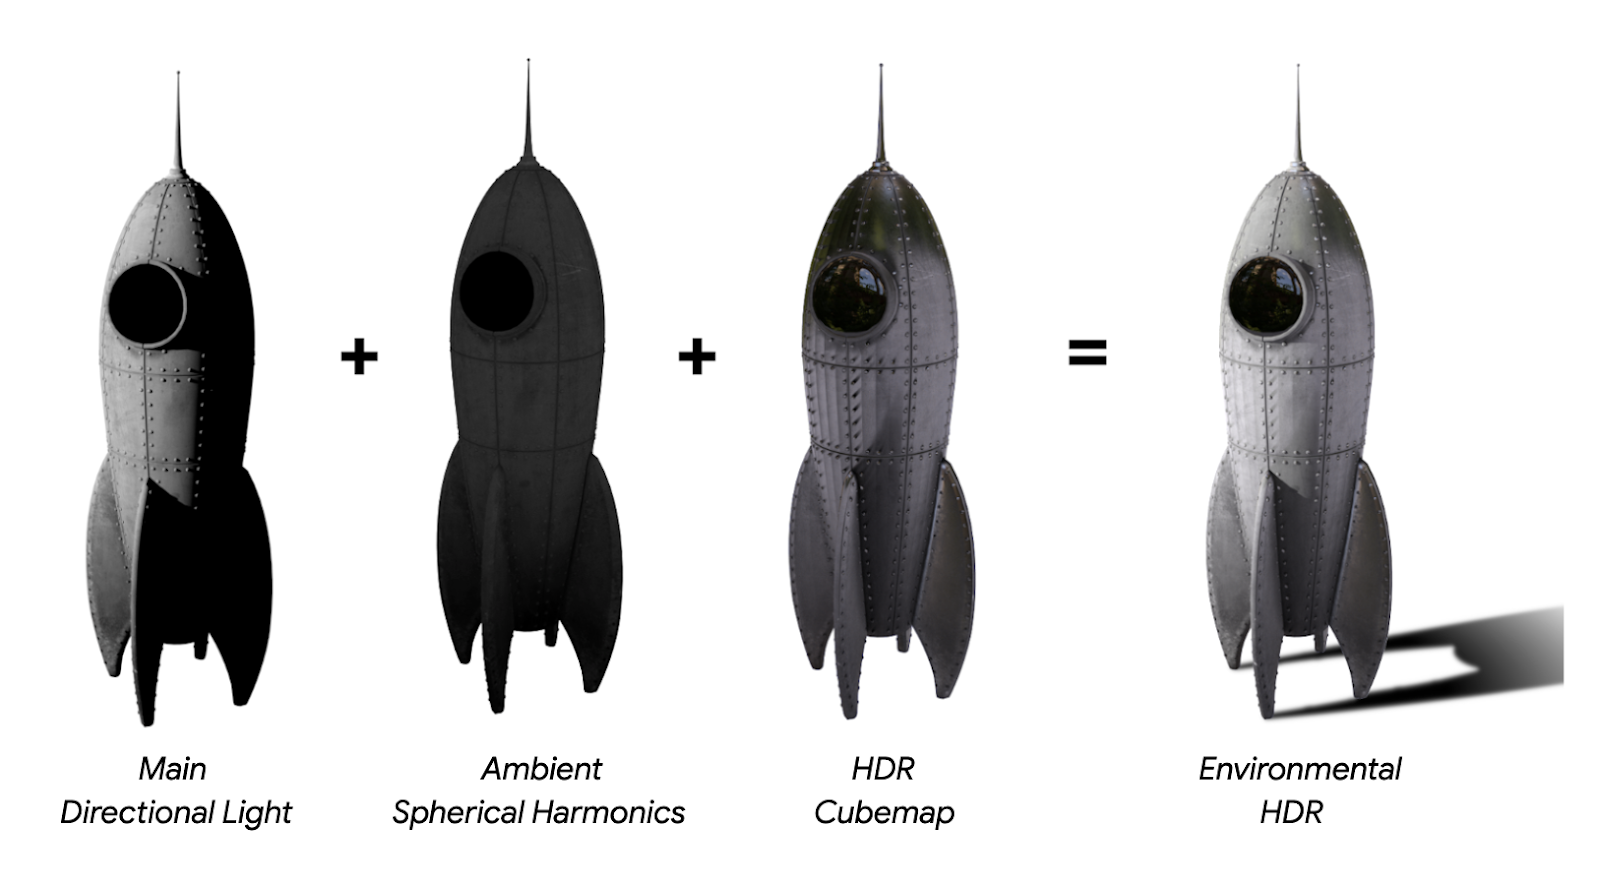
\includegraphics[width=\linewidth]{img/anwendung/arcore/arcore-light-estimation-environmentalhdr.png}
    \caption[Die Beleuchtungseinschaften und das kombinierte Endergebnis des Environmental HDR Modus.]{Die Beleuchtungseinschaften und das kombinierte Endergebnis des Environmental HDR Modus\protect\footnotemark.}
    \label{fig:anwendung-arcore-environmental-hdr}
\end{figure}
\footnotetext{Quelle Bild: https://developers.googleblog.com/2019/05/ARCore-IO19.html, zuletzt aufgerufen am 16.08.2022}

In dieser Arbeit wird dieser Modus verwendet, um die Reflektionen der Umgebung zu implementieren. Es werden in Kapitel \ref*{technische-umsetzung-licht} eigene Cubemaps aus Panoramabildern des SABA Gebäudes erstellt und benutzt. Dies ermöglicht das manuelle Einstellen der Wetterbedingungen. Damit wird in Kapitel \ref*{technische-umsetzung-wetterbedingungen} auch die Veränderung der Cubemaps sichtbar. 

Nachteil dabei ist, dass nur Cubemaps des SABA-Geländes genutzt werden. Da das SABA und Lyautey Gelände zum Zeitpunkt dieser Arbeit bebaut wird, verändert sich die Umgebung. Eine Erstellung von Cubemaps für jedes Gebäude würde sich demnach nicht lohnen, da sich der Ort verändert. Für eine weiterführende Arbeit wird daher empfohlen den Environmental HDR Mode zu verwenden. Die Cubemaps für die Reflektionen und das Environmental Lighting wird sich dann an den realen Gegebenheiten anpassen.

\subsubsection{User Interaction}
\label{technische-umsetzung-arcore-user-interaction}
Um Interaktionen des Nutzers zu den virtuellen Objekten zu implementieren, wird \textit{hit-testing} durchgeführt. In AR Foundation bzw. Unity wird dies \textit{Raycast} genannt. Daher wird diese Funktion nicht mit ARCore, sondern mit Unity implementiert. Das Prinzip ist gleich. Beim hit-testing wird ein virtueller Strahl vom Smartphone aus in die Umgebung erzeugt. Es werden Schnittpunkte zwischen diesen Strahl und virtuellen Objekten gefunden. Das \textit{Hit-Ergebnis} beinhaltet drei Informationen:

\begin{itemize}
    \item die Distanz des Smartphones zum Objekt, 
    \item die Position und die Orientierung des hits im Weltkoordinatensystem,
    \item die 3D Gemoetrie des getroffenen Objekts.
\end{itemize}

\begin{figure}[h]
    \centering
    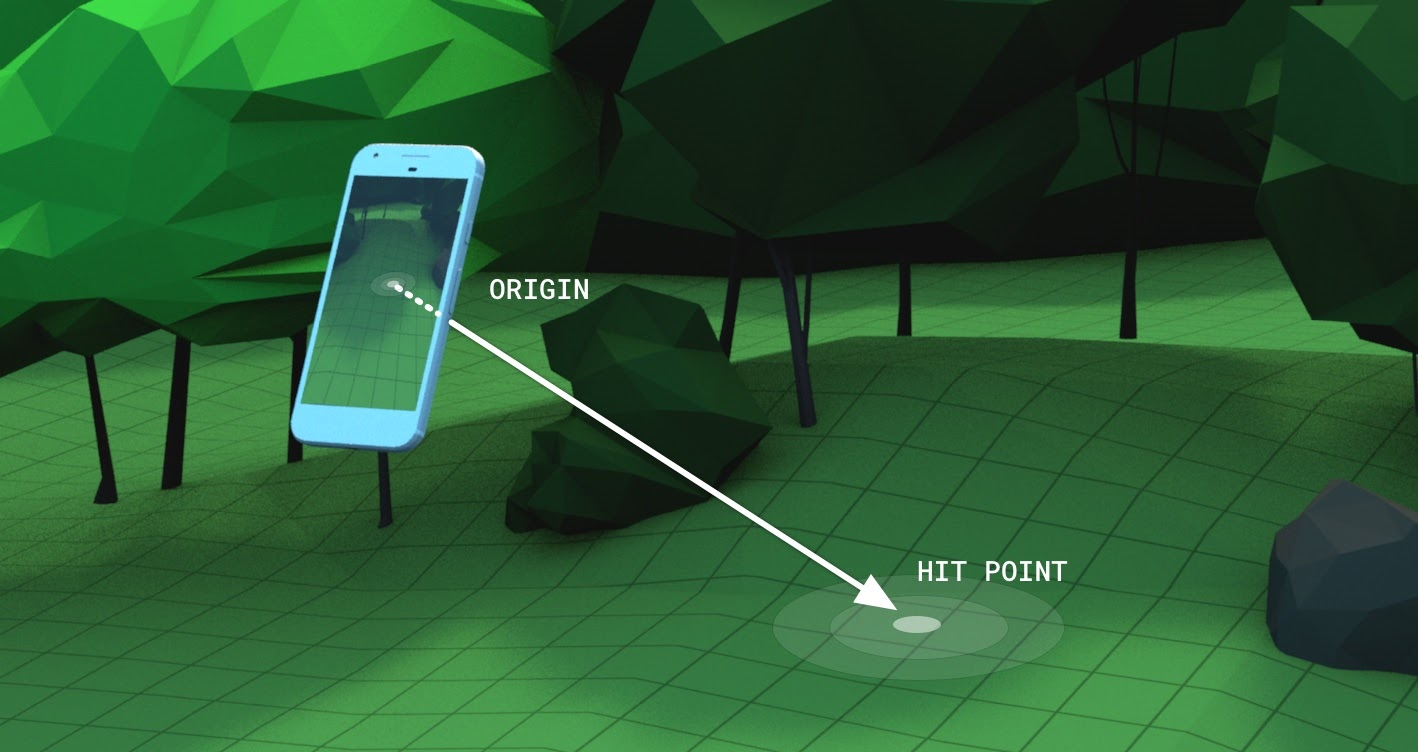
\includegraphics[width=8cm]{img/anwendung/arcore/hit-test-explainer.jpeg}
    \caption[Der hit-testing Strahl vom Smartphone trifft auf eine virtuelle Fläche und gibt ein Hit Ergebnis zurück.]{Der hit-testing Strahl vom Smartphone trifft auf eine virtuelle Fläche und gibt ein Hit Ergebnis zurück.\protect\footnotemark}
    \label{fig:anwendung-arcore-hit-test}
\end{figure}
\footnotetext{Quelle Bild: https://developers.google.com/ar/develop/hit-test, zuletzt aufgerufen am 09.08.2022}

In dieser Anwendung wird hit-testing dafür verwendet die Modelle auf den Flächen zu platzieren. Wird ein Hit zurückgegeben, wird dem Nutzer ein Pfeil auf der jeweiligen Fläche angezeigt. Der Pfeil dient als \textit{Placement Indicator}. Es hilft dem Nutzer bei der Platzierung der Objekte. Tippt der Nutzer auf den Bildschirm, wird das Gebäude an der Position des Hits platziert. Außerdem wird das hit-testing dazu genutzt bereits platzierte Gebäude zu detektieren. Die Implementierung in dieser Anwendug wird in Kapitel \ref*{technische-umsetzung-platzierung-auf-einer-beliebigen-flaeche-controller} erläutert. 

\subsubsection{Depth API}
\label{technische-umsetzung-arcore-depth-api}
Die Depth API generiert Tiefenbilder (\textit{depth maps}) um Tiefeninformationen der Umgebung zu erhalten. Es basiert auf der Arbeit von Flynn et al.\cite*{flynn2019}. Mit den Tiefenbildern werden die Position und die Größe von Objekten besser erkannt. Dies wird z.B. dafür genutzt, um \textit{Verdeckung (engl. Occlusion)} umzusetzen. Occlusion wird dann eingesetzt, wenn reale Objekte, die Näher am Betrachter liegen, das virtuelle Objekt verdecken. Wie in Abbildung \ref*{fig:anwendung-arcore-depth-api-occlusion} zu sehen wird die Katze vom realen Objekt verdeckt. Die Glaubwürdigkeit, dass eine echte Katze im Bild ist, steigt.

\begin{figure}[h]
    \centering
    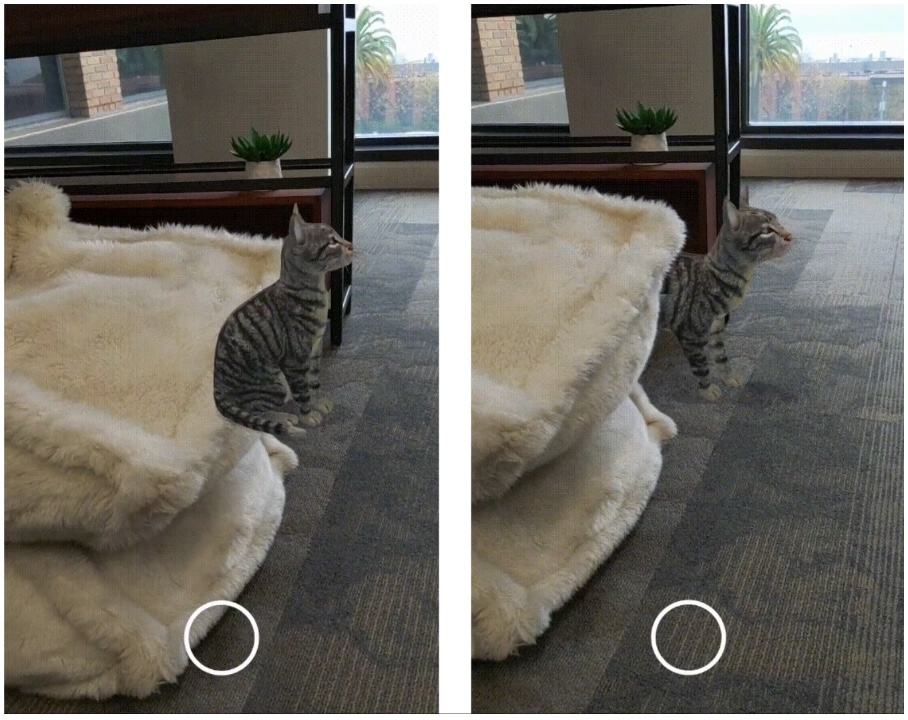
\includegraphics[width=8cm]{img/anwendung/arcore/arcore-depth-api-occlusion.jpg}
    \caption[AR ohne Occlusion (l.) und mit Occlusion (r.). Die virtuelle Katze wird durch das Objekt verdeckt.]{AR ohne Occlusion (l.) und mit Occlusion (r.). Die virtuelle Katze wird durch das Objekt verdeckt.\protect\footnotemark}
    \label{fig:anwendung-arcore-depth-api-occlusion}
\end{figure}
\footnotetext{Quelle Bild: https://developers.google.com/ar/develop/depth, zuletzt aufgerufen am 13.08.2022}

ARCore bietet zwei Ausgabemöglichkeiten für das Tiefenbild:

\begin{itemize}
    \item Raw Depth API liefert ein Tiefenbild mit hoher Genauigkeit. Dabei kann es vorkommen, dass nicht alle Pixel im Bild auch ein Tiefenwert erhält. Zusätzlich wird ein Konfidenzbild erzeugt.
    \item Full Depth API liefert ein geglättetes Tiefenbild. Pixel, die keinen Tiefenwert haben, erhalten einen geschätzten Wert.
\end{itemize}

Ein Konfidenzbild gibt jedem Pixel mit einem Tiefenwert einen Konfidenzwert zwischen 0 und 1. Je höher dieser Wert, desto höher ist die Wahrscheinlichkeit, dass die Tiefeninformation korrekt ist. Im Konfidenzbild wird dies durch die Pixelhelligkeit dargestellt. Je heller der Pixel im Konfidenzbild ist, desto höher ist der Konfidenzwert. Diese Funktion ist nützlich, um mit einem Threshold ungenaue Tiefeninformation auszuschließen.

Die Occlusion der Depth API zeigt in dieser Anwendung Probleme. Diese werden in Kapitel \ref*{probleme-grenzen-depth-api} aufgezeigt. Für den Anwendungszweck dieser Arbeit wird Occlsuion nur zum Testen für Entwickler in die Anwendung implementiert, da Ungenauigkeiten und Artefakte die Nutzererfahrung negativ beeinflussen.
%Neu in AR Core: global-scale location based Geospatial API
% - Vuforia
% -- Features
% - Wikitude
% -- Features
% - AR Toolkit
% -- Features
% - Unity & AR Foundation
% - AR Core und AR Kit
% -- Features
% -- Vorteile und warum diese SDK?
% -- Aufbau einer Szene
% UML (Was ist UML, wofür?)

%

\section{Aufgabenstellung}
Die Aufgabe besteht darin die im vorhergegangenen Arbeiten entstandenen 3D Modelle des SABA Gebäudes, des Lyautley- und des Mangin-Geländes mithilfe einer AR Applikation zu visualisieren. Ziel ist es eine App zu entwickeln, die eine hohe Immersion bietet. Daher wird zunächst der Begriff der Immersion in AR-Anwendungen definiert. Die Zielgruppe sind Bewohner der Stadt Villingen und interessierte Personen wie Touristen, die mehr über die Geschichte der Stadt Villingen erfahren möchten. Die Anwendung wird vor Ort genutzt, da die Geäude im Größenverhältnis 1:1 dargestellt werden. So hat der Nutzer ein direktes Verständnis über die Größenverhältnisse der Gebäude. Die 3D Modelle sollen an das Umgebungslicht und der herrschenden Wetterbedingungen angepasst sein. Das bedeutet, dass bei harten Licht die Modelle auch harte Schattenkanten werfen. Bei regnerischen Wetter soll die Fassade dunkler wirken, diffuse Schatten werfen und eventuell Spiegelungen darstellen.

\subsection{Fragestellungen / Problemstellungen}
Was sind die Probleme in der Entwicklung von AR Anwendungen im Freien?

- GPS ungenauigkeit

- größere Entfernung -> genaueres Tracking benötigt

Realistisches Umgebungsslicht

Wetterphänome und Darstellung in Computergraphik

\section{Forschungsstand}
\subsection{Ähnliche Arbeiten}
Outdoor AR Projekte

Wie wurden die Probleme gelöst?

\section{Tracking}
Definition, was ist mit dem Begriff gemeint?
\subsection{Koordinatensysteme}
\subsection{Kamera-basiertes Tracking}
\subsection{Marker Tracking}
\subsection{Marker-less Tracking}
\subsection{Algorithmen zur Erkennnung von Merkmalen}
\subsubsection{SIFT}
\subsubsection{SURF}
\subsubsection{ORB}
\subsubsection{Merkmalserkennung in AR Foundation / AR Core}
\subsection{SLAM}
Mathematische Definition des SLAM Problems und bekannte Arbeiten zur Lösung des Problems.
\subsection{SLAM in ARFoundation / AR Core}
\subsection{GPS Tracking}


\section{Computergraphik Shader}
Darstellung von Wetterphänomenen (hartes/diffuses Licht, Spiegelungen, Raytracing?)
- Raytracing in mobiltelefon in Unity machbar?
\subsection{Rendering Pipeline}
\subsection{Darstellung von Wetterphanomenen in der Computergraphik}
\subsection{Erkennung der Lichtsituation in AR Foundation / AR Core}
\subsection{Spiegelungen, Raytracing(?)}
Wie werden Spiegelungen erzeugt?

Raytracing, auch in Smartphones schon möglich?

\section{Entwicklung}
\subsection{Methodiken in der Planung}
UML, Agile Softwareentwicklung

\subsection{Frameworks}
\subsection{(Vergleich vorhandener Frameworks)}
Was gibt es auf dem Markt (AR Foundation, AR Core, AR Kit, Vuforia, Kudan, Wiktude), Vorteile/Nachteile und geeignetes Framework für die Entwicklung dieser App.
\subsection{Entwicklungsumgebung}
Ein paar beschreibende Worte über AR Foundation und Unity.

Welche Sprache wird genutzt?

Wie erfolgt die Entwicklung? Code schreiben, Debugging, Smartphone anschließen

Was muss für die Entwicklung installiert werden?

\subsection{Aufbau der Anwendung}
Beschreibung des Aufbaus der App, also die UML Grafik

\section{Nutzertest bzw. Evaluierung}
\subsection{Aufbau des Tests}
\subsection{Durchführung}
\subsection{Ergebnisse/Evaluierung}

\section{Fazit der Arbeit}
\section{Ausblick}
\subsection{Umsetzung der Anwendung}
\label{technische-umsetzung-umsetzung-der-anwendung}
Dieser Abschnitt erläutert den Aufbau der Szenen in Unity, um einen Überblick der erforderlichen Komponenten zu erhalten. Zunächst wird darauf eingegengen, wie eine Szene in AR Foundation aufgebaut ist. Dann wird ein Überblick über die verwendeten Skripte und deren Funktion in der Anwendung geschaffen, damit sich interessierte Entwickler schnell zurecht finden. 

Im Anschluss wird die Anbindung mit der REST-API erklärt. Die Antwort der API und die damit erzeugten Effekte werden aufgezeigt.

\subsubsection{Grundaufbau der AR Szenen in Unity}
\label{technische-umsetzung-platzierung-auf-einer-beliebigen-flaeche}
% Was wird gebraucht?
% Szenenaufbau
Bei der Erstellung eines neuen Projekts in Unity kann ein Standard Template für die Entwicklung von AR ausgewählt werden. Dieses beinhaltet Beispielszenen, Assets und die benötigten Packages. Diese können in normalen Unity Projekten im Package Manager installiert werden. Die benötigten Packages sind wie in Abbildung \ref*{fig:anwendung-umsetzung-packages} zu sehen in einem Gesamtpaket für AR vorhanden.

\begin{figure}[H]
    \centering
    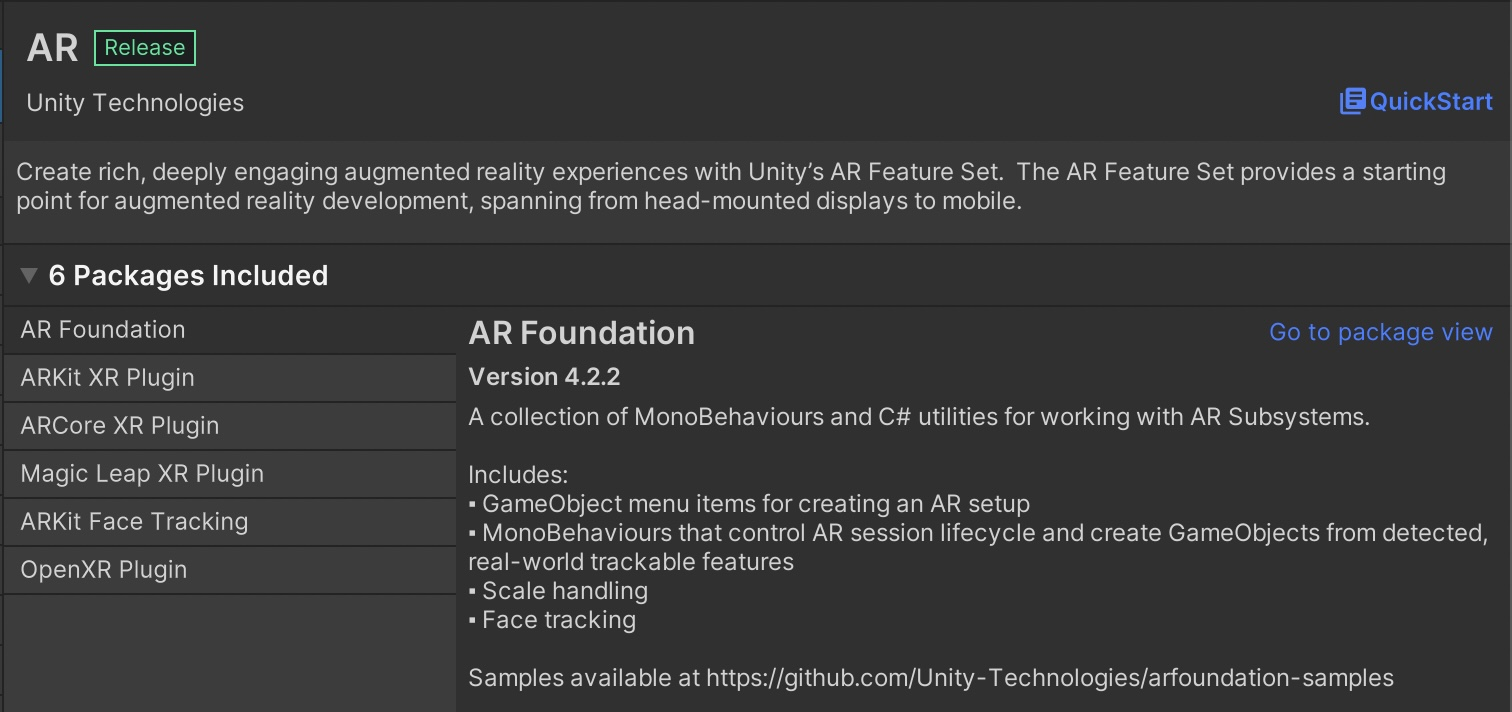
\includegraphics[width=8cm]{img/anwendung/technisch/ar-setup/setup-ar-unity.jpg}
    \caption{Die benötigten Packages im Package Manager.}
    \label{fig:anwendung-umsetzung-packages}
\end{figure}

Damit ARCore Zugriff auf die Packages hat, muss in den Projekteinstellungen unter \textit{XR Plug-in Management} Einstellungen vorgenommen werden. Unter dem Tab für Android muss ARCore als Plug-in Provider aktiviert werden. Damit wird das Plug-In für ARCore aktiviert und es kann auf die Kamera des Smartphones zurückgegriffen werden.

Eine einfache AR Szene besteht aus drei wichtigen Szenenobjekten, die in Abbildung \ref*{fig:anwendung-umsetzung-szenenaufbau} zu sehen sind: die \textit{AR Session}, die \textit{AR Session Origin} und die \textit{AR Camera}.

\begin{figure}[H]
    \centering
    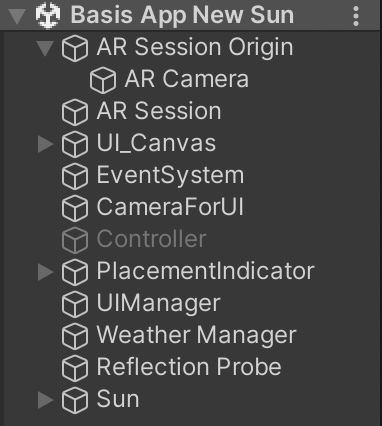
\includegraphics[width=5cm]{img/anwendung/technisch/ar-setup/setup-szenenaufbau.jpg}
    \caption{Der Szenenaufbau für die Position auf beliebigen Flächen.}
    \label{fig:anwendung-umsetzung-szenenaufbau}
\end{figure}

Die \textit{AR Session} ist ein \textit{GameObject}, dass das AR Session Skript enthält. Dieses sorgt für das Tracking. Wird das AR Session Skript deaktiviert, werden keine Schlüsselpunkte mehr erzeugt. Wird das Skript wieder aktivert, wird versucht die bestehenden Schlüsselpunkte weiterhin zu nutzen.

\begin{figure}[H]
    \centering
    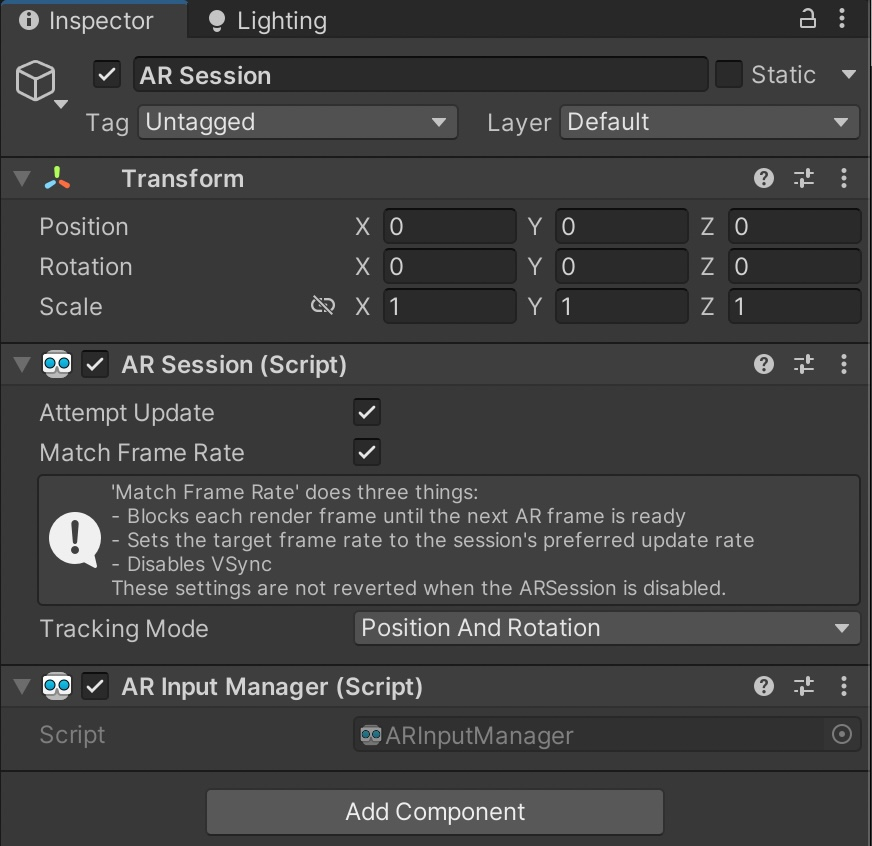
\includegraphics[width=6cm]{img/anwendung/technisch/ar-setup/setup-arsession.jpg}
    \caption{Die AR Session.}
    \label{fig:anwendung-umsetzung-arsession}
\end{figure}

Die \textit{AR Session Origin} ist auch ein \textit{GameObject}, an dem das AR Session Origin Skript hängt. Es transformiert die Trackable Objekte, wie z.B.  Schlüsselpunkte und Flächen, in ihre finale Position, Orientierung und Skalierung in das Weltkoordinatensystem von Unity. Die Skalierung der AR Session Origin bestimmt damit auch die Skalierung der Objekte in der Szene. Ist die Skalierung auf 0.1 gesetzt, so werden die Objekte in der Szene um den Faktor 0.1 verkleinert. Dies ist ein wichtiger Aspekt für die korrekte Skalierung der Gebäude, damit diese in der GPS Platzierung in der korrekten Größe dargestellt werden. Außerdem werden an der AR Session Origin die Skripte angehängt, die für einige ARCore Funktionen zuständig sind. So hängt für diese Anwendung der AR Plane Manager und der AR Raycast Manger daran.

\begin{figure}[H]
    \centering
    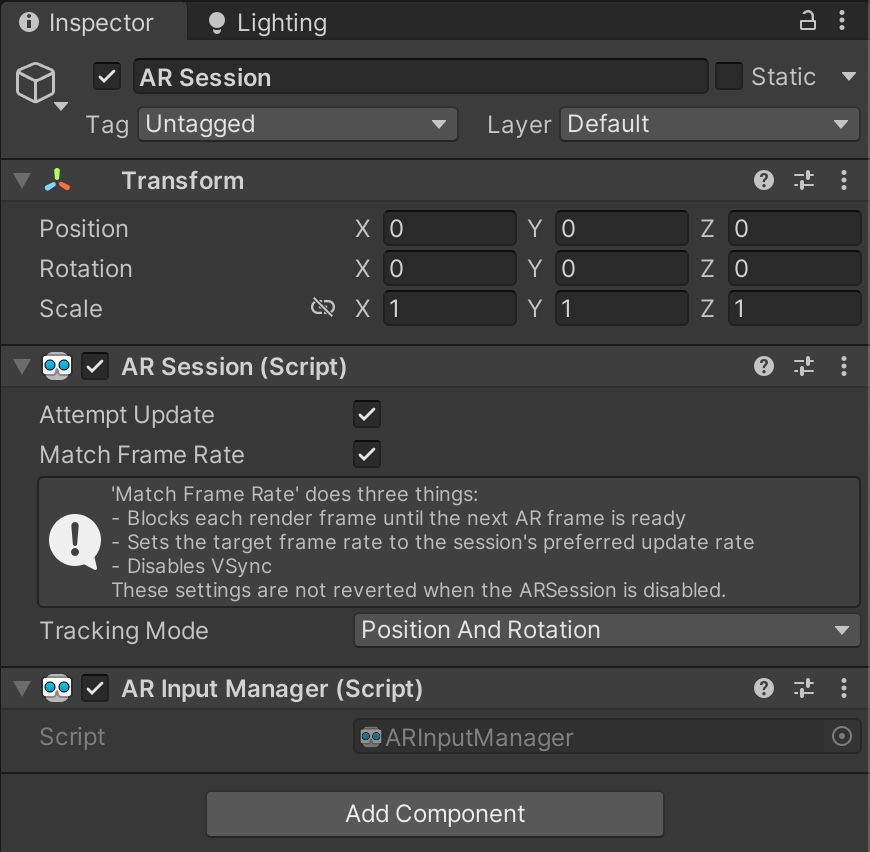
\includegraphics[width=6cm]{img/anwendung/technisch/ar-setup/setup-arsessionorigin.jpg}
    \caption{Die AR Session Origin mit dem AR Plane Manager und dem AR Raycast Manager.}
    \label{fig:anwendung-umsetzung-arsessionorigin}
\end{figure}

Das dritte Szenenobjekt ist die \textit{AR Camera}. Dies ist die Kamera von Unity mit zusätzlichen Komponenten. Diese sind der \textit{AR Camera Manager}, der \textit{AR Camera Background} und der \textit{Tracked Pose Driver}. Im AR Camera Manager wird die Light estimation und dessen Modus aktiviert. Die \textit{Facing Direction} bestimmt, ob die Front- oder die Rückkamera des Smartphones genutzt wird. Das AR Camera Background Skript sorgt dafür, dass das Kamerabild des Smartphone als Hintergrund angezeigt wird. Im Tracked Pose Driver werden Einstellungen vorgenommen, die für die Bestimmung der Position und Orientierung benötigt werden. Im Falle von AR im Smartphone wird hier festgelegt, dass die Pose über die Kamera berechnet wird. Die AR Camera wird als Kindelement der AR Session Origin eingefügt.

\begin{figure}[H]
    \centering
    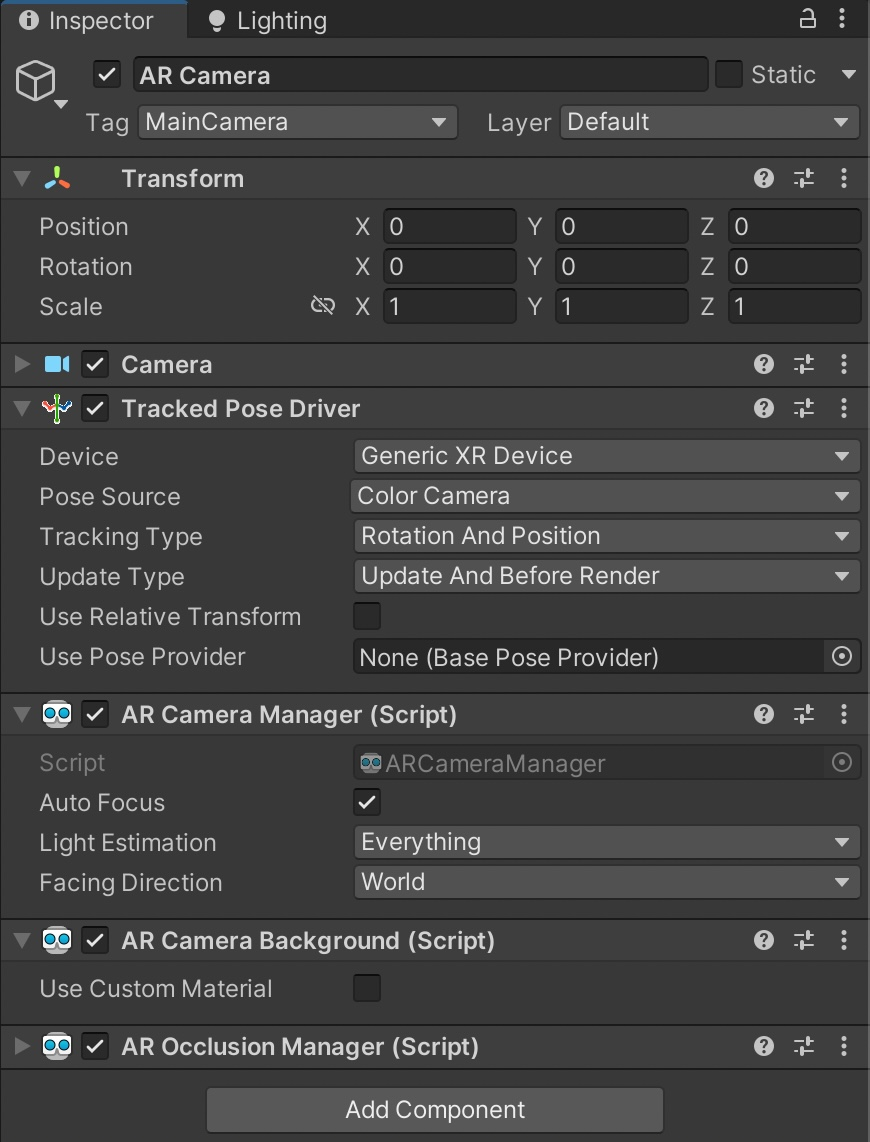
\includegraphics[width=6cm]{img/anwendung/technisch/ar-setup/setup-arcamera.jpg}
    \caption{Die AR Camera. Der Occlusion Manager aus der Depth API wird hier als Komponente eingefügt.}
    \label{fig:anwendung-umsetzung-arcamera}
\end{figure}

Diese drei Elemente werden für jede AR Anwendung in AR Foundation benötigt. Ausführliche Erklärungen zu den einzelnen Komponenten sind in der AR Foundation Dokumentation zu finden \cite*{UnityARFoundation}.

\subsubsection{Controller}
\label{technische-umsetzung-platzierung-auf-einer-beliebigen-flaeche-controller}
Der \textit{Controller} in der Szene aus Abbildung \ref*{fig:anwendung-umsetzung-szenenaufbau} ist ein \textit{GameObject}, das die Logik der Interaktionen beinhaltet. Alle Interaktionsmöglichkeiten (bis auf das User Interface) werden über dieses \textit{GameObject} geregelt. In den folgenden Abschnitt werden diese Funktionen kurz erläutert, damit ein Überblick über die verwendeten Skripte geschaffen wird.

\subsubsubsection{Platzieren auf einer beliebigen Fläche}
\label{technische-umsetzung-platzierung-normal}
Für die Platzierung der Gebäude ist das Skript \texttt{ARPlaceObjectAndMove.cs} zuständig. Wie in Kapitel \ref*{technische-umsetzung-arcore-user-interaction} erwähnt, wird in dieser Anwendung Raycast verwendet, um bei einem Hit einen Pfeil auf einer erkannten Ebene zu zeigen. Dieser dient als Placement Indicator. Wird eine Fläche erkannt, wird mit einem Tip auf dem Bildschirm das Gebäude platziert. Die Position und Orientierung wird vom letzten registrierten Hit bestimmt. Die Implementierung ist mit dem Code von Kris Schultz erfolgt\footnote{https://github.com/TheUnityWorkbench/tuw-arfoundation-demo/blob/master/Assets/Demo/ARTapToPlaceObject.cs, zuletzt aufgerufen am 13.08.2022}. Die Abbildung \ref*{fig:anwendung-umsetzung-platzierung} zeigt den Placemet Indicator und wie die das Gebäude platziert wird.

\begin{figure}[H]
    \centering
    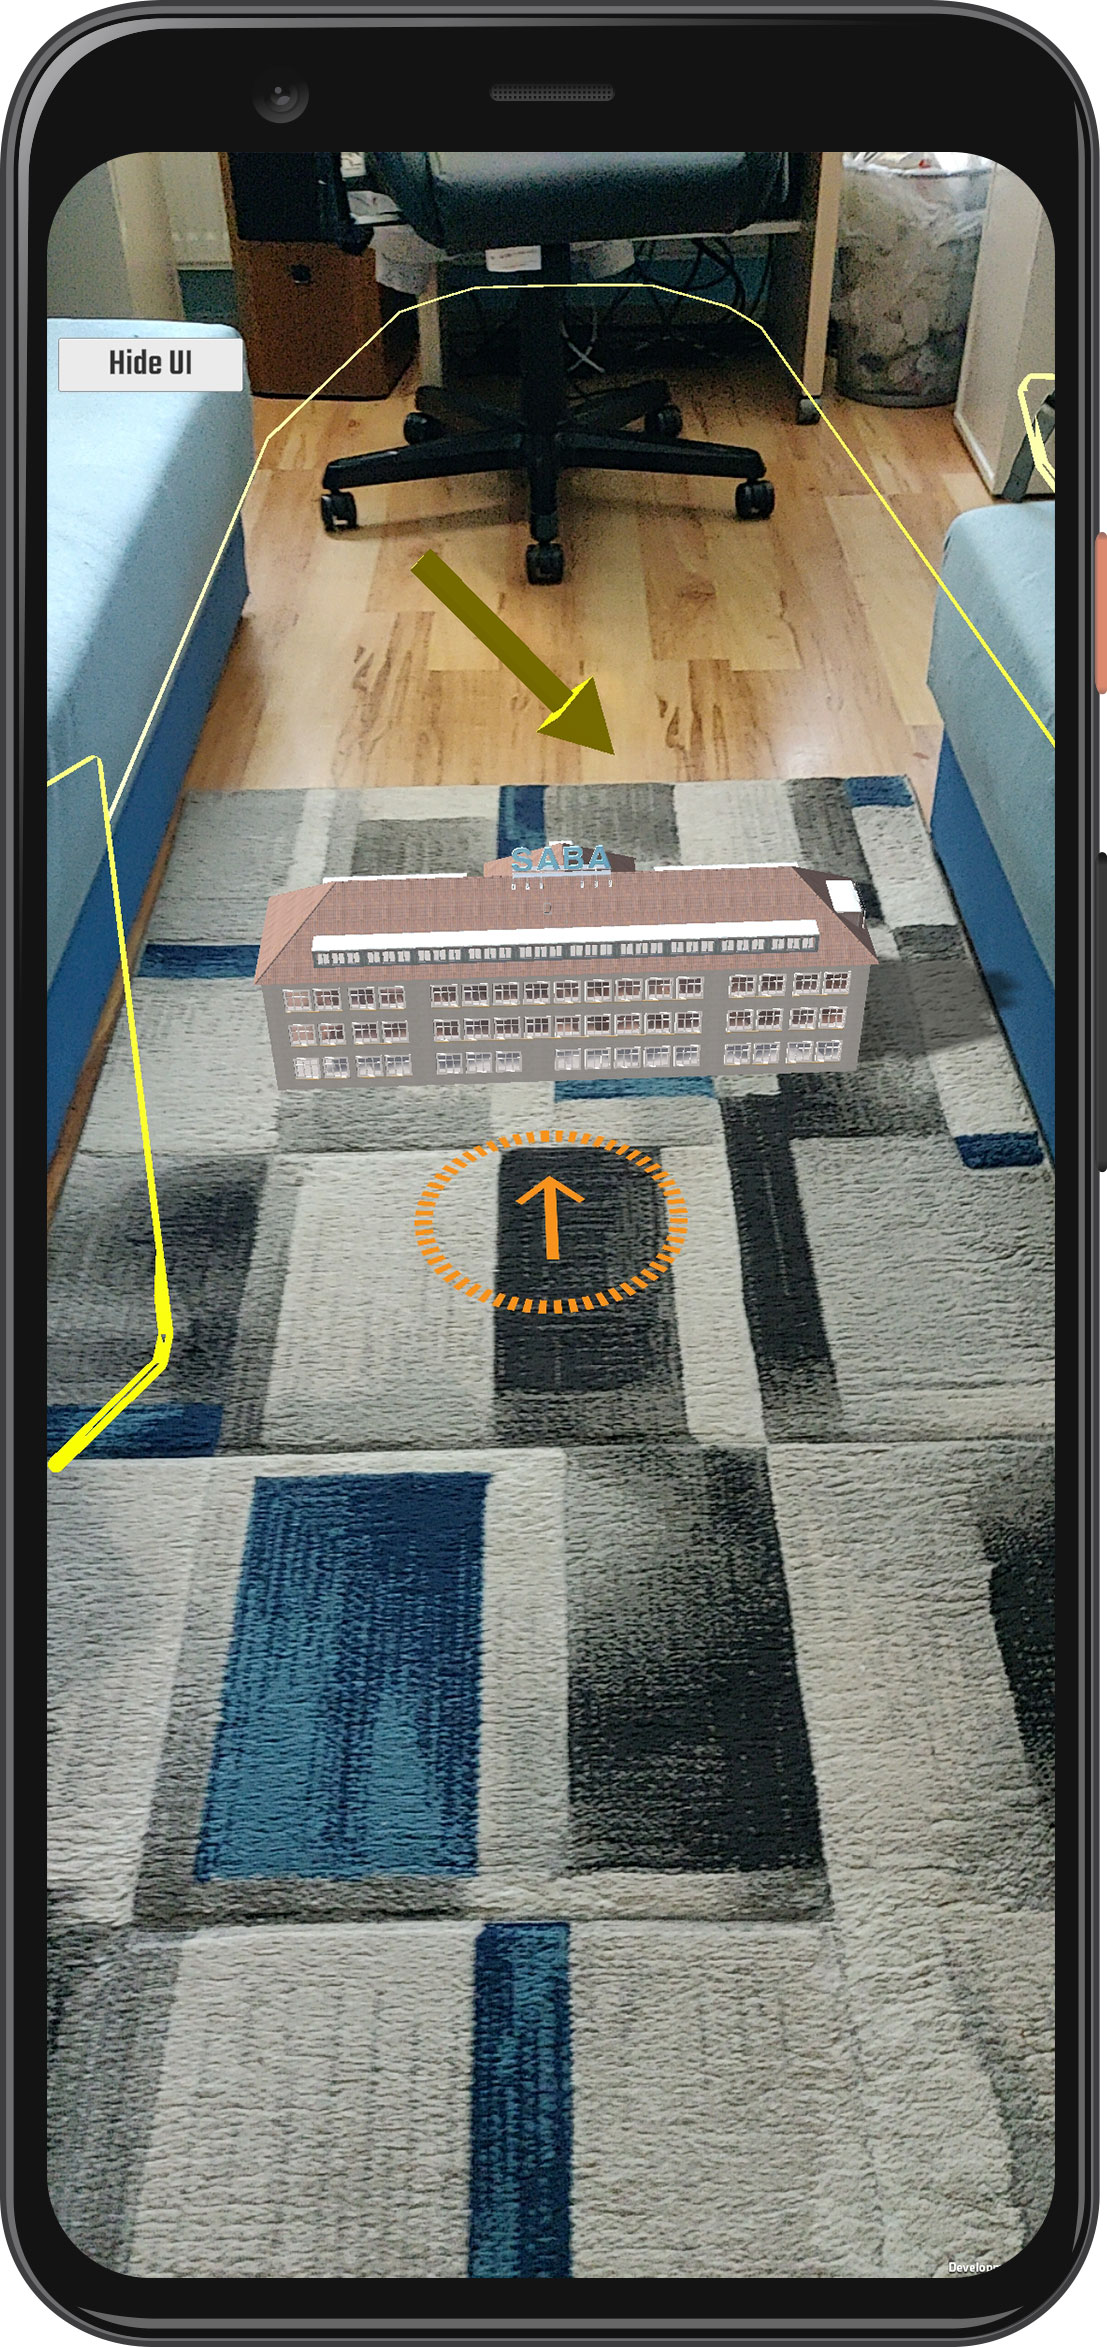
\includegraphics[width=6cm]{img/anwendung/technisch/controller/placement-indicator-beispiel.jpg}
    \caption{Der Pfeil auf dem Boden signalisiert, dass auf dieser Fläche Objekte platziert werden können.}
    \label{fig:anwendung-umsetzung-platzierung}
\end{figure}

Die Funktion \texttt{ARPlaceObject()}\footnote{unter Schultz als \texttt{PlaceObject()} benannt} wird für diese Anwendung modifiziert. Dies ist nötig, um die Funktion zu implementieren, dass das vom Nutzer ausgewählte Objekt platziert wird. Außerdem wird überprüft, ob es bereits eine Instanz des Gebäudes in der Szene gibt. Es soll nicht möglich sein ein Gebäude mehrmals zu platzieren.

Hierfür werden die aus Kapitel \ref*{konzept-der-anwendung} erwähnten BuildingGPS Scriptable Objects benötigt. Es werden zwei Listen geführt. Die Liste in Zeile 11 im unteren Code beinhaltet nur die Prefabs, die für die \texttt{Instantiate()} Funktion gebraucht wird. Die zweite Liste in Zeile 19 wird geführt, um das Scriptable Object des ausgwählten Gebäudes zu speichern. Tippt der Nutzer nach der Platzierung nochmal auf den Bildschirm, wird die ID des ausgewählten mit den ID's aus der Liste verglichen. Stimmt eine ID überein, ist das ausgewählte Gebäude bereits in der Szene vorhanden. Die \texttt{ARPlaceObject()} Funktion wird nicht ausgeführt.

\begin{lstlisting}[language=C,caption={Die \texttt{ARPlaceObject()} Funktion.},captionpos=b,label=lst:arplaceobject-funktion]
public void ARPlaceObject()
{
    //Get the selected Object from the ObjectSelection Script. This Script is attached to the UIManager.
    choosedObject = selectionMenuScript.selectedObject;
    foreach (var currentBuilding in buildings)
    {
        //Check if there is an instance of the choosed building in the scene.
        if (currentBuilding.id == choosedObject.id)
        {
            //Add the object to a list.
            listOfSpawnedObjects.Add(
                Instantiate(
                    currentBuilding.prefab,
                    placementPose.position,
                    placementPose.rotation
                )
            );
            //add the object to the building info list, in order to check earlier, if the building already exists
            listOfSpawnedObjectsBuildingInfo.Add(choosedObject);
        }
    }
} // end function ARPlaceObject()
\end{lstlisting}

\paragraph*{Pinch Funktion zur Skalierung}
Neben der Platzierung der Gebäude wird im \texttt{ARPlaceObjectAndMove.cs} Skript ermöglicht, die Gebäude zu Skalieren und auf einer Fläche zu bewegen. Die Skalierung wird dann ausgeführt, wenn zwei Finger gleichzeitg den Bildschirm berühren. Die Distanz der beiden Finger während der Pinch Bewegung bilden den Wert für die Skalierung\footnote{Der verwendete Code: https://www.youtube.com/watch?v=ISBIu6Jzfk8, zuletzt aufgerufen am 13.08.2022}.

\paragraph*{Gebäudewahl und Positionsveränderung auf einer Fläche}
Die Bewegung auf einer Fläche wird mit einem Raycast implementiert. Dabei wird ein Strahl von der Position des Touches erzeugt. Das Gebäude wird an die Position verschoben, bei der der Strahl die Fläche geschnitten hat. Der verwendete Code ist aus dem Github Repository von Dilmer Valecillos\footnote{https://github.com/dilmerv/UnityARFoundationEssentials/blob/master/Assets/Scripts/PlacementWithDraggingDroppingController.cs, zuletzt aufgerufen am 13.08.2022}.

\subsubsubsection{Objekte auswählen}
Für das auswählen der Objekte im \texttt{SelectObject()} Skript wird wieder ein Raycast genutzt. Von der Position der Mitte des Bildschirms wird ein Strahl geschickt. Wird ein Hit registriert, so wird zunächst überprüft, ob das Objekt ein Gebäude ist. Zur Identifikation werden \textit{Tags} genutzt. Unity bietet die Möglichkeit jedem GameObject einen Tag zu geben. Ein Tag ist ein String, dass als Referenz für das GameObject genutzt werden kann\footnote{https://docs.unity3d.com/Manual/Tags.html, zuletzt aufgerufen am 15.08.2022}. Wie in Abbildung \ref*{fig:anwendung-umsetzung-tags} zu sehen, bietet Unity vorgefertigte Tags. Es können auch eigene Tags definiert werden, wie in diesem Anwendungsfall der \textit{Selectable} Tag. Wird ein Gebäude identifiziert, erhält das Gebäude einen Outline Shader. Dieser fügt dem Gebäude eine Umrandung hinzu, die dem Nutzer signalisiert, dass das Gebäude ausgewählt werden kann. Mit den Button \textit{Select} und \textit{Deselect} kann der Nutzer die Gebäude auswählen und anschließend verschieben, rotieren, skalieren und entfernen.

\begin{figure}[H]
    \centering
    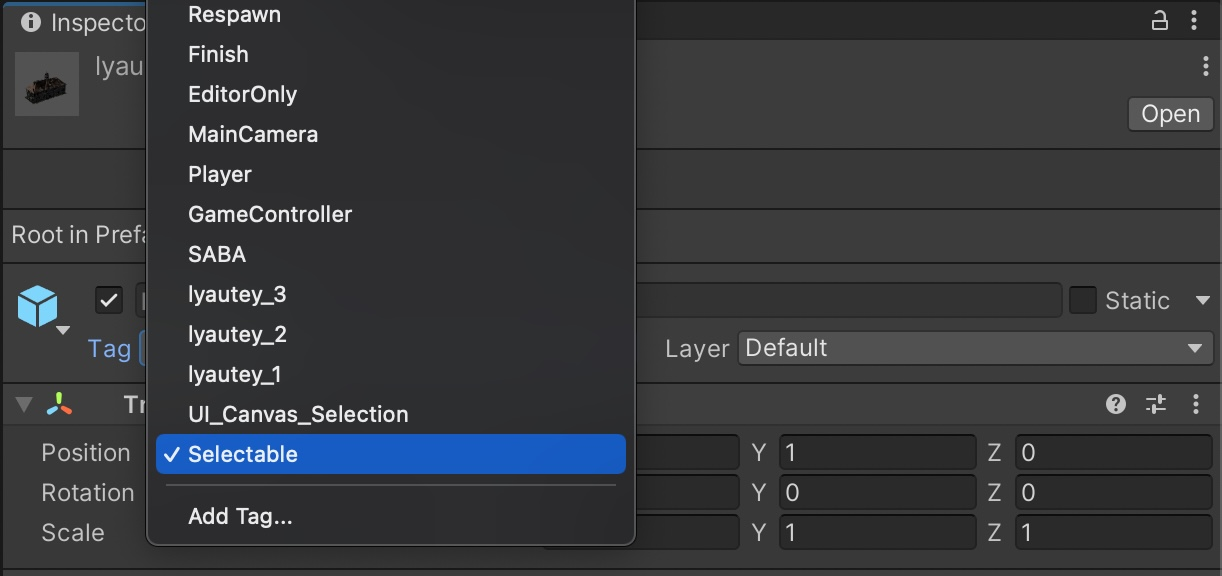
\includegraphics[width=8cm]{img/anwendung/technisch/controller/umsetzung-tags.jpg}
    \caption{Die Tag-Auswahl im Unity Inspector.}
    \label{fig:anwendung-umsetzung-tags}
\end{figure}

\paragraph*{Gebäude entfernen}
Zur Entfernung der Gebäude ist das Skript \texttt{DestroyObject.cs} zuständig. Mit dem Löschen Button wird die Funktion gestartet. Damit der Nutzer nicht aus versehen Gebäude löscht, wird ein Gebäude erst dann entfernt, wenn der Button für zwei Sekunden gedrückt wird. Es werden die zwei Listen aus dem \texttt{ARPlaceObjectAndMove.cs} Skript bearbeitet. Mit dem Befehl \texttt{Remove()} wird das jeweilige Gebäude aus den Listen entfernt und die Instanz des Gebäudes wird mit \texttt{Destroy()} zerstört.

\subsubsection{GPS Platzierung}
% Nativ nicht von AR Foundation. ARLocation aus dem Asset store
% Szenenaufbau, was wird gebraucht?
% UI
\label{technische-umsetzung-platzierung-gps}
Die Platzierung von Objekten über die GPS Informationen des Smartphones und der Angabe von GPS Längen- und Breitengraden ist nativ nicht mit AR Foundation möglich. Es können zwar GPS Informationen des Smartphones mit dem \textit{LocationService}\footnote{https://docs.unity3d.com/ScriptReference/LocationService.html, zuletzt aufgerufen am 15.08.2022} von Unity abgerufen werden. Das Platzieren von Objekten über GPS Koordinaten muss selbst implementiert werden. Hierfür wird das Asset \textit{AR + GPS Location} aus dem Asset Store benutzt\footnote{https://assetstore.unity.com/packages/tools/integration/ar-gps-location-134882, zuletzt aufgerufen am 15.08.2022}. Dieses Asset hat eine umfangreiche Dokumentation\footnote{https://docs.unity-ar-gps-location.com/, zuletzt aufgerufen am 15.08.2022}. Für das Asset werden weitere GameObjects in der Szene benötigt. In der \textit{AR Session Origin} wird ein \textit{AR Location Root} Objekt erzeugt. Außerdem wird in die Szene ein \textit{GPS Stage Object} gebraucht, das das \texttt{PlaceAtLocation.cs} Skript trägt. Dieses Objekt dient als Parent für jedes Objekt, das in der Szene platziert werden soll. Die jeweiligen GPS Koordinaten können im Inspector eingetragen werden. 

Da der Nutzer keine Auswahl hat, welches Gebäude platziert wird, wird jedes Gebäude aus der hinterlegten Datenbank platziert. Voraussetzung ist, dass das Gebäude innerhalb der eingestellten Render Distanz von Unity liegt. Ansonsten wird das in Kapitel \ref*{grp-geometrieverarbeitung-clipping} eingeführte Clipping durchgeführt und die Gebäude außerhalb des Einheitswürfels werden abgeschnitten. In dieser Anwendung ist die Render Distanz auf 250 Unity Einheiten gesetzt, was 250 Metern entspricht\footnote{https://docs.unity3d.com/ScriptReference/Camera-farClipPlane.html, zuletzt aufgerufen am 15.08.2022}. Dies genügt, um drei Gebäude nebeneinader zu platzieren. So ist es vor Ort mit den Gebäuden 2, 3 und 4 der Fall ist. 

Für die GPS Platzierung wird das \texttt{ARPlaceObjectAndMove} Skript angepasst. Die \texttt{MoveObject()} Funktion wird nicht mehr benötigt. Der untere Code zeigt die Anpassungen an der \texttt{ARPlaceObject()} Funktion. Für jedes Gebäude wird zunächst eine \texttt{Location} erzeugt. Dies ist ein Scriptable Object vom Asset\footnote{https://docs.unity-ar-gps-location.com/guide/\#locationdata, zuletzt aufgerufen am 15.08.2022}. Hier werden die Längen-, Breiten- und Höhengrade eingetragen. Diese Angaben stammen aus der Datenbank der Gebäude. Der \texttt{AltitudeMode} bestimmt, ob der eingegebene Höhengrad verwendet werden soll, oder ob eine detektierte Fläche von ARCore für die Platzierung genutzt werden soll. Da die Höhengrade in der Regel nicht sehr genau sind, werden die erkannten Flächen von ARCore genutzt. Anschließend werden Optionen gesetzt, die für die Platzierung im nächsten Schritt benötigt werden. Mit der Funktion \texttt{CreatePlacedInstance()}, die vom Asset bereitgestellt wird, wird das jeweilige Gebäude platziert.

\begin{lstlisting}[language=C,caption={Die angepasste \texttt{ARPlaceObject()} Funktion für die Platzierung mit GPS.},captionpos=b,label=lst:GPS-arplaceobject-funktion]
void ARPlaceObject()
{
    foreach (var currentBuilding in buildings)
    {
        //set new location data
        var location = new Location()
        {
            Latitude = currentBuilding.latitude,
            Longitude = currentBuilding.longitude,
            Altitude = currentBuilding.altitude,
            AltitudeMode = AltitudeMode.GroundRelative
        };
        //set options
        var options = new PlaceAtLocation.PlaceAtOptions()
        {
            HideObjectUntilItIsPlaced = true,
            MaxNumberOfLocationUpdates = 2,
            MovementSmoothing = 0.1f,
            UseMovingAverage = false
        };
        //create Instance
        spawnedObject = PlaceAtLocation.CreatePlacedInstance(
            currentBuilding.prefab,
            location,
            options,
            false
        );
        //set Rotation to fit real facing direction
        spawnedObject.transform.rotation = Quaternion.Euler(0, 0, 0);
        var currentHeading = locationProvider.CurrentHeading.heading;
        spawnedObject.transform.Rotate(
            0,
            (float)currentHeading - currentBuilding.realWorldOrientation,
            0,
            Space.World
        );
        listOfSpawnedObjects.Add(spawnedObject);
    }
}
\end{lstlisting}

\subsubsubsection{Ausrichtung der Szene nach Norden}
\label{umsetzung-gps-ausrichtung-nach-norden}
% Orientierung nach Norden
Wie in Kapitel \ref*{tracking-koordinatensysteme} erwähnt, wird beim Start einer Unity Szene die Richtung bestimmt, in die die z-Achse des Weltkoordinatensystems zeigen wird. In AR Foundation ist dies die Richtung, in die die Kamera des Smartphones zeigt. Damit die Gebäude in die richtige Richtung zeigen, müsste der Nutzer die Szene dann starten, wenn das Smartphone genau nach Norden zeigt. Es wird ein Skript gebraucht, um die Szene nach Norden auszurichten. 

Mit Unity wird auf den Kompass des Smartphones zugegriffen. Da der Kompass in Smartphones ungenau ist, wird ein Tiefpassfilter verwendet. Dieser berechnet den Durchschnitt der letzten 10 Kompasswerte, um grobe Ausreißer der schwankenden Kompasswerte zu ignorieren. Die Kompasswerte liegen zwischen 0° und 360°. Falls der Wert bei Nordkurs zwischen 359° bis 1° schwankt, kann es zu Diskontinuitäten kommen. Der Durchschnittswert liegt dann bei 180°. Um dies zu vermeiden wird wird der Tiefpassfilter mit Sinus und Kosinus berechnet. Dies ist im unteren Code in der Zeile 24 zu sehen. 

Mit den Button \textit{Reorient} kann der Nutzer die Szene neu ausrichten. Das Ausrichten wirkt sich sowohl in der GPS Anwendung auf die Rotation der Gebäude aus, als auch auf die Position der Sonne. Die Sonne wird in Kapitel \ref*{technische-umsetzung-licht} behandelt.

\begin{lstlisting}[language=C,caption={Der Tiefpassfilter im \texttt{ReorientToNorth.cs} Skript},captionpos=b,label=lst:tiefpassfilter]
public float CalculateAverage()
{
    int dataSize = data.Count;
    //use low pass filter to determine the average compass direction
    float average = (float)(180 / Math.PI) * (float)Math.Atan2(sumSin / dataSize, sumCos / dataSize);
    return average;
}
\end{lstlisting}

\paragraph*{Ausrichtung der Gebäude}
Wenn die Szene nach Norden ausgerichtet ist, zeigt das Prefab des Gebäudes in die Richtung, mit der das Gebäude aus Blender exportiert wird. Die z-Achse des lokale Koordinatensystems des SABA Gebäudes ist z.B. in Abbildung \ref*{fig:umsetzung-gps-rotation-saba}(a) zu sehen. Damit das SABA Gebäude in die korrekte Richtung zeigt, wird das Gebäude um 72.47° in der y-Achse gedreht. Dieser Wert wird mithilfe einer Karte des Vermessungsamts Villingen-Schwenningen berechnet. Dieser Wert wird mit der Karte vom Gelände berechnet.
% Problem: Kompass ungenau
% Tiefpassfilter

\begin{figure}[H]
    \centering
    \subfloat[][]{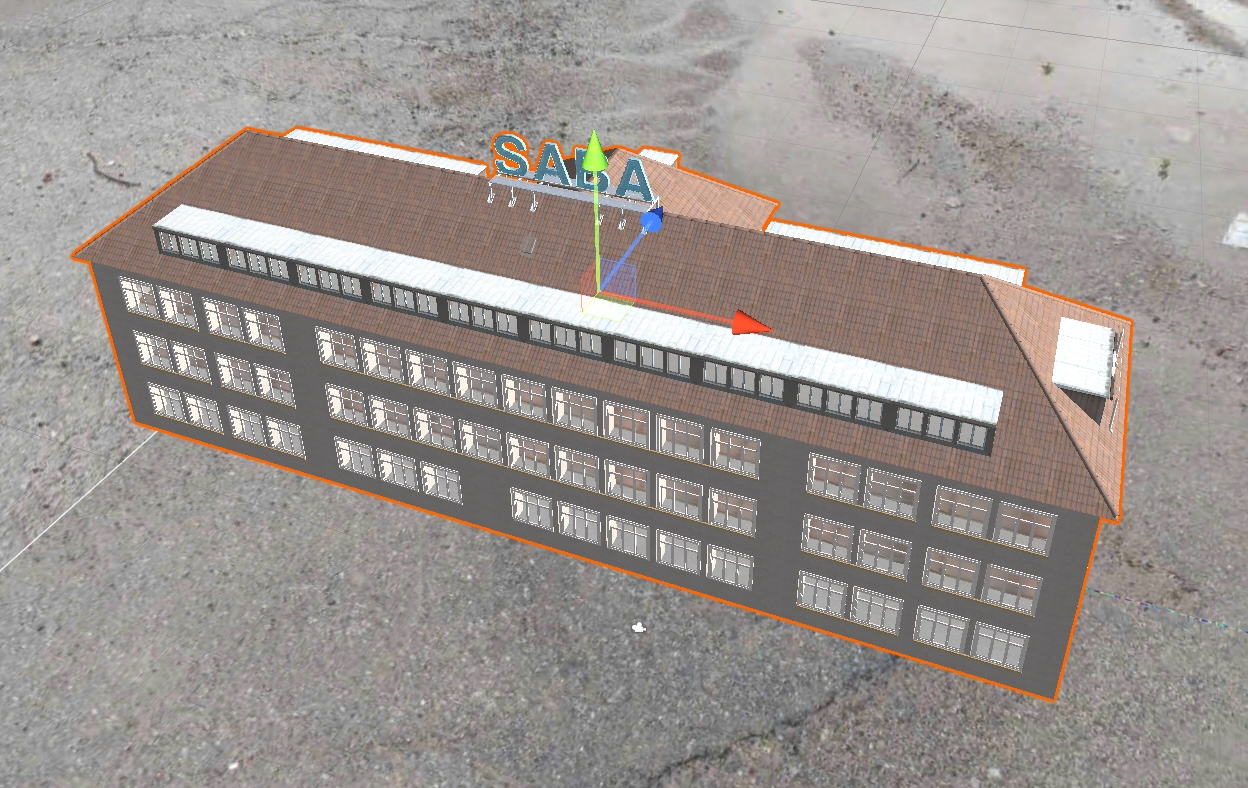
\includegraphics[width=0.5\linewidth]{img/anwendung/technisch/gps/konzeption-lokales-koordinatensystem-saba.jpg}}%
    \qquad
    \subfloat[][]{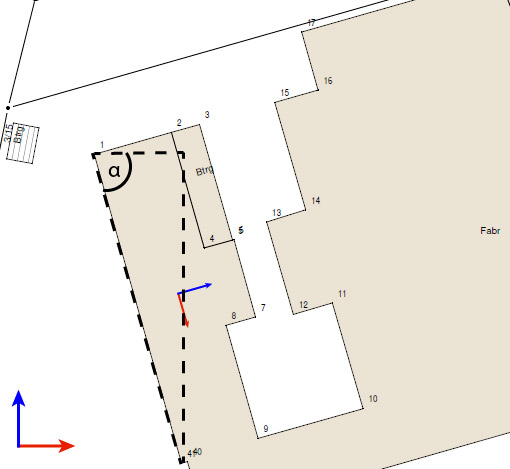
\includegraphics[width=0.4\linewidth]{img/anwendung/technisch/gps/SABA-winkel.jpg}}%
    \caption{Das lokale Koordinatensystem des SABA Gebäudes zeigt mit der z-Richtung (blauer Pfeil) nach Norden(a). Um den Winkel \textalpha  wird das Gebäude gedreht, damit die Rotation des Gebäudes mit den realen Gebäude übereinstimmt(b).}%
    \label{fig:umsetzung-gps-rotation-saba}
\end{figure}

Folgende Winkel werden für die Gebäude in dieser Anwendung verwendet:

\begin{table}[H]
    \centering
    \begin{tabular}{|p{0.25\textwidth}|p{0.04\textwidth}|p{0.4\textwidth}|p{0.15\textwidth}|}
    \hline
        Gebäude                 & Nr. &       lokales Koordinatensystem       & Winkel     \\ \hline 
        SABA                    & 1   & \parbox[c]{0.4\textwidth}{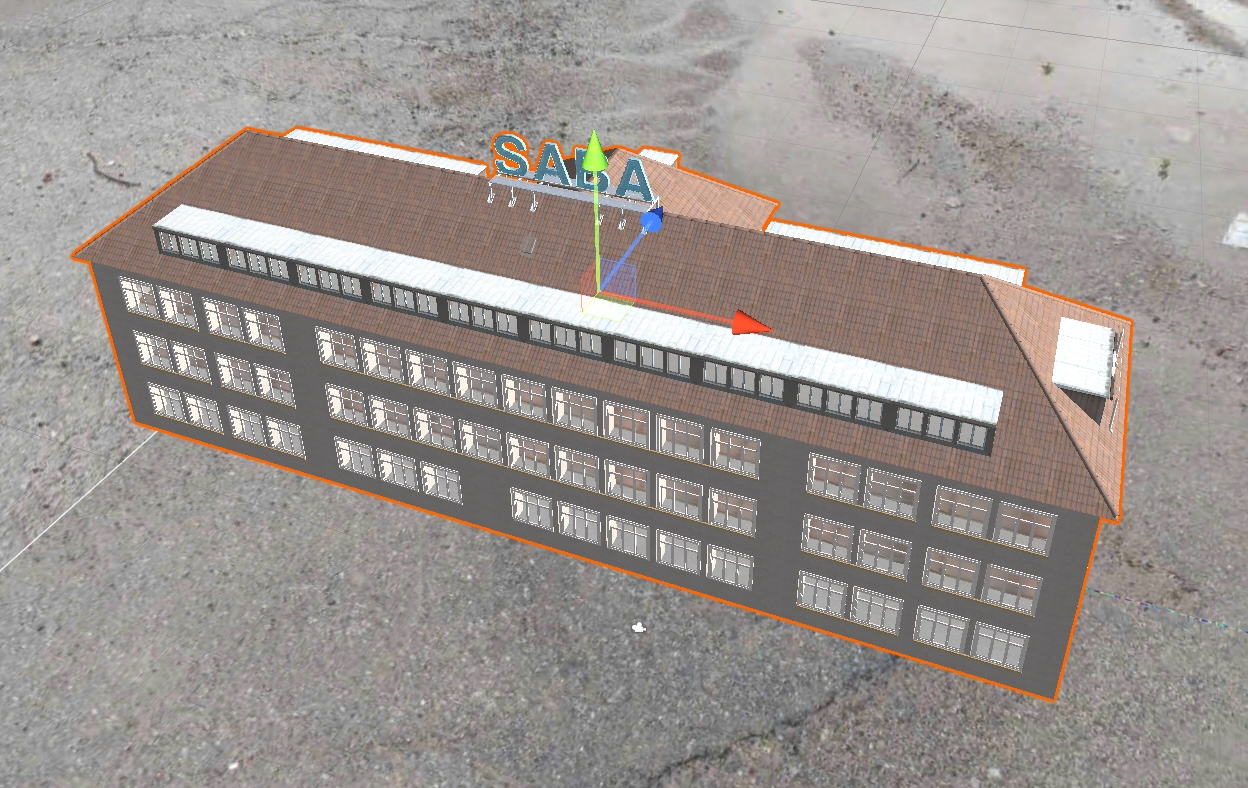
\includegraphics[width=0.4\textwidth]{img/anwendung/technisch/gps/konzeption-lokales-koordinatensystem-saba.jpg}} & 74,32°     \\ \hline
        Reithalle               & 2   & \parbox[c]{0.4\textwidth}{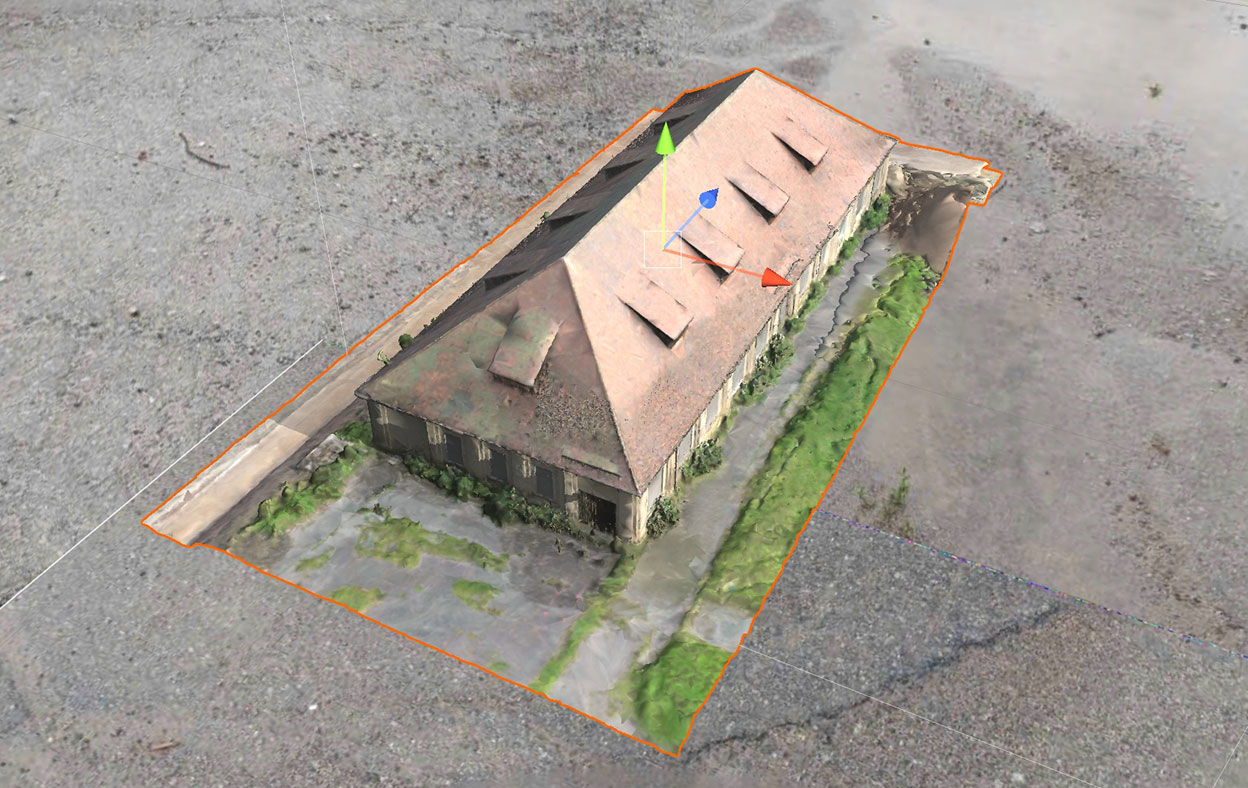
\includegraphics[width=0.4\textwidth]{img/anwendung/technisch/gps/konzeption-lokales-koordinatensystem-l1.jpg}}                                     & 33,54°  \\ \hline
        Mannschaftsgebäude 1    & 3   & \parbox[c]{0.4\textwidth}{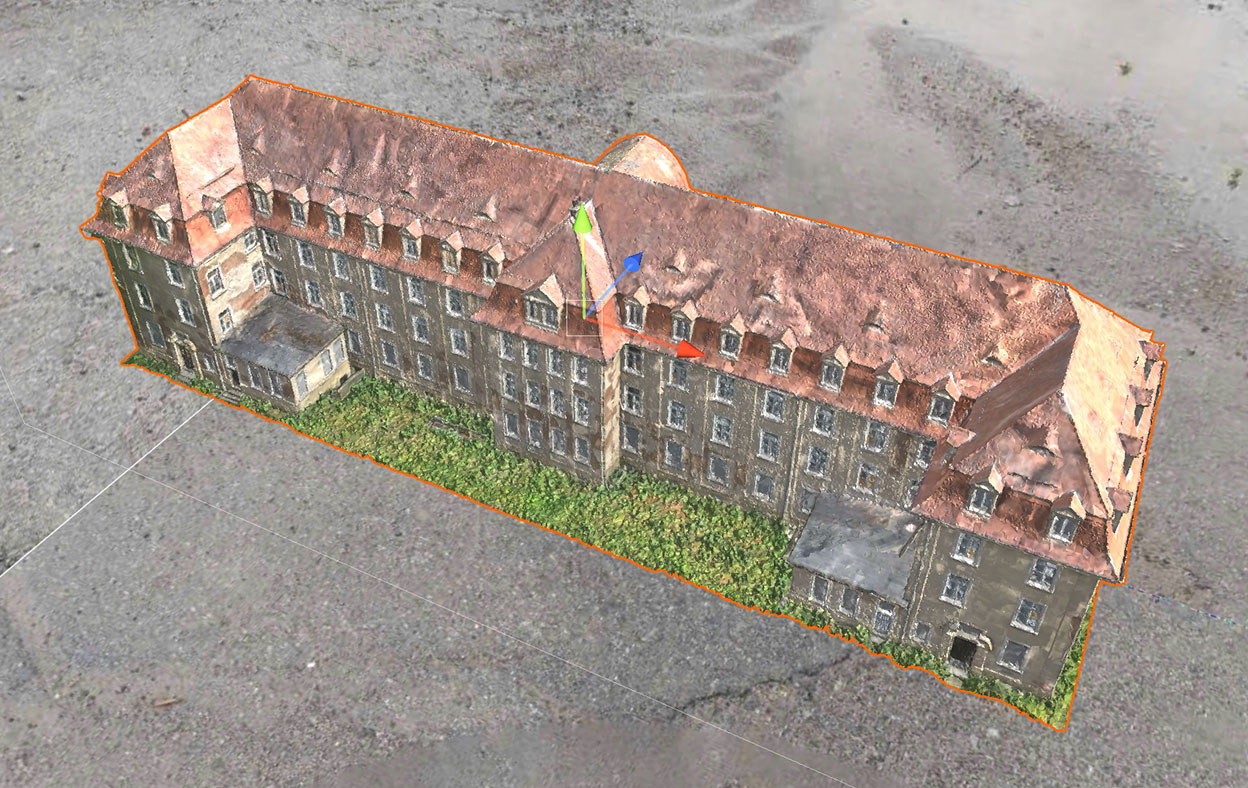
\includegraphics[width=0.4\textwidth]{img/anwendung/technisch/gps/konzeption-lokales-koordinatensystem-l2.jpg}}                                     & 208,00°     \\ \hline
        Wirtschaftsgebäude\footnotemark      & 4   & \parbox[c]{0.4\textwidth}{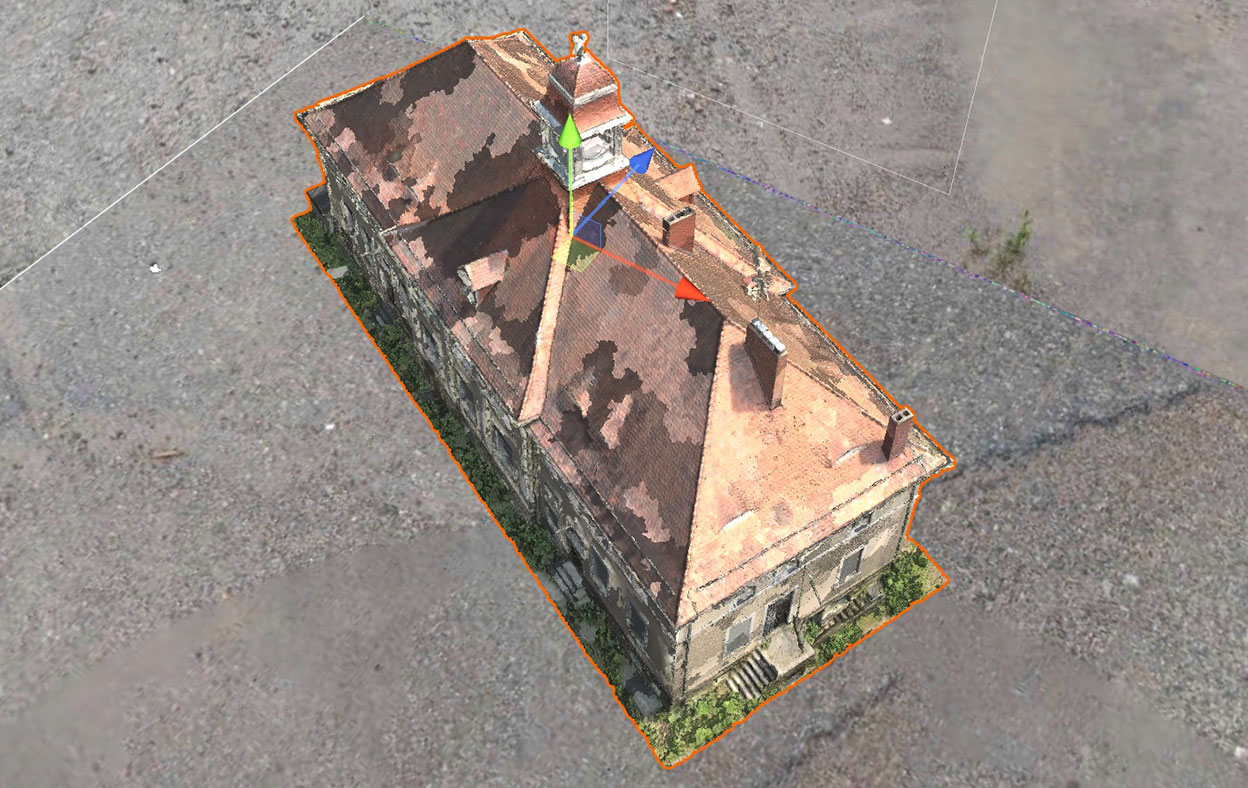
\includegraphics[width=0.4\textwidth]{img/anwendung/technisch/gps/konzeption-lokales-koordinatensystem-l3.jpg}}                                     & 23,10°     \\ \hline
        Mannschaftsgebäude 2    & 5   & \parbox[c]{0.4\textwidth}{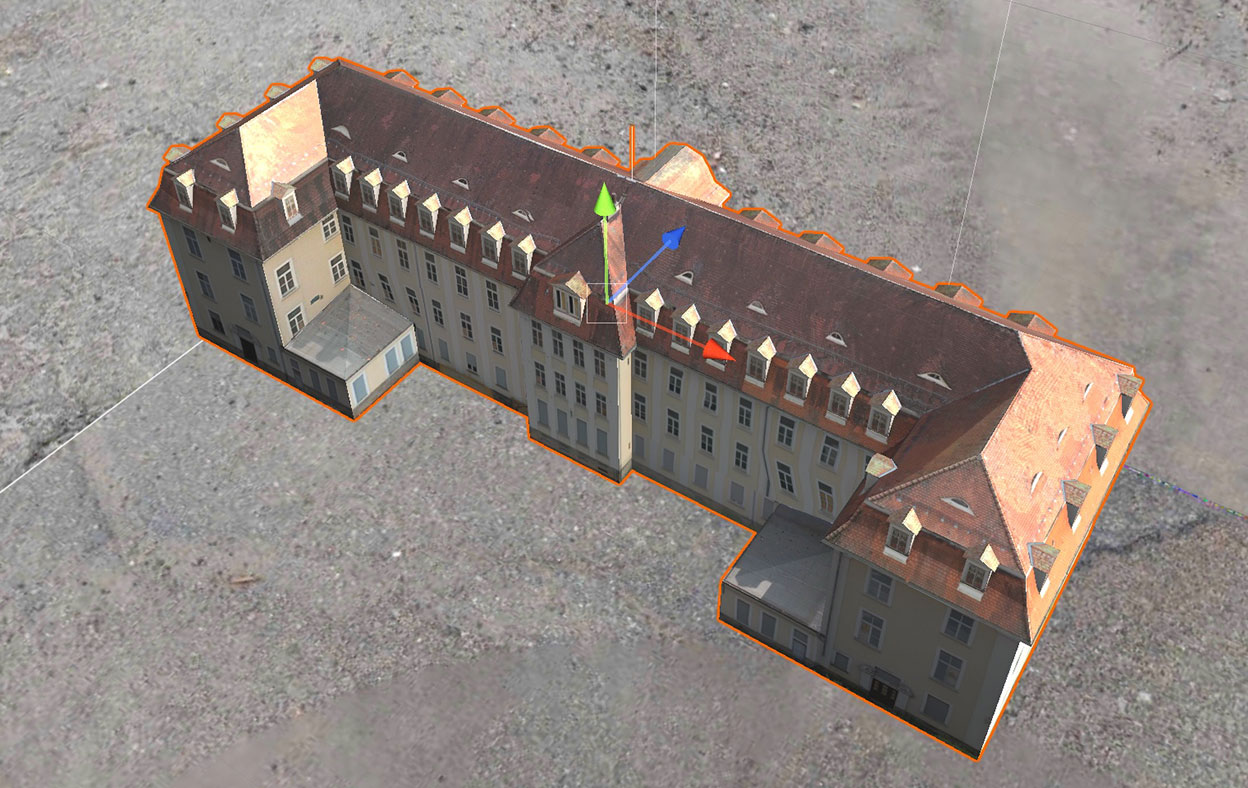
\includegraphics[width=0.4\textwidth]{img/anwendung/technisch/gps/konzeption-lokales-koordinatensystem-l4.jpg}}                                      & 20,40°       \\ \hline
    \end{tabular}
    \caption{Die lokalen Koordinatensysteme der Gebäude und deren Winkelangaben zur korrekten Rotation.}
    \label{tab:umsetzung-gps-berechnete-winkel}
\end{table}

\footnotetext{Wie am Bild in der Tabelle zu sehen, ist das Gebäude bereits um den Winkel rotiert.}

\subsection{Belichtung}
\label{technische-umsetzung-licht}
% Wie wird die Beleuchtung geregelt?
Die Belichtung der Szenen besteht aus drei Komponenten. Mit der Light Estimation API wird der \textit{Ambient Intensity Mode} genutzt, um die durchschnittliche Helligkeit und die durchschnittliche Farbetmperatur zu bestimmen. Mit diesen Werten wird das Hauptlicht gefärbt, um die realen Lichtbedingungen einwirken zu lassen. Das Hauptlicht ist ein direktionales Licht, das die gesamte virtuelle Szene aufhellt. Dieses Licht simuliert die Sonne. Letzlich werden HDR Panoramabilder des SABA Geländes angefertigt, um Cubemaps zu generieren und \textit{Environmental Lighting} zu ermöglichen. In den folgenden Abschnitten wird die Implementierung der verwendeten Techniken gezeigt. Vorher und Nachher Vergleiche zeigen die Unterschiede bei der Belichtung.

\subsubsection{Light Estimation in dieser Anwendung}
\label{technische-umsetzung-light-estimation}



\subsubsection{Sonne simulieren}
% Sonne Setup

\subsection{Wetterbedingungen}
\label{technische-umsetzung-wetterbedingungen}
Dieses Kapitel behandelt die Umsetzung der Veränderungen an der Szene anhand von Wetterdaten. Zunächst wird die auf die Anbindung an die Wetter REST-API in Unity eingegangen. Danach wird veranschaulicht, welche Parameter angepasst werden. Ein anschließender Vergleich der einzelnen Wetterbedingungen zeigt die Auswirkungen auf die Optik der Gebäude. 

\subsubsection{Anbindung der REST-API}
Um Wetterdaten in \textit{Open Weather Map} abzufragen, wird ein Account benötigt. Genutzt wird die \textit{Current Weather} API\footnote{https://openweathermap.org/current, zuletzt aufgerufen am 19.08.2022}. Nach der Anmeldung wird im Account ein API Key generiert, der später im Skript für die Anfrage benötigt wird. 

Die Antwort der API erfolgt über eine \acrfull{json} Datei. Es ist ein Datenformat, das zum Datenaustausch zwischen Anwendungen genutzt wird. JSON Daten liegen in einfach lesbare Textform bereit und ist Programmiersprachen unabhängig\footnote{https://de.wikipedia.org/wiki/JavaScript\_Object\_Notation, zuletzt aufgerufen am 19.08.2022}. Um die Daten der JSON Datei zu nutzen, wird ein JSON-Parser in Unity benötigt. In dieser Anwendung wird SimpleJSON\footnote{https://github.com/Bunny83/SimpleJSON, zuletzt aufgerufen am 19.08.2022} genutzt. Das Skript wird als Asset in das Unity Projekt eingefügt.

Das Wetter wird in der Szene vom \textit{Weather Manager} und dem \texttt{WeatherManager.cs} Skript geregelt. Zunächst wird in einer \textit{Coroutine} durchgeführt, um die Längen- und Breitengrade der aktuellen Position zu ermitteln. Mit einer \textit{Coroutine} werden in Unity Arbeitsschritte durchgeführt. Zum Beispiel wird für eine Funktion 1 das Ergebnis einer anderen Funktion 2 benötigt. Mit einer \textit{Coroutine} wird dafür gesorgt, dass die Funktion 2 ausgeführt wird und Funktion 1 erst dann ausgeführt wird, wenn Funktion 2 vollständig durchlaufen ist. In diesem Fall wird für die Anfrage der Daten die Längen- und Breitengrade benötigt. Erst wenn diese vorhanden sind, erfolgt eine Anfrage der Daten.



\begin{lstlisting}[language=C,caption={Die \texttt{ARPlaceObject()} Funktion.},captionpos=b,label=lst:arplaceobject-funktion]
private IEnumerator FetchWeatherDataFromApi(string latitude, string longitude)
    {
        string url = currentWeatherApi + "lat=" + latitude + "&lon=" + longitude + "&appid=" + apiKey + "&units=metric";
        UnityWebRequest fetchWeatherRequest = UnityWebRequest.Get(url);
        yield return fetchWeatherRequest.SendWebRequest();
        if (fetchWeatherRequest.isNetworkError || fetchWeatherRequest.isHttpError)
        {
            //Check and print error
            statusText.text = fetchWeatherRequest.error;
        }
        else
        {
            Debug.Log(fetchWeatherRequest.downloadHandler.text);
            var response = JSON.Parse(fetchWeatherRequest.downloadHandler.text);

            //set UI Text
            location.text = "Ort: " + response["name"];
            weatherIDText.text = "WetterID: " + response["weather"][0]["id"];
            mainWeather.text = "Wetter: " + response["weather"][0]["main"];
            description.text = "Beschriebung: " + response["weather"][0]["description"];
            temp.text = response["main"]["temp"] + " C";

            //fetch data for further functions
            weatherID = response["weather"][0]["id"];

            if (IsWeatherImpactEnabled.isOn)
            {
                ChooseWeatherCase(weatherID);
            }
        }
    }
\end{lstlisting}
    


\subsubsection{Veränderungen der Wetter Parameter}
% Welche Parameter gibt es?

\subsection{Verwendete Shader}
% Konzept
% User Interface
% Aufbau der Szenen
% - Menü
% - GPS
% - Standard App
% Implementierung von Features
% - Plane Tracking
% - Occlusion
% - Light Estimation
% Implementierung von Wetter
% - API OpenWeatherMap Anbindung
% - OpenWeatherMap Codes nutzen
% -- States des Wetters
% Lichtsetzung
% - Sonne simulieren
% -- Position der Sonne bestimmen
% -- Farbtemperatur anpassen
% Shader
% - Shatten werfer für den Boden
% - Outline Shader
% - Nass Shader

%KAPITEL 5 Probleme und Lösungen
\subsection{Probleme und Lösungen}
\subsubsection{Grenzen der Depth API und Occlusion}
\label{probleme-grenzen-depth-api}
Wie in Kapitel \ref{immersion} beschrieben trägt eine gute Verdeckung der virtuellen Objekte dazu bei, die Immersion in AR zu steigern\cite*[Breen et al. (1995)][]{breen1995}\cite*[Shah et al. (2012)][]{shah2012}. Umso wichtiger ist es, dass diese Funktion auch in dieser Anwendung gut funktioniert. Dabei gibt es drei Problematiken, die bei der Entwicklung in dieser Arbeit zum Vorschein kommen.

Das erste Problem ist, das diese API nicht für jedes Gerät verfügbar ist. Die Dokumentation von ARCore\cite*{ARCoreDokumentation} bietet eine Tabelle mit allen kompatiblen Geräten. Damit kann nicht sichergestellt werden, dass die Anwendung auf jedem Gerät gleich funktioniert. 

Ein weiteres Problem wird in Abbildung \ref*{fig:technische-umsetzung-arcore-depth-problem} deutlich. In diesem Beispiel wird Occlusion mit dem \textit{AR Occlusion Manager} implementiert, der an die \textit{AR Camera} angehängt wird. Die AR Camera wird in Kapitel \ref*{technische-umsetzung-platzierung-auf-einer-beliebigen-flaeche} erläutert. Das Beispiel ist vor Ort an einer Mauer vor dem Gebäude 4 aufgenommen. Das rote Quadrat ist die erzeugte Depth Map. Je dunkler die rote Farbe, desto näher ist das Objekt zur Kamera. Es wird deutlich, dass erst ab einer Entfernung von 1m überhaupt Tiefe erkannt wird. Aus einer Entfernung ab 1,5m wird keine Tiefe mehr erkannt. Dies ist insbesondere für AR im Freien problematisch. 

\begin{figure}[H]
    \centering
    \subfloat[][]{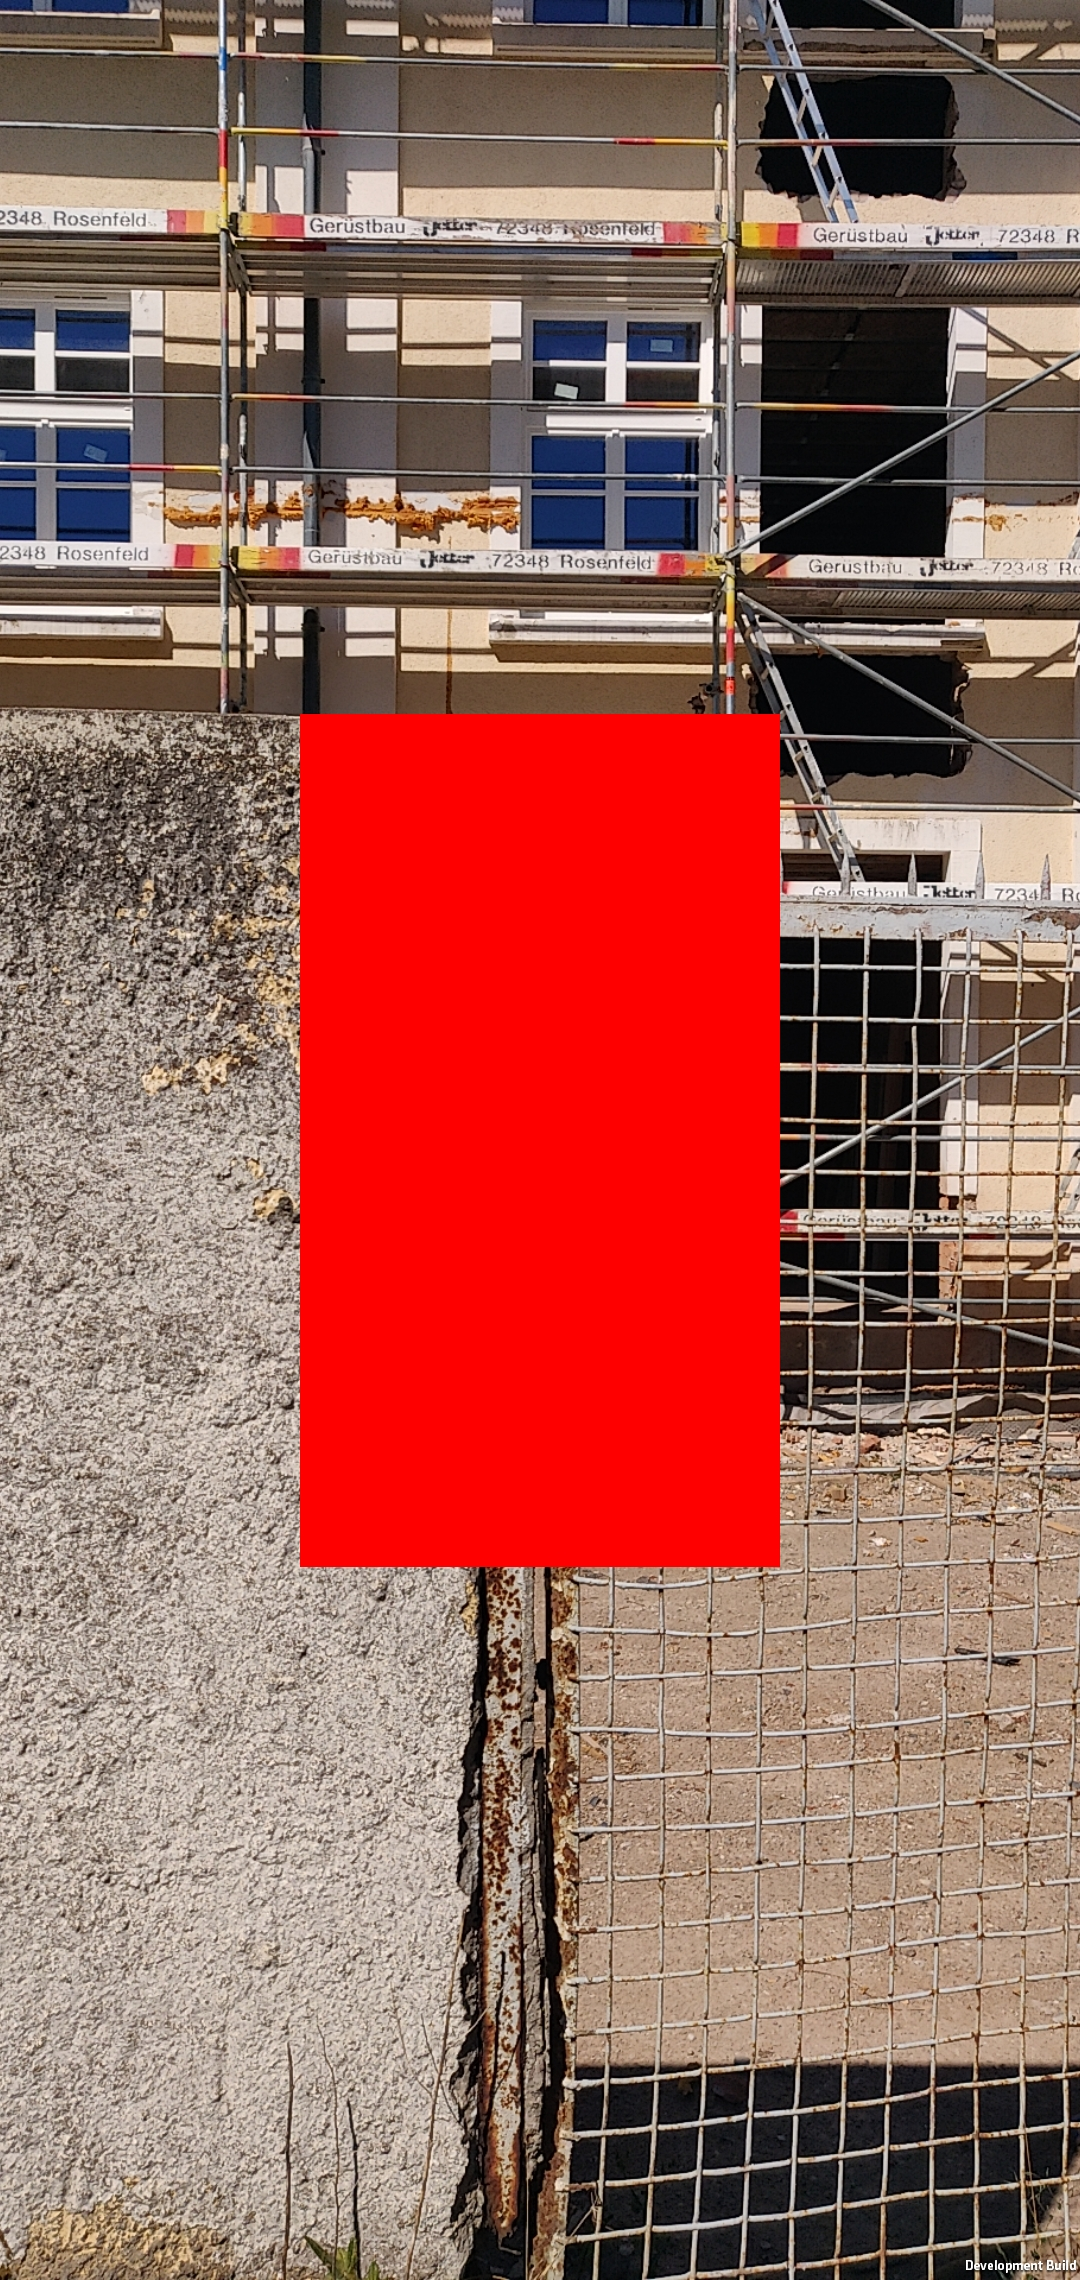
\includegraphics[width=0.3\linewidth]{img/anwendung/arcore/arcore-depth-occlusion.jpg}}%
    \qquad
    \subfloat[][]{\includegraphics[width=0.3\linewidth]{img/anwendung/arcore/arcore-depth-occlusion-2.jpg}}%
    \qquad
    \subfloat[][]{\includegraphics[width=0.3\linewidth]{img/anwendung/arcore/arcore-depth-occlusion-3.jpg}}%
    \qquad
    \caption{Die Depth Map aus einer Entfernung von 1,5m (a) im Vergleich zu der Depth Map aus 1m (b) und die Szene selbst mit der Mauer und dem Zaun aus 1,5m Entfernung(c).}%
    \label{fig:technische-umsetzung-arcore-depth-problem}
\end{figure}
% Ungenauigkeiten, auch auf andere Paper hinweisen
% GPS Experiment
% Vergleich Google Koordinaten und Vermessungsamt Koordinaten
In der Regel sind bei der Nutzung von GPS Positionsabweichungen von bis zu 10 Metern möglich. Eine genaue Platzierung der Gebäude ist daher problematisch.
% Abbildung mit Beispiel

Um die Tracking-Genauigkeit zu erhöhen, gibt es mehrere Methoden. \textit{DGPS (engl. Differential GPS)} verbessert GPS-Signale, indem es ein Korrektursignal durch eine ortsfeste Referenzstation mit bekannter Lokalisierung berechnet. Da es in Deutschland lediglich acht solcher Stationen gibt und einige Anbieter nur kommerziell die Daten bereitstellen, ist diese Methode nicht für diese Arbeit geeignet\footnote{https://www.heise.de/newsticker/meldung/Differential-GPS-und-WLAN-RTT-Praezise-Ortung-mit-Android-P-4046935.html} \footnote{Liste von DGPS-Sendern: https://www.ndblist.info/datamodes/worldDGPSdatabase.pdf}. Eine weitere bekannte Möglichkeit bietet \textit{SBAS (engl. Satellite Based Augmentation System)}, bei dem mehrere geostationäre Satelliten das GPS Signal auf bis zu einem Meter Genauigkeit zu verbessern \cite*{doerner}.

Platinsky et al.\cite{platinsky} erstellen für ein besseres Tracking bei fehlender GPS Genauigkeit ein 3D-Modell der Umgebung. Bei der anschließenden AR Nutzung in diesem Gebiet wird auf dem Smartphone SLAM betrieben. Die Daten vom Smartphone werden mit der 3D-Karte verglichen, um ein genaueres Tracking durchzuführen.
% GPS Genauigkeit
% - Experiment GPS
% -- GPS Daten vom Vermessungsamt im Vergleich zu Google
% Kompass Genauigkeit
% - Jiggle mit Filter weg
% Mobile Limitierungen
% - Anzahl Polygone der vorhandenen Gebäude
% - Shader -> kein Raytracing
% - Occlusion ohne Tiefensensor


%KAPITEL 6 Future Work
% Sonne nochmal anpassen
% Occlusion mit ARKit testen
% Tiefenkamera verwenden, um Nebel/Dunst zu simulieren
% Blitzeinschläge simulieren
% Partikeleffekte für Schnee (Schnee liegt auf Dach)
% Label mit dem Namen und Infos zum Gebäude in AR
% Benutzung der App als grundlage für andere Projekte
% - Eigene Gebäude reinladen und mit entsprechenden Daten darstellen
% Neumodellierung der Gebäude -> weniger Polygone -> mehr einzelne Materialien, die angepasst werden können

%KAPITEL Fazit

% ANHANG
% UML Klassen Auflistung

\newpage\pagestyle{empty}\null\newpage\pagestyle{plain}
\raggedright
%\printbibliography[heading=bibintoc,title={\bibname}] % \bibname is the default name, you can customize it
\newpage
\addcontentsline{toc}{section}{\listfigurename} % \listfigurename is the default name, you can customize it
\listoffigures       % Example figures
\newpage\pagestyle{empty}\null\newpage\pagestyle{plain}
\raggedright
%\printbibliography[heading=bibintoc,title={\bibname}] % \bibname is the default name, you can customize it
\newpage
\addcontentsline{toc}{section}{\listfigurename} % \listfigurename is the default name, you can customize it
\listoffigures     % List of figures, bibliography
\addcontentsline{toc}{section}{Eidesstattliche Erklärung}
\thispagestyle{plain}

{\parindent0pt

    \Large
    \textbf{Eidesstattliche Erklärung}

    \vspace{1cm}

    \normalsize
    Ich erkläre hiermit an Eides statt, dass ich die vorliegende Thesis selbständig und ohne
    unzulässige fremde Hilfe angefertigt habe. Alle verwendeten Quellen und Hilfsmittel sind
    angegeben.

    \vspace{1cm} \par
    \docCity, \docDeadline \par
    \vspace{1cm}
    \line(1,0){200} \par
    \docAuthor

} % Eidesstattliche Erklärung 
\printbibliography
\end{document}